\documentclass[../thesis.tex]{subfiles}

% graphics path
\graphicspath{
  {../../figures/methods/},
  {./../figures/methods/}
}

\begin{document}
\chapter{Numerical Modeling of Vapor Intrusion}

\import{./}{abstract.tex}

% TODO: Restructure to reflect the COMSOL workflow
% - Keep main body simple
% - Use appendices as building/lego blocks to add complexity, e.g. one appendix about how to model a PP, and just that.

% TODO: Move model section as its own chapter.


\import{./}{intro.tex}
\import{./}{geometry.tex}
\import{./}{physics.tex}
\import{./}{indoor.tex}
\import{./}{soil_moisture.tex}
\import{./}{darcys_law.tex}
\import{./}{soil_transport.tex}
\import{./}{meshing.tex}
\import{./}{solvers.tex}
\import{./}{post_processing.tex}
\import{./}{appendix.tex}

\begin{comment}
\section{Introduction}

To formulate a mathematical description of VI, we consider a simple hypothetical VI scenario at steady-state and develop a three-dimensional model of this.
Consider a VI impacted house with a \SI{10}{\metre} by \SI{10}{\metre} foundation footprint with a basement whose foundation lies \SI{1}{\metre} below ground surface (bgs).
There is also a \SI{1}{\centi\metre} wide crack along the perimeter of the \SI{15}{\centi\metre} thick foundation slab, where all contaminant vapor entry into the house is assumed to occur.
Here we will consider the basement alone as the control volume for which the indoor contaminant concentration will be determined.
It is assumed to have a ceiling height of \SI{3}{\metre}, giving a total volume of \SI{300}{\metre\cubed}
and that contaminant vapors are expelled via air exchange with the exterior of the house; the air exchange rate with outdoor air is assumed to be \SI{0.5}{\per\hour}.\par

The contaminant source be the underlying groundwater, which is assumed to be \SI{4}{\metre} bgs, and it is infinitely and homogenously contaminated with TCE (we will normalize everything to this source concentration, so the value does not matter), i.e. the groundwater contaminant concentration does not change over time nor does it have any concentration gradients.
We will only consider contaminant transport in the portion of soil between the open ground surface and the groundwater interface - the \textit{vadose zone}.
This soil is assumed to be homogenous and consist only of \textit{sandy loam} type soil, i.e. there no soil layers, rocks, etc.
For now, we will assume that no contaminant sorption into/onto the soil occurs, but this phenomena will be explored in Chapter (TBD).% TODO: Sorption chapter reference
The house is assumed to be surrounded by open ground that extend \SI{10}{\metre} from the house wall.
Contaminant concentration in the atmosphere is assumed so low that is effectively zero, i.e. contaminant vapors that reach the ground surface are immediately infinitely diluted. \par

The house interior is assumed to be slightly depressurized relative to ambient due to the stack effect; the indoor/outdoor pressure difference is \SI{-5}{\pascal}
This induces an airflow from the ground surface, through the soil, and into the house via the foundation crack.
The airflow interacts with contaminant diffusion in the soil.
Figure \ref{fig:vi_scenario} shows a figure summarizing this VI scenario.\par

% TODO Add a basement to the picture
\begin{figure}
  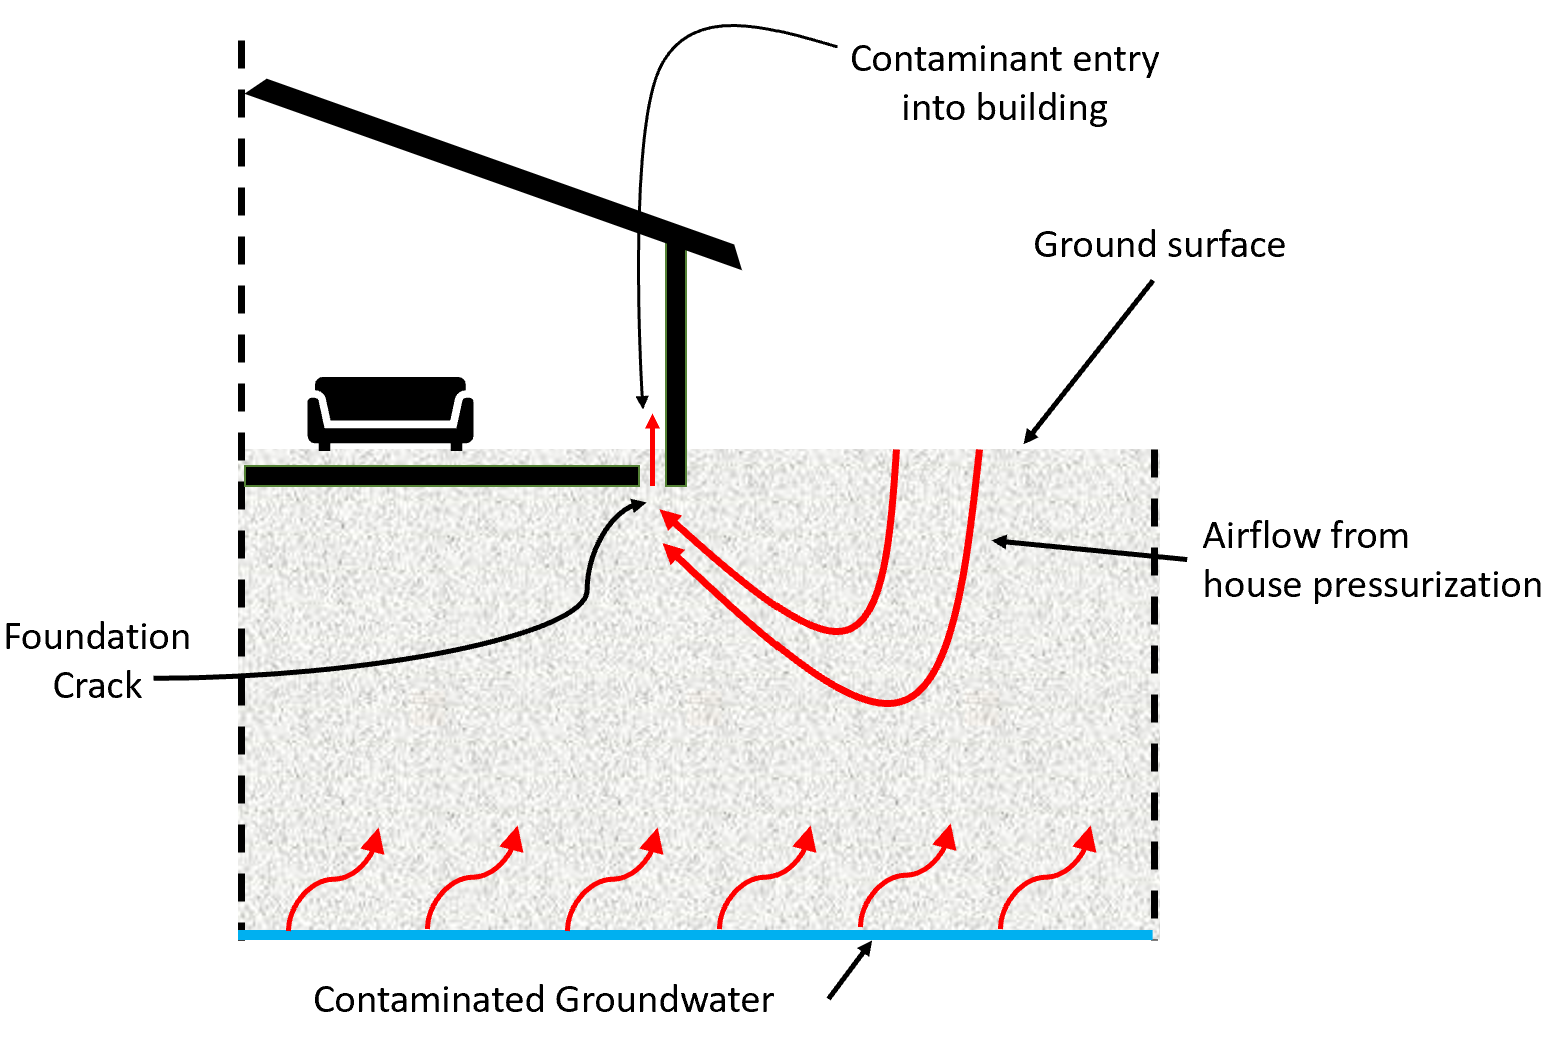
\includegraphics[width=\textwidth]{model_cartoon.png}
  \caption{The considered VI scenario.}
  \label{fig:vi_scenario}
\end{figure}

The basement interior will be modeled as a continuously stirred tank reactor (CSTR), (but without reactions), where the indoor contaminant concentration will depend on the contaminant entry rate $n_\mathrm{ck}$ from the soil via the foundation crack and the air exchange rate $A_e$.
The details of this will be covered section \ref{sec:indoor}.\par

To determine $n_\mathrm{ck}$ the contaminant transport in the soil needs to be modeled.
This will be done using the advection-diffusion equation, which will be modified for transport in soils.
The contaminant transport itself is driven by a concentration gradient and airflow in the soil.
The contaminant source (groundwater) and sink (atmosphere and contaminant entry into the building) will largely determine the concentration gradient, while the airflow needs to be calculated separately.\par

The airflow in the soil is modeled by Darcy's Law, and is driven by a pressure gradient in the soil, which induced by the indoor/outdoor pressure difference.
Details are in section \ref{sec:darcys_law}.\par

One last consideration is that the vadose zone is partially saturated with water, with the soil pores more or less filled near the groundwater interface, and with soil moisture content decreasing as a function of elevation above groundwater $z$ [\si{\metre}].
The soil moisture content has a profound effect on transport in the soil; it restricts both the airflow and contaminant diffusivity in the soil.
Thus, the soil moisture content $\theta_w$ must first be determined in order to solve the contaminant transport and Darcy's Law.\par

The resulting physical system is highly coupled, with many physical aspects dependant on others.
Figure \ref{fig:physics_overview} shows the coupling between each physicsal process, its output, and how it relates to the other processes that ultimately determine VI.\par

% TODO Add Millington-Quirk blob
\begin{figure}
  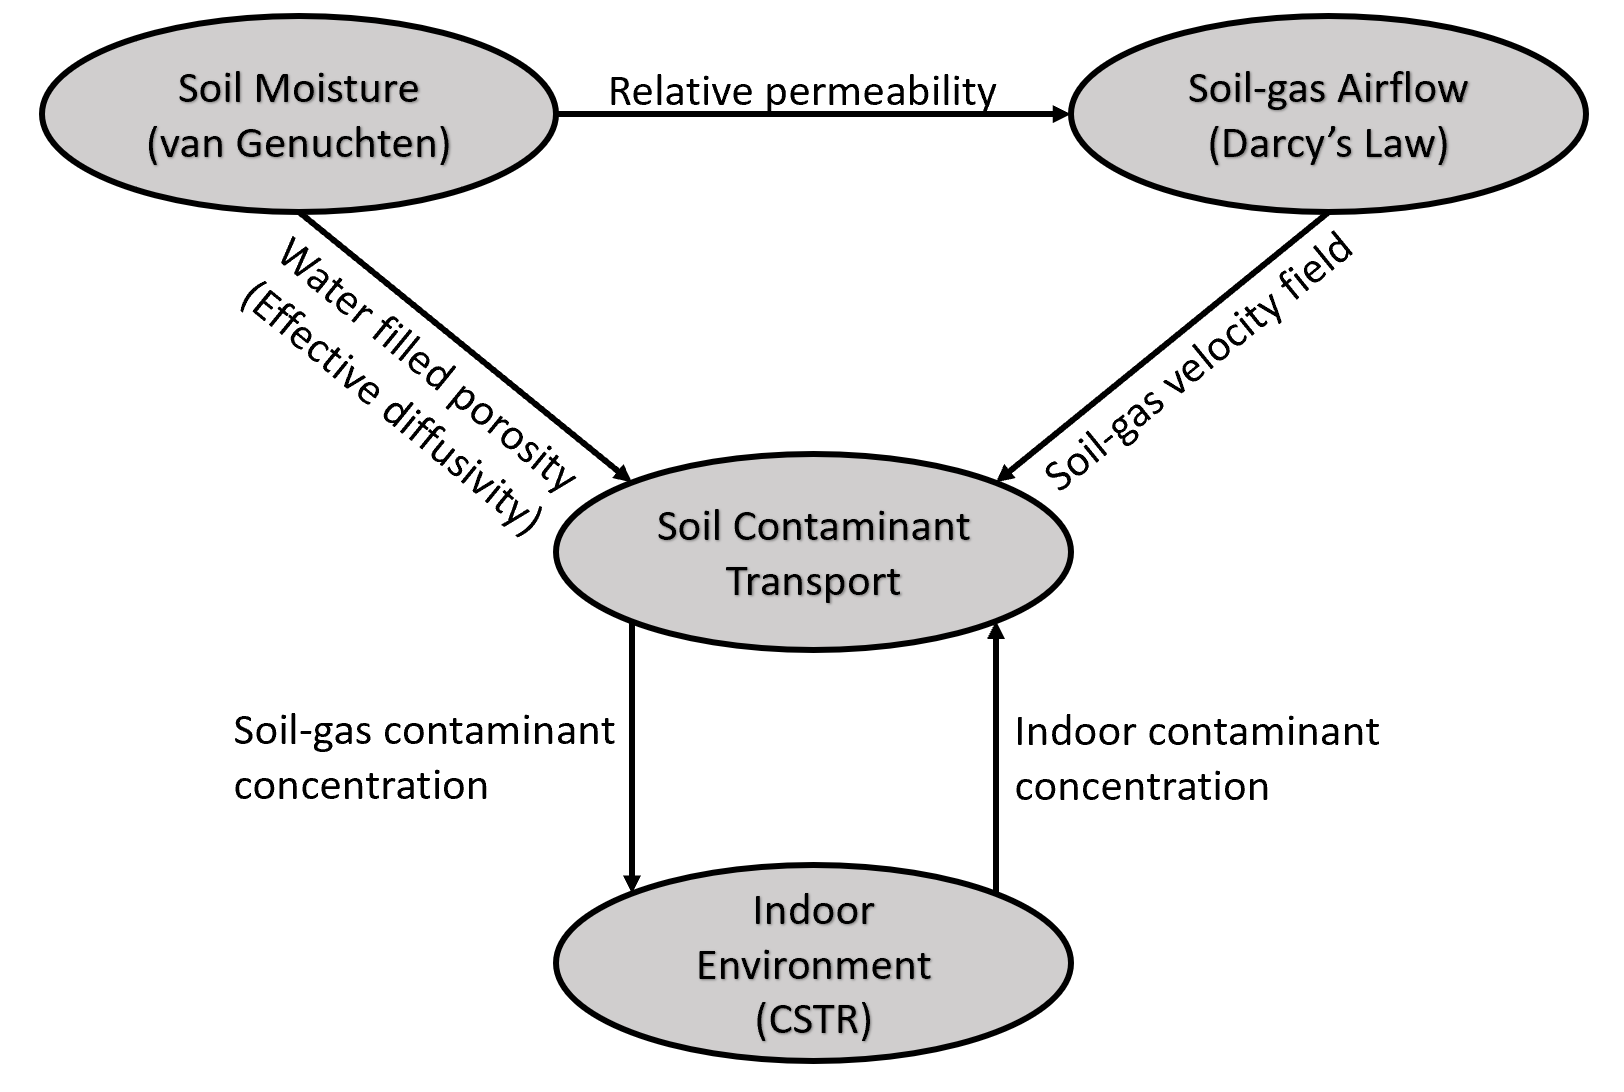
\includegraphics[width=\textwidth]{physics_interaction.png}
  \caption{Coupling between the physics used to model VI.}
  \label{fig:physics_overview}
\end{figure}

In this chapter, we will walk through the process of numerically modeling this VI scenario using the finite element method (FEM) and post-processing of the results.
A discussion regarding past and present VI models, their advantages and limitations, will follow.\par

\subsection{Finite Element Method}

% TODO Make it clear which sources I use here and say so early.
% TODO Make a figure showing the basis functions with nodal coefficients.

Many physical phenomena are described by partial differential equations (PDEs), but for anything but the simplest scenarios, these do not have an analytical closed-form solutions; therefore numerical methods are needed for finding an approximate solution.
This is achieved by discretizing the problem, i.e. transforming a continuous problem into a discrete one.
There are numerous ways to discretize a problem, and some of the more popular schemes are finite difference (FDM), finite volume (FVM), and finite element method (FEM).\par

In this work we use FEM, which is a popular numerical scheme that offers some distinct advantages over other schemes for modeling VI.
FEM subdivides the domain of the PDE problem into many smaller subdomains called elements.
These elements can take a wide variety of shapes, e.g. tetrahedra, prisms, or cuboids for three-dimensional problems and triangles or rectangles for two-dimensional problems.
The collection of elements that make up the domain or geometry is called a \textit{mesh}.
The fineness of the mesh is what largely determines the accuracy of the solution, but also increases the computational costs.\par

The size of each element can be highly nonuniform which allows FEM to discretize complicated geometries.
This is advantageous for modeling VI, where different parts of the geometry can have dramatically different resolution requirements; the \SI{1}{\centi\metre} foundation crack requires elements on the scale of \si{\milli\metre}, while in other parts of the geometry the resolution requirement is on the scale of \si{\metre}.
This ability to easily represent complicated geometries with elements of ununiform sizes helps maintain accuracy while saving computational resources.
Another benefit of using these elements is that it is easy to assign different constant values throughout the domain, and heterogenous materials can easily be represented.\par

The purpose of this work is not to provide a detailed description of the FEM, but for the interested reader \citeauthor{larson_finite_2010}\cite{larson_finite_2010} is a good resource.
However, it is important to know that FEM assumes that the approximated solution to a PDE can be written as a series of linear functions, called \textit{basis functions}.
\begin{equation}
  u \approx u_h = \sum^i u_i \psi_i
\end{equation}
here $u$ is the exact solution to the problem;
$u_h$ is the approximate solution;
$u_i$ is a \textit{nodal coefficient};
and $\psi$ is a \textit{basis function}.
These basis functions are usually some simple function, e.g. a hat function or some lower-order polynomial.\par

These basis functions are used to discretize the problem by rewriting a PDE into its \textit{weak form}, multiplying the equation with another set of functions called a \textit{test function}.
The test functions are the same type of function as the basis function, i.e. if the basis function is a hat function, so is the test function.
The result of this is an integral, where the integrands are the product of the basis function.
These integrals are numerically solved using some quadrature method, which gives a linear system of equations.
This system of equations is then solved to give all of the $u_i$ coefficients and thus the approximated solution $u_h$.\par

The point of this is that choice of basis function, i.e. hat function, first or third order polynomial, can influence the accuracy of the solution, and certain basis functions are more appropriate for certain PDEs.
Generally, higher order polynomials will give a more accurate solution, but at a computational cost, making it sometimes difficult to choose.
This adds another level of complexity of using FEM over some other numerical schemes, as the accuracy of the solution is not only influenced by the mesh but also somewhat by the choice of basis functions.
This highlights one of the drawbacks of FEM, i.e. that it is mathematically more challenging to implement and use than some other numerical schemes may be.\par

Fortunately, due to the attractiveness of the method, many commercial FEM packages have developed which increases usability significantly.
In this work we will use such a package - COMSOL Multiphysics, where subsequent sections will cover the steps required to implement our VI model in COMSOL.
(Of course, this could easily be translated into use in another software package.)\par

In order, we will cover:
\begin{enumerate}
  \item Creation of a model geometry.
  \item Defining physics/governing equations, boundary, and initial conditions.
  \item Discretize/mesh the geometry.
  \item Solver configuration.
  \item Post-process the results.
\end{enumerate}

\section{Geometry Generation}

Designing a good model geometry is critical as it can save significant computational resources.
When designing a geometry the FEM user should try to represent the model geometry as accurately as possible while:
\begin{enumerate}
  \item Avoid unnecessarily fine details; these may require an excessively fine mesh to resolve.
  \item Leverage symmetry to reduce the domain size over which solution must be effected, and thereby the mesh can be made finer in a smaller portion of the domain.
\end{enumerate}\par
Achieving these goals is not always straightforward, and success depends on the skill of the modeler and on the available tools.
Typically a model geometry is constructed in some computer assisted design (CAD) software, and the particular tools available in these packages vary.
While not absolutely necessary, the usa of a CAD package outside of the COMSOL solver might sometimes make development of the domain description easier.\par

\begin{figure}[htb!]
  \centering
  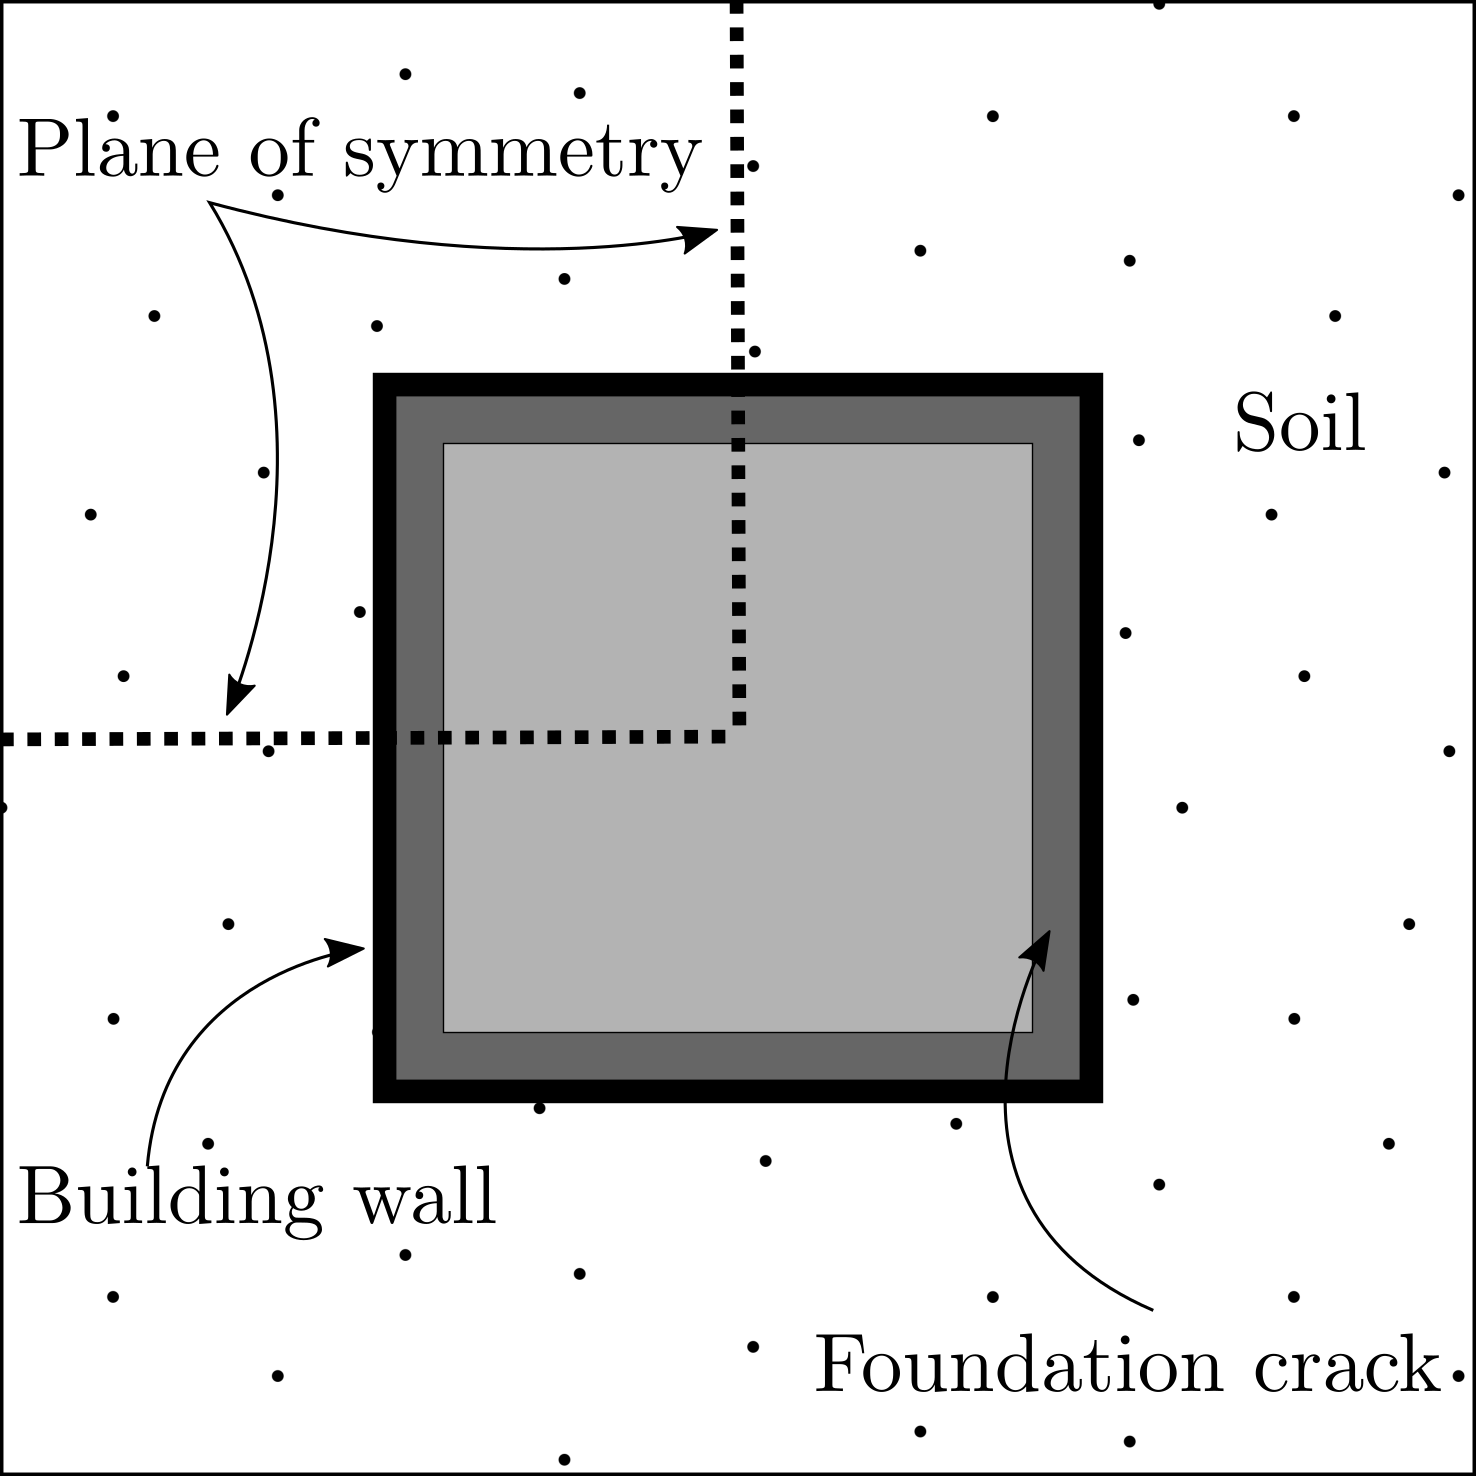
\includegraphics[width=0.75\textwidth]{symmetry.png}
  \caption{Birds-eye view of the VI scenario, showing the foundation and the breach, building wall, as well as the plane of symmetry that allows only a quarter of the total domain to be generated.}
  \label{fig:symmetry}
\end{figure}

COMSOL has a built-in geometry generation tool, which allows the construction of advanced geometries by performing various operations on simpler geometries, e.g. a cylinder and half sphere can be combined to make a rivet.
But as noted, it is also possible to import pre-generated geometries from other CAD software.
For present illustrative purposes, we will create our own geometry.\par

The interior of the house itself will not be explicitly modeled, instead we only consider the soil surrounding the house.
This is done for the simple reason that it is not important to model the interior of the house.
Once the contaminant is in the structure, the damage, so to speak, has been done.
We are interested in how fast the contaminant enters from the soil, which is what determines indoor contaminant concentration.
In addition, typical building interiors are simply too heterogenous to generalize in any meaningful way.
Trying to explicitly model the interior so as to offer insights into indoor concentration variations while at the same time modeling the necessary subsurface transport, would be prohibitively expensive.
Instead the interior is implicitly modeled as a CSTR and simply coupled with the explicit soil and foundation geometry via the foundation crack boundary.\par

One of the nice properties of the described VI scenario is that, due to symmetry, we only need to explicitly model a quarter of it (see Figure \ref{fig:symmetry}).
This reduces the number of required mesh points by 75\%, which is a huge computational saving.
To create the specified geometry, see the instructions for geometry generation in the appendix.

\begin{figure}[htb!]
  \centering
  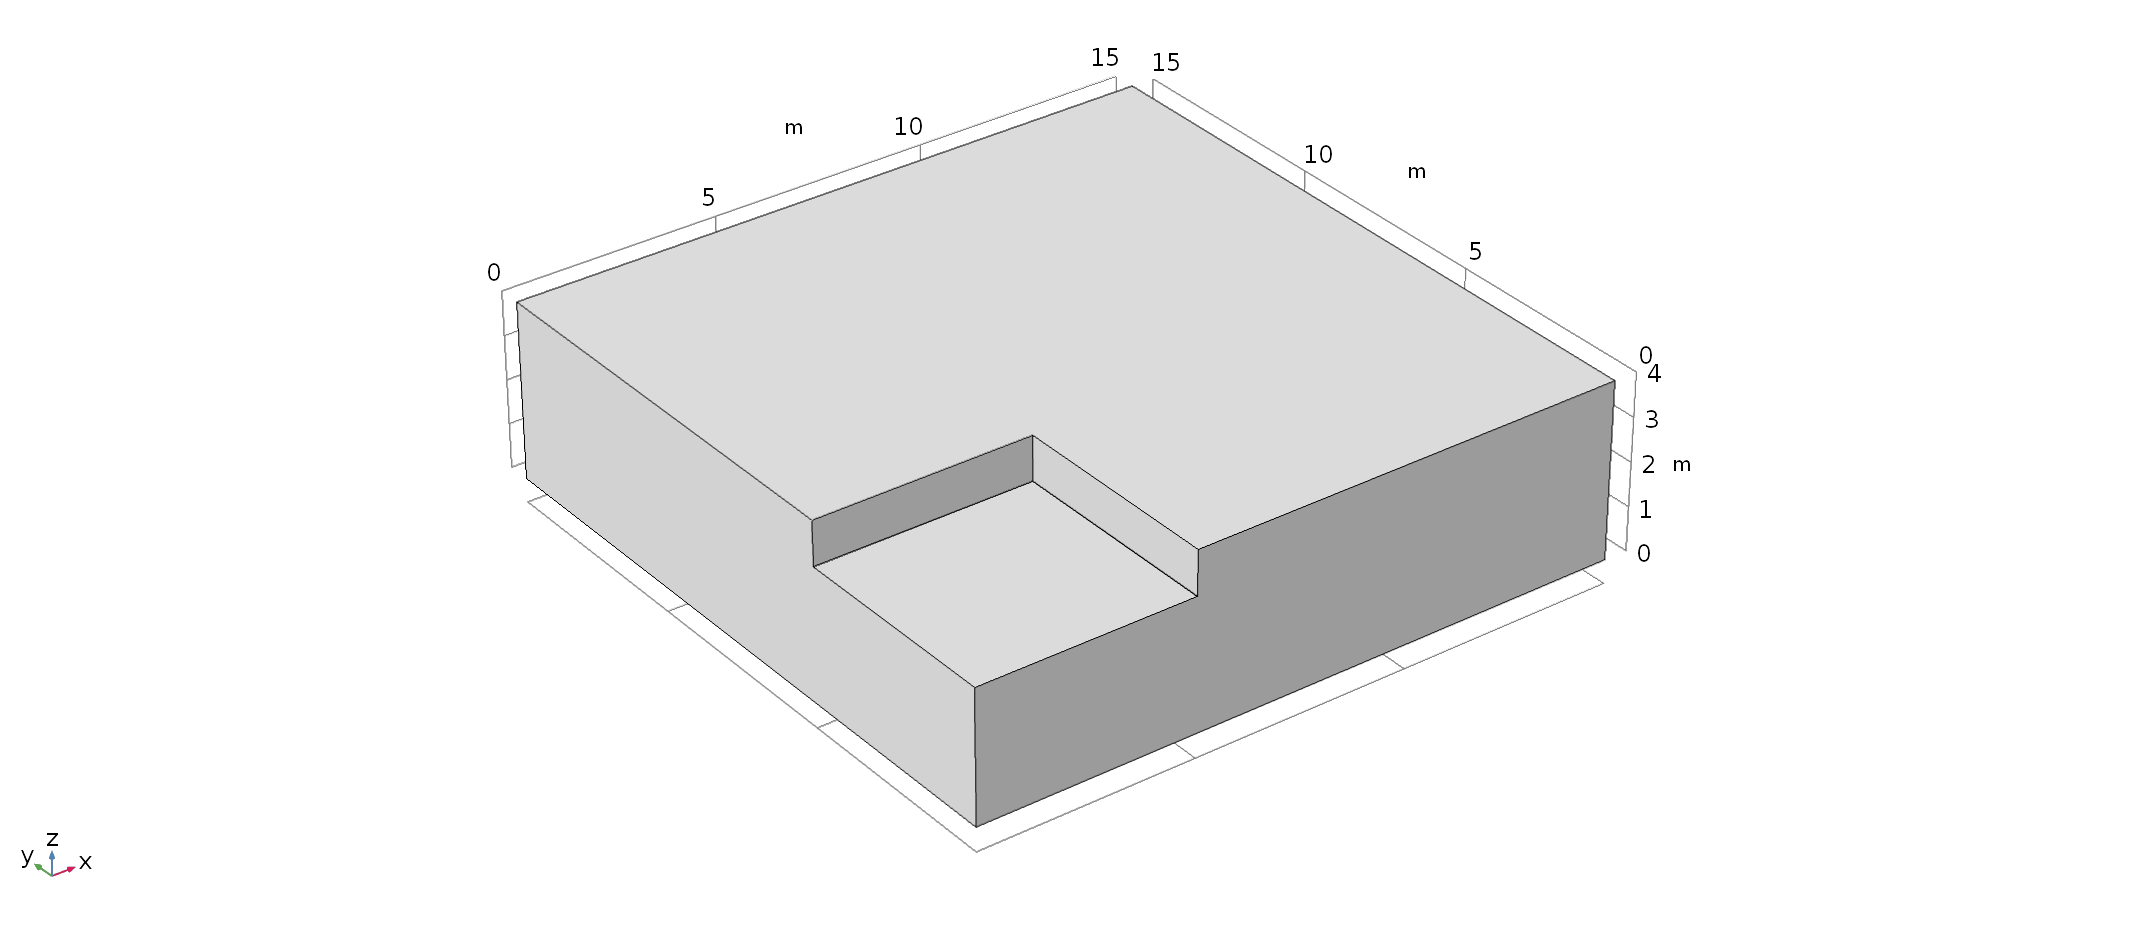
\includegraphics[width=\textwidth]{vi_model.png}
  \caption[VI model geometry in COMSOL]{The complete geometry of the VI scenario as implemented in COMSOL.}
  \label{fig:geometry}
\end{figure}

\section{Vapor Intrusion Physics \& Govering Equations}

% A fantastic introduction/overview

% TODO: Add the figure that shows the relationships between the physics and all of the variables.

\subsection{The Indoor Environment}\label{sec:indoor}

The impacts on the indoor air space is perhaps the most important part of modeling VI, as the goal of these models ultimately is to predict indoor exposure given some external factors.
The indoor environment is, however, only modeled implicitly as a continuously stirred tank reactor (CSTR).
We assume that all contaminant entry into the house occurs via a foundation crack.
It has been shown in other modeling work that results are not overly sensitive to the nature and position of the actual foundation breach\cite{yao_simulating_2013}, so we do not need to be overly concerned about the nature of the crack - the key feature is the overall area that it presents for contaminant entry.
Once the contaminant enters the interior, it is instantly perfectly mixed, which is a key assumption of a CSTR.
Contaminant expulsion occurs via air exchange with the outdoor environment, and is regulated by \textit{air exchange rate} $A_e$, which dictates what fraction of the indoor air is exchanged with outdoor air over a given period of time.
For instance, a common air exchange rate for a house is $A_e = \SI{0.5}{\per\hour}$, i.e. half of the indoor air is exchanged every hour.
The impacts of air exchange rate will be explored in Chapter \ref{chp:preferential_pathways}.\par

It should be noted that in this simple VI model implementation, we assume that there are no indoor sources nor that any sorption of contaminant to/from any indoor materials occurs.
Thus, the reaction term that would ordinarily be part of a CSTR is dropped (but is reintroduced in Chapter \ref{chp:sorption}) and the temporal change in indoor contaminant concentration is thus given by \eqref{eq:cstr}.
\begin{equation}\label{eq:cstr}
  V_\mathrm{bldg}\frac{\partial c_\mathrm{in}}{\partial t} = n_\mathrm{ck} - V_\mathrm{bldg} A_e c_\mathrm{in}
\end{equation}
Here $c_\mathrm{in}$ [\si{\mol\per\metre\cubed}] is the indoor air contaminant concentration;
$n_\mathrm{ck}$ [\si{\mol\per\second}] is the contaminant entry (or exit) rate into the building via the foundation crack;
$A_e = \SI{0.5}{\per\hour}$ is the air exchange rate;
Finally, $V_\mathrm{bldg} = \SI{300}{\metre\cubed}$ is the volume of the house interior (or basement in this case).\par

A limitation of this approach is that we only consider one control volume or compartment, while in reality indoor contaminant concentrations can vary significantly between compartments, in particular between different floors.
There are VI models that use multiple compartments, which in essence are just coupled CSTRs\cite{murphy_multi-compartment_2011}.
Basements typically have higher indoor contaminant concentrations than other floors, so in this implementation we assume that our sole compartment is the house basement, which $V_\mathrm{bldg} = \SI{300}{\metre\cubed}$ reflects.\par

Solving \eqref{eq:cstr} requires us to determine the contaminant entry and air exchange rates.
Air exchange rates can vary quite significantly, and are a significant source of temporal variability in VI, a topic that will be further explored in Chapter \ref{chp:preferential_pathways}.
However, they typically vary around relatively well-known values as air exchange rates are regulated in building codes.
For residential buildings, it is typical that air exchange rate is around $A_e = \SI{0.5}{\per\hour}$ and thus for simplicity we will choose this value.\par

\paragraph{Contaminant entry into the building}

Contaminant entry rates are significantly more difficult to determine, as they depend on air velocity through the foundation breach and the concentration gradient across it.
The determination of these is the main point, and challenge in VI modeling.\par

\begin{figure}[htb!]
  \centering
  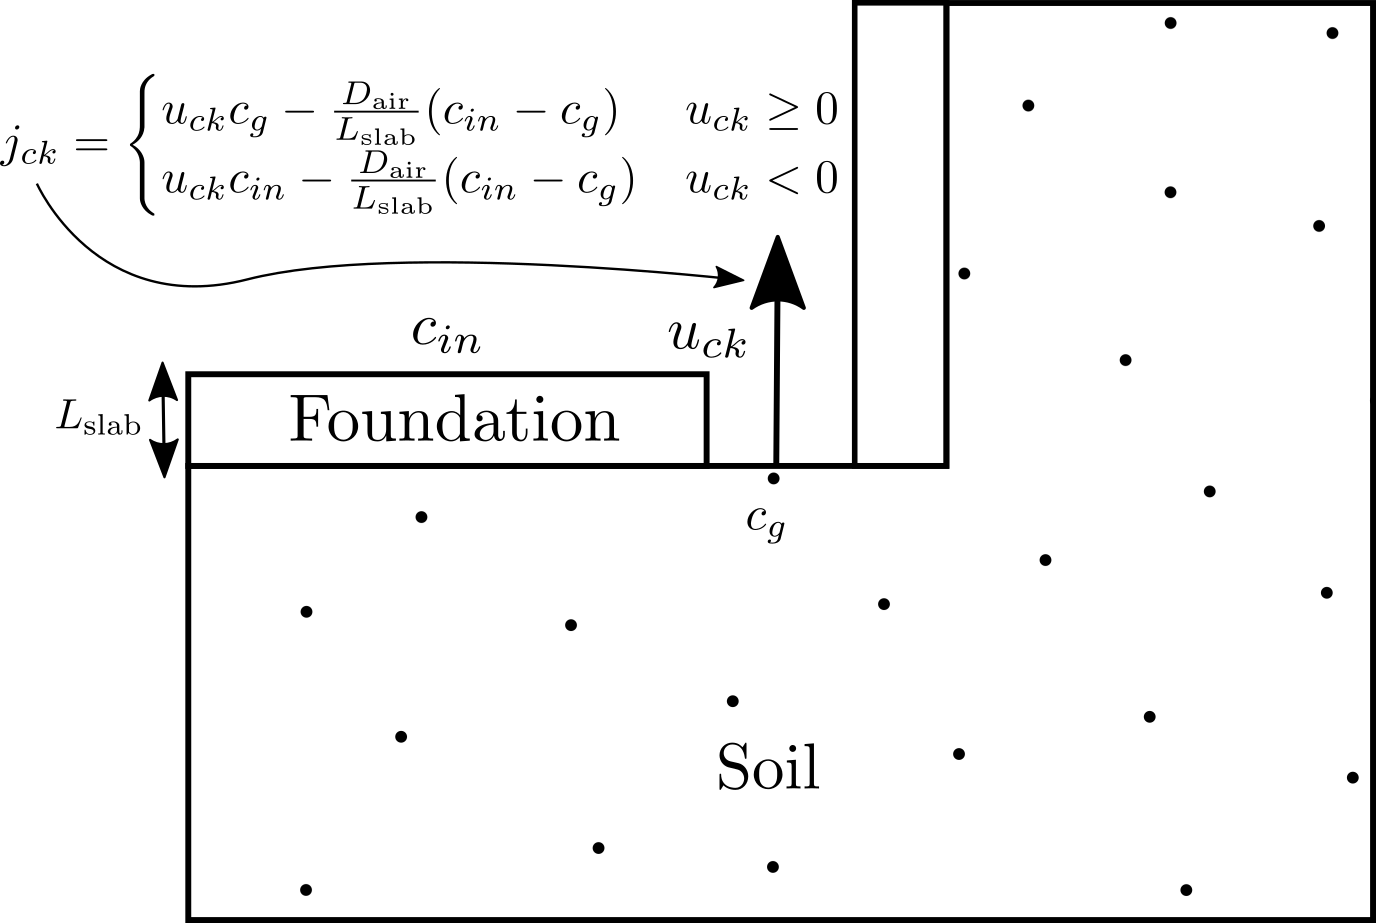
\includegraphics[width=0.6\textwidth]{crack_transport.png}
  \caption[Schematic of soil-gas contaminant entry into a building through a breach in the foundation.]{Soil-gas contaminant vapors are transported from the underlying soil into a building via a breach in the foundation. The scale is exaggerated, and in our modeled scenario the crack is only \SI{1}{\centi\metre} wide.}
  \label{fig:crack_transport}
\end{figure}

The contaminant entry $n_\mathrm{ck}$ is given by integrating the contaminant entry flux $j_\mathrm{ck}$ across the foundation crack boundary $A_\mathrm{ck}$.
\begin{equation}
  n_\mathrm{ck} = \int_{A_\mathrm{ck}} j_\mathrm{ck} dA
\end{equation}
The contaminant flux through the foundation crack is modeled as transport between two parallel plates and has an advective and a diffusive component.
\begin{equation}
  j_\mathrm{ck} = j_\mathrm{advection} + j_\mathrm{diffusion}
\end{equation}
Since contaminant concentration indoors is lower than it is in the soil or near foundation crack region a concentration gradient from the soil-gas to the indoor will exist.
The interior of the crack is not explicitly modeled, but assumed to only contain air and thus we assume the diffusion coefficient is the same as in air.
\begin{equation}
  j_\mathrm{diffusion} = - \frac{D_\mathrm{air}}{L_\mathrm{slab}} (c_{in} - c_g)
\end{equation}
here $D_\mathrm{air} = \SI{7.2e-6}{\metre\squared\per\second}$ is the diffusion coefficient of TCE in air as a sample contaminant of interest; other contaminant of common concern have comparable diffusivities.
$L_\mathrm{slab} = \SI{15}{\centi\metre}$ is a typical thickness of a foundation slab;
$c_{in}$ [\si{\mol\per\metre\cubed}] is the indoor contaminant concentration;
$c_g$ [\si{\mol\per\metre\cubed}] is the contaminant gas-phase concentration at the foundation crack boundary.\par

Advective transport through the slab can occur in both directions, i.e. contaminants can be carried from the soil into the house and from the house into the soil\cite{holton_creation_2018}.
The direction of this transport depend on the direction of the flow, with a positive sign indicating that airflow goes into the house.
\begin{equation}
  j_{advection} = \begin{cases}
    u_{ck} c_g & u_{ck} \geq 0 \\
    u_{ck} c_{in} & u_{ck} < 0
\end{cases}
\end{equation}
here $u_{ck}$ [\si{\metre\per\second}] is the airflow velocity through the foundation crack.

Thus the total contaminant transport through the foundation crack is given by \eqref{eq:contaminant_entry}.
\begin{equation}\label{eq:contaminant_entry}
  j_{ck} = \begin{cases}
    u_{ck} c_g - \frac{D_\mathrm{air}}{L_\mathrm{slab}} (c_{in} - c_g) & u_{ck} \geq 0 \\
    u_{ck} c_{in} - \frac{D_\mathrm{air}}{L_\mathrm{slab}} (c_{in} - c_g) & u_{ck} < 0
\end{cases}
\end{equation}
(See Figure \ref{fig:crack_transport}.)
Not only will \eqref{eq:contaminant_entry} be used to calculate the contaminant entry rate into house, but it is a necessary boundary condition for calculating the contaminant concentration in the soil.
However, as we see, \eqref{eq:contaminant_entry} is a function of both the soil-gas concentration at the foundation crack boundary $c_g$ and the indoor contaminant concentration $c{in}$, thus these two are coupled and need to be solved simultaneously.\par

\begin{comment}

To cover:

- Description of the physics that cause the variable soil moisture
- Modeling this
  - Correy & Brooks
  - van Genuchten

- Description of van Genuchten


\end{comment}
% TODO: How do I cite here when I basically use the same source for everything?

\subsection{Variable Soil Moisture Content}\label{sec:van_genuchten}

The portion of soil between groundwater and ground surface is variably saturated with water and is called the vadose zone.
Under environmental conditions, TCE and many other contaminants are miscible in water, and will be partitioned between its dissolved and vapor phases, which has profound effects on the total contaminant transport in the vadose zone.
The rates of diffusion in liquids and gases usually differ by orders of magnitudes. % TODO: Source
Likewise, advective transport in the two phases are vastly different, and as such it is important to account for the varying soil moisture content.\par % TODO: Source

Water filling of soil pores from groundwater is driven by a negative pressure gradient induced by surface tension, called capillary potential and is here represented by $\psi$.
This capillary potential is a function of the soil moisture content, and becomes increasingly negative as the water content decreases, and is zero when the soil matrix is saturated with water.
The capillary potential varies with the hydraulic properties of specific soil types.\par

In addition to the capillary potential, soil moisture content is driven by a gravitational potential, e.g. groundwater flow in soil.
The total soil moisture potential $\phi$, is the sum of the capillary and gravitational potentials, here expressed as a pressure head.
\begin{equation}
  \phi = \frac{\psi(\theta_w)}{\rho g} + h_\mathrm{g} = h + h_\mathrm{g}
\end{equation}
where $\phi$ [\si{\metre}] is the total soil moisture potential (as a pressure head);
$\psi$ [\si{\pascal}] is the capillary potential;
$h$ [\si{\metre}] is the capillary potential as a pressure head above the groundwater/soil interface;
$\theta_w$ is the volumetric moisture content by volume soil, i.e. dimensionless;
$\rho$ [\si{\kilo\gram\per\metre\cubed}] is the density of water;
$g$ [\si{\metre\per\second\squared}] is the acceleration due to gravity;
and $h_\mathrm{g}$ [\si{\metre}] is the gravitational potential above a reference plane.\par

In the VI scenario considered here, we assume that there is no gravitational potential, and thus that the soil moisture content is at steady-state.
This simplifies the determination of the soil moisture content, which now is entirely determined by the capillary potential $\psi$, or $h$ in our case.\par

There are two common methods for modeling the capillary potential, one developed by \citeauthor{brooks_properties_1966}\cite{brooks_properties_1966} in 1966, and another by \citeauthor{van_genuchten_closed-form_1980}\cite{van_genuchten_closed-form_1980} in 1980.
Both of these are semi-empirical approaches and relies on experimentally determined parameters for a specific soil type to be used.
In this work, we only use van Genuchten's method, simply because parameters for a wide variety of soils have been made available by the EPA and may be seen in Table \ref{tbl:soils}.\par

If the assumption that there is no gravitational potential cannot be made, then the full soil moisture potential $\phi$ needs to be determined.
This is achieved by solving Richard's equation.\par % TODO: Write about Richard's equation and reference it?

\subsubsection{van Genuchten's Soil-Water Retention Model}

% TODO: Make sure the sign or absolute |h| should be here or not.
The relationship between capillary pressure and moisture content is called \textit{soil moisture retention}, and is what van Genuchten's method models.
Specifically, his method models the water saturation of the soil and is given by \eqref{eq:van_genuchten_saturation}.
\begin{equation}\label{eq:van_genuchten_saturation}
  \mathrm{Se} =
    \begin{cases}
      \frac{1}{(1 + (\alpha |h|)^n)^m} & h < 0 \\
    1 & h \geq 0
    \end{cases}
\end{equation}
here $\mathrm{Se}$ is the saturation, which ranges from 0 to 1, where 1 is fully saturated with water;
$\alpha$, $m$, and $n=\frac{1}{1-m}$ are the empirically determined van Genuchten parameters and can be seen in Table \ref{tbl:soils};
and $h$ [\si{\metre}] is the capillary pressure head, which in this case is the elevation above the groundwater/soil interface.\par

It is important to note that $\mathrm{Se} = 0$ does not mean that there is no moisture in the soil, but soils retain a small amount of water in the matrix - residual moisture content (which again is soil specific).
Thus, the soil moisture content is given by \eqref{eq:van_genuchten_soil_moisture}
\begin{equation}\label{eq:van_genuchten_soil_moisture}
  \theta_w =
    \begin{cases}
      \theta_r + \mathrm{Se}(\theta_t - \theta_r) & h < 0 \\
      \theta_t & h \geq 0
    \end{cases}
\end{equation}
where $\theta_w$ is the volumetric soil moisture content;
$\theta_t$ is the soil porosity;
and $\theta_r$ is the residual moisture content.\par

By extension, the soil gas or air content is given by
\begin{equation}\label{eq:gas_porosity}
  \theta_g = \theta_t - \theta_w
\end{equation}
An example of the soil saturation and moisture content as a function of pressure head is shown in Figure \ref{fig:retention_curve}.
Note the steep decline in moisture content near the groundwater interface - that is the capillary zone and we will see that it presents a significant barrier to contaminant transport from the groundwater in section \ref{sec:transport}.\par

\begin{figure}
  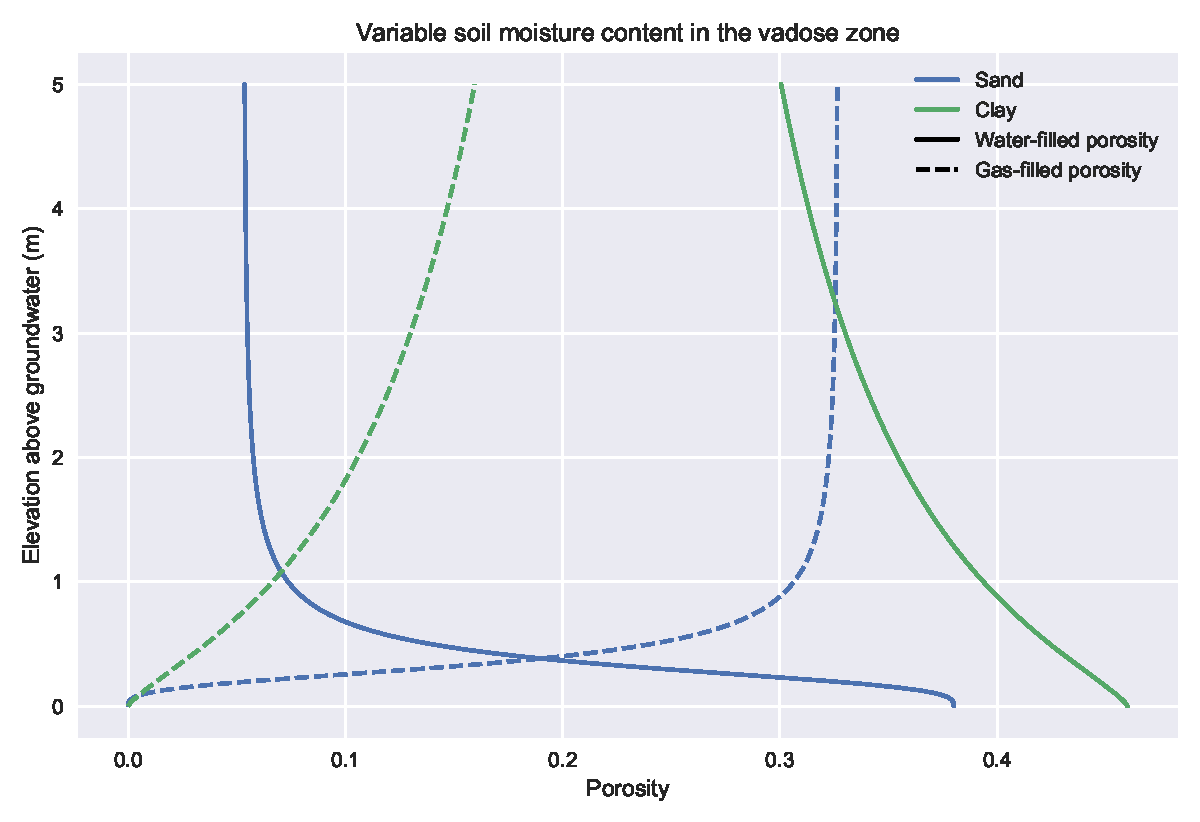
\includegraphics[width=\textwidth]{van_genuchten.pdf}
  \caption{Example of a soil moisture retention curve as a function of pressure head above the groundwater/soil interface.}
  \label{fig:retention_curve}
\end{figure}

The presence of water in the soil matrix has profound implications for transport as the pore space may be restricted to only one phase.
For instance, in the capillary zone, the only possible bulk transport in the water phase, while gas phase transport is impossible.
The opposite is true near the ground surface, where most of the pore space consists of air.\par

Soil already limits transport for a single phase due to its permeability, i.e. it is harder to pump water through a soil columns than a pipe of the same size.
This extra phase-specific transport inhibition is modeled as a \textit{relative permability} and is given by \eqref{eq:van_genuchten_relative_permeability}.
\begin{equation}\label{eq:van_genuchten_relative_permeability}
  k_r =
    \begin{cases}
      \mathrm{Se}^l \big[ 1 - \big( 1 - \mathrm{Se}^\frac{1}{m} \big) \big]^2 & h < 0 \\
      0 & h \geq 0
    \end{cases}
\end{equation}
here $k_r$ is the relative permeability for water; % TODO: Make sure that is right
and $l = 0.5$ is another van Genuchten parameter.\par % TODO: How do I motivate this?

The relative permeability varies from 0 to 1, where 0 indicates that the soil matrix is completely impermeable to the fluid, while a value of 1 means that there is no additional permeability cost.
Since $k_r$ here is relative to water, the gas phase relative permeability is given by $1 - k_r$.
Figure \ref{fig:relative_permeability} shows how the relative gas and water permeability varies in the vadose zone.\par

\begin{figure}
  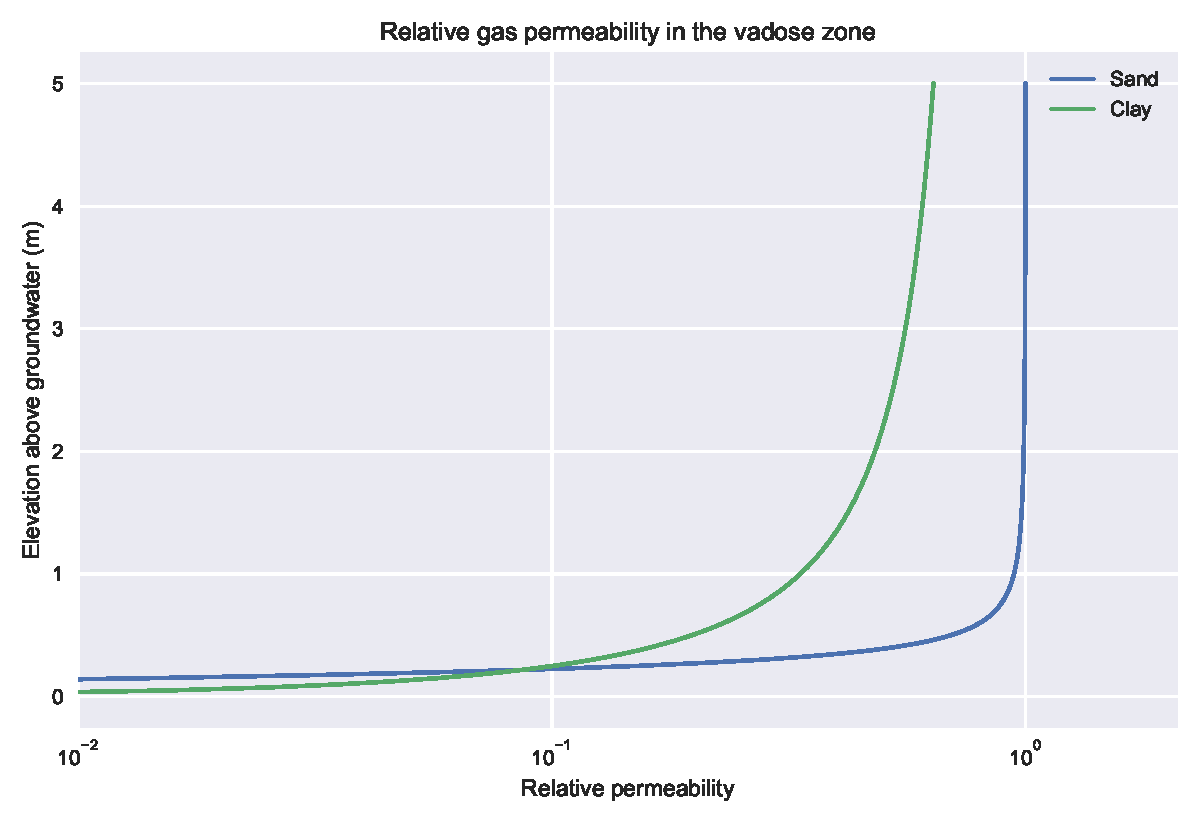
\includegraphics[width=\textwidth]{relative_permeability.pdf}
  \caption{Relative gas and water permeability in the vadose zone or above the groundwater interface.}
  \label{fig:relative_permeability}
\end{figure}

\begin{comment}
% TODO: Move this to where Richard's equation is described.
\begin{equation}\label{eq:van_genuchten_moisture_capacity}
  C_m =
    \begin{cases}
      \frac{\alpha m}{1-m}(\theta_s - \theta_r)\mathrm{Se}^{\frac{1}{m}}\big( 1 - \mathrm{Se}^{\frac{1}{m}} \big)^m & h < 0 \\
    0 & h \geq 0
    \end{cases} \\
\end{equation}
\end{comment}

\subsection{Airflow In The Vadose Zone}\label{sec:darcys_law}

In our VI scenario, the depressurized house induces an advective airflow from the ground surface, through the vadose zone, and into the house via a foundation crack, this flow carries contaminant vapors with it.
This airflow is modeled using a modified version of Darcy's Law.
The modification is made to account for the variable moisture content in the vadose zone, which is discussed in section \ref{sec:van_genuchten}.\par

Darcy's Law describes the flow of a fluid through a porous medium.
This flow is typically driven by a pressure gradient, and its magnitude depends on the permeability of the porous medium and the fluid's viscosity.
\begin{equation}\label{eq:darcys_law_saturated}
  \vec{u} = -\frac{\kappa}{\mu} \nabla p
\end{equation}
here $\vec{u}$ [\si{\m\per\second}] is the airflow velocity vector;
$\kappa$ [\si{\metre\squared}] is the permeability of the porous medium;
$\mu$ [\si{\pascal\second}] is the dynamic viscosity of the fluid;
and $\nabla p$ [\si{\pascal\per\metre}] is the pressure gradient.\par

This \eqref{eq:darcys_law_saturated} formulation of Darcy's Law assumes that the porous medium is saturated with the transporting fluid,\footnote{Darcy's Law also assumes that the flow is in the laminar regime, i.e. the Reynolds number $\mathrm{Re} < 1$.
Due to the small pressure gradients in most VI scenarios, this assumption is rarely unfulfilled, but if it is, then Brinkman's equation should be used instead.}
hence the need to modify this expression when there are two fluid phases present.
While porosity is not directly part of \eqref{eq:darcys_law_saturated}, it is an intrinsic property that determines the permeability $\kappa$ of the porous medium; the degree of saturation in pores determines the air permeability.
This variation in permeability is modeled using the relative permeability expression from van Genuchten's equation \eqref{eq:van_genuchten_relative_permeability}.
The effective soil permeability is the product of the saturated soil permeability and its relative permeability giving our modified Darcy's Law \eqref{eq:darcys_law_unsaturated}.
\begin{equation}\label{eq:darcys_law_unsaturated}
  \vec{u} = -\frac{k_r\kappa}{\mu} \nabla p
\end{equation}
Recall that by definition $k_r$ is the relative permeability of the soil to \textit{air}, and thus $k_r\kappa$ form an effective permeability.\par

To calculate the soil-gas velocity field in the vadose zone, we need a continuity equation, which for fluid flow is \eqref{eq:fluid_continuity}.
\begin{equation}\label{eq:fluid_continuity}
  \frac{\partial \rho}{\partial t} + \nabla \cdot (\rho \vec{u}) = 0
\end{equation}
Inserting our modified Darcy's Law for the velocity gives \eqref{eq:vapor_transport}.
\begin{equation}\label{eq:vapor_transport}
  \frac{\partial}{\partial t} (\rho \theta_g) + \nabla \cdot \rho \Big( -\frac{(1-k_r) \kappa}{\mu} \nabla p \Big) = 0
\end{equation}
where $\theta_g$ is the gas-filled porosity of the soil from \eqref{eq:gas_porosity};
$\rho = \SI{1.225}{\kilogram\per\metre\cubed}$ is the density of air;
and $\mu = \SI{18.5e-6}{\pascal\second}$ is the dynamic viscosity of air.
Contaminant vapor concentrations are typically very low in VI scenarios, and therefore we assume that the contaminant does not affect the transport properties of air.\par

In order to solve \eqref{eq:vapor_transport} we need to define some boundary conditions.
In our VI scenario, air is pulled from the atmosphere through the ground surface and into the building via the foundation crack.
To model this only three boundary conditions are required.
We also need to choose a basis function, and we use the COMSOL recommended "hat" here, which will be used to determine the pressure $p$ throughout the modeled domain.\par

\paragraph{Boundary Conditions}

The first boundary condition defines a pressure gauge, i.e. a reference point for where the pressure is zero, and is where air will be pulled from.
This is applied to the ground surface boundary.
The second is that we apply the indoor/outdoor pressure difference (-5 Pa) to the foundation crack boundary, assuming that the indoor air pressure exists at the crack entrance at the soil interface.
The third type of boundary condition is applied to all remaining boundaries and is a no flow boundary condition, indicating that no flow passes through these boundaries.
This also applies to the symmetry planes present recalling that we are solving over only a quarter domain.
\begin{align}
  &\text{Ground surface} &p = \SI{0}{\pascal} \\
  &\text{Foundation crack} &p = p_\mathrm{in/out} =\SI{-5}{\pascal} \\
  &\text{Remaining} &-\vec{n}\cdot\rho\vec{u} = 0
\end{align}
where $\vec{n}$ is the boundary normal vector.\par

\paragraph{Initial Conditions}

For steady-state problems, initial conditions are not needed.
Transient simulations however, require initial conditions and these are typically assumed to be given by some steady-state solution that exists before a transient disruption.\par

\subsection{Mass Transport In The Vadose Zone}\label{sec:transport}

To begin deriving a governing equation for contaminant transport in our VI scenario, we consider the continuity equation which states that the change of concentration in some volume of space depends on the advective and diffusive fluxes in and out of the system, as well as any generation or consumption inside the system.
\begin{equation}
  \frac{\partial c}{\partial t} + \nabla \cdot(j_\mathrm{adv} + j_\mathrm{diff}) - G = 0
\end{equation}
here $c$ [\si{\mol\per\metre\cubed}] is the concentration of the chemical species;
$t$ [\si{\second}] is time;
$j_\mathrm{adv}$ and $j_\mathrm{diff}$ [\si{\mol\per\second\per\metre\squared}] are the advective and diffusive fluxes respectively;
and $G$ [\si{\mol\per\second}] is the generation or consumption of the chemical species.\par

In our model we will assume that $G = 0$ as the groundwater is the sole contaminant source, i.e. there are no other sources of TCE in the soil, and TCE also does not readily degrade in soils\footnote{
Although, it is possible to introduce certain bacteria to bioremediate TCE in soils, but this typically requires specific conditions, which generally are not naturally met. Under these specific conditions TCE may be biodegraded by some bacteria\cite{fan_biodegradation_1993,little_trichloroethylene_1988}
}.
However, this term should be retained and an appropriate expression developed if one wants to model:
\begin{itemize}
  \item Biodegradation of some compound in the soil.
  \item Radon intrusion (remember radon gas is generated throughout soils and rocks).
  \item A soil or subsurface source, e.g. a leaky tank or evaporation from a liquid contaminant spill.
\end{itemize}\par

The advective flux is given by
\begin{equation}
  j_\mathrm{adv} = \vec{u} c
\end{equation}
where $\vec{u}$ [\si{\metre\per\second}] is a velocity vector.
The diffusive flux is given by Fick's Law
\begin{equation}
  j_\mathrm{diff} = -D \nabla c
\end{equation}
where $D$ [\si{\metre\squared\per\second}] is the diffusion coefficient of the contaminant in the soil air;
and $\nabla c$ [\si{\mol\per\metre\cubed\per\metre}] is a concentration gradient.
Thus we get the advection-diffusion equation which generally governs transport of a chemical species
\begin{equation}\label{eq:adv_diff}
  \frac{\partial c}{\partial t} + \nabla \cdot(\vec{u} c + -D \nabla c) = 0
\end{equation}
However, this simple gas phase transport equation will not accurately represent contaminant transport in the vadose zone if:
\begin{itemize}
  \item Contaminant transport occurs inside a variably saturated porous matrix which significantly affect transport properties.
  \item The contaminant concentration in the vadose zone is distributed between three phases - gas, water, and solid (via sorption).
\end{itemize}\par

The total contaminant concentration in the soil is given by the sum of the gas, water, and solid phase concentrations at any given point in the soil.
\begin{equation}
  c_T = \theta_w c_w + \theta_g c_g + c_s \rho_b
\end{equation}
Here $\theta_g$ and $\theta_w$ are the gas-filled and water-filled porosities respectively;
$c_T$ [\si{\mol\per\metre\cubed}] is the total soil contaminant concentration;
$c_w$ and $c_g$ [\si{\mol\per\metre\cubed}] are the contaminant concentrations in water and gas respectively;
$c_s$ [\si{\mol\per\kilogram}] is the solid phase or sorbed concentration per mass of soil;
and $\rho_b = (1-\theta_t) \rho$ [\si{\kilogram\per\metre\cubed}] is the bulk density of the soil, which can be calculated from the soil porosity $\theta_t$ and solid phase density of the soil $\rho$ [\si{\kilogram\per\metre\cubed}].\par

The attentive reader will now notice that \eqref{eq:adv_diff} depends on three variables instead of one.
However, remember that we're concerned with low contaminant concentrations, we can relate the gas and liquid phase concentrations via Henry's Law \eqref{eq:henrys_law}
\begin{equation}\label{eq:henrys_law}
  c_g = K_H c_w
\end{equation}
where, for example $K_H = 0.402$ is the dimensionless Henry's Law constant for TCE at \SI{20}{\degreeCelsius}\cite{heron_henrys_1998}.
We also assume that there are no temperature gradients throughout the vadose zone.\par

The solid phase concentration can be related to the others via a linear sorption isotherm.
Here either the gas-solid or water-solid sorption interaction can be chosen; the former is used in Chapter \ref{chp:sorption} where we will explore the effects of gas-solid sorption.
\begin{equation}
  c_s = \begin{cases}
    K_p c_w & \text{Water-solid sorption} \\
    K_p c_g = K_p K_H c_w & \text{Gas-solid sorption}
\end{cases}
\end{equation}
here $K_p$ [\si{\metre\cubed\per\kilogram}] is a sorption partitioning coefficient.\par

Another approach is to simply ignore the role of sorption completely, i.e. $K_p = 0$, which has historically been done in VI modeling and is done in the following parts of this example too.
The reason for this is two-fold.
\begin{enumerate}
  \item Relevant soil sorption data have not been readily available.
  \item At steady-state, sorption doesn't affect the solution; the fact that there is TCE sorbed to soil particles does not influence the vapor transport at steady state, since equilibrium is assumed to have been established prior to the steady-state analysis. This has been a common assumptions in most VI modeling studies, which have mostly focused on steady-state.
\end{enumerate}
Regardless, we will continue carrying the sorption $K_p$ term, because this will become relevant in Chapter \ref{chp:sorption} where experimentally derived relevant sorption data are available, and in which the role of this sorption process is considered in the context of transient models.\par

Using Henry's Law and the linear sorption assumptions we can relate the total contaminant concentration at any point in the soil matrix to the water-phase contaminant concentration at that point, from which the air phase and solid phase concentrations may be immediately calculated.
The focus on water concentration is arbitrary, but commonly used.
\begin{equation}
  c_T = (\theta_w + \theta_g K_H + K_H K_p \rho_b) c_w
\end{equation}
The terms in front of $c_w$ are collected as $R = (\theta_w + \theta_g K_H + K_H K_p \rho_b)$.
This term is called the \textit{retardation factor} and reflects the potentially increased contaminant residence time in the matrix due to transferring between the phases.
Again, this only becomes an important factor in transient transport simulations.\par

In the vadose zone, advective transport can occur in both the water and gas phases inside the soil pores.
\begin{equation}
  j_\mathrm{adv} = \vec{u}_{w,pore} c_w \theta_w + \vec{u}_{g,pore} c_g \theta_g
\end{equation}
here $\vec{u}_{w,pore}$ and $\vec{u}_{g,pore}$ [\si{\metre\per\second}] are the water and gas phase \textit{pore} velocities vectors respectively.
However, from mass conservation, we know that the product of the pore velocity and porosity gives the superficial velocity of a fluid in porous media, i.e. the Darcy's Law velocities.
This together with Henry's Law gives
\begin{equation}
  j_\mathrm{adv} = (\vec{u}_w + \vec{u}_g K_H ) c_w
\end{equation}
and here $\vec{u}_w$ and $\vec{u}_g$ [\si{\metre\per\second}] are the Darcy or superficial velocity vectors.\par

In section \ref{sec:van_genuchten} we assumed that soil-water is stationary, i.e. $\vec{u}_w = 0$ giving
\begin{equation}
  j_\mathrm{adv} = \vec{u}_g K_H c_w
\end{equation}
where $\vec{u}_g$ is the solution obtained from solving Darcy's Law in section \ref{sec:darcys_law}.\par

To model a scenario where there is a gravitational water potential resulting in groundwater flow, one would have to solve two-phase Darcy's Law to get both $\vec{u}_g$ and $\vec{u}_w$.
This significantly complicates the mass transport aspect as well, and as such is beyond the scope of this work.
This rarely contributes much to understanding VI and the rates of groundwater movement are typically too slow to be of much consequence.\par

The diffusive transport expression likewise needs to be adjusted for multiphase systems, and the total diffusive flux through the pore matrix is given by
\begin{equation}
  j_\mathrm{diff} = -(D_w \theta_w \tau_w \nabla c_w + D_g \theta_g \tau_g \nabla c_g)
\end{equation}
here $D_w = \SI{1.02e-9}{\metre\squared\per\second}$ and $D_g = \SI{6.87e-6}{\metre\squared\per\second}$ are the contaminant diffusion coefficients of TCE in pure water and air respectively;
and $\tau_w$ and $\tau_g$ are the water and gas tortuosity terms, reflecting the fact that in a granular bed, the flow does not occur in a straight line direction.\par

Due to the irregular shapes of pores, diffusion of a chemical species will inevitably often occur along a tortuous path, which the tortuosity terms attempt to capture.
As tortuosity depends on the structure of the porous matrix, it is difficult to accurately portray, but a popular approach is to use the Millington and Quirks model\cite{millington_permeability_1961}.
\begin{equation}\label{eq:millington-quirk}
  \tau_w = \frac{\theta_w^{\frac{7}{3}}}{\theta_t^2}, \; \tau_g = \frac{\theta_g^{\frac{7}{3}}}{\theta_t^2}
\end{equation}
here $\theta_t$ is the total or saturated porosity of the soil matrix.
Another popular approach is Bruggeman's model.\par

Combining \eqref{eq:millington-quirk} and \eqref{eq:henrys_law} in our diffusion flux expression gives
\begin{equation}
  j_\mathrm{diff} = -\Big(D_w \frac{\theta_w^{\frac{10}{3}}}{\theta_t^2} + D_g \frac{\theta_g^{\frac{10}{3}}}{\theta_t^2} K_H\Big) \nabla c_w
\end{equation}
the terms in front of $\nabla c_w$ can be collected as an effective diffusion coefficient $D_\mathrm{eff}$ [\si{\metre\squared\per\second}], which with our isothermal vadose zone assumption only depends on the soil moisture content.
Thus we get the final diffusive flux expression
\begin{equation}
  j_\mathrm{diff} = - D_\mathrm{eff}\nabla c_w
\end{equation}
Figure \ref{fig:D_eff} shows how the effective diffusivity varies from being close to that of the pure water diffusivity near the capillary zone, and increases to something closer to gas-phase diffusivity as the soil moisture decreases.\par

\begin{figure}[htb!]
  \centering
  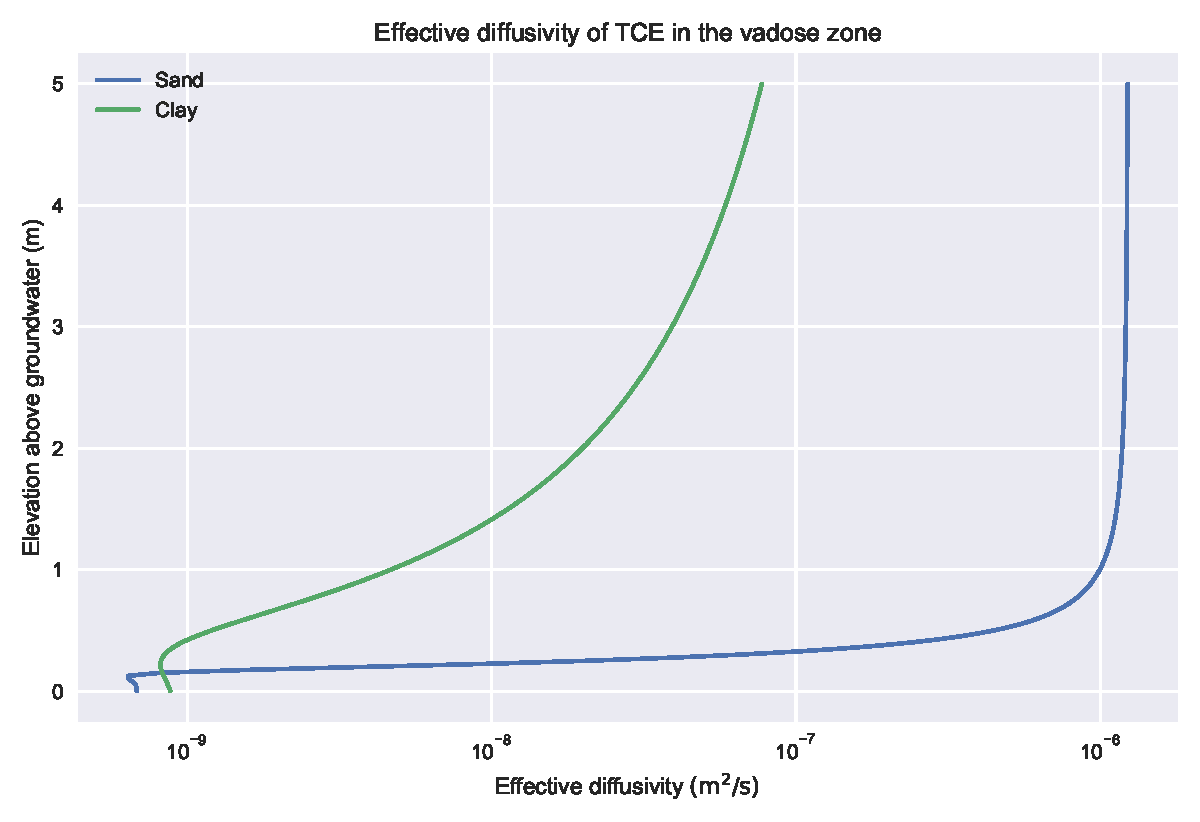
\includegraphics[width=0.75\textwidth]{effective_diffusivity.pdf}
  \caption[Effective diffusivity of TCE in the vadose zone.]{Effective diffusivity of TCE in the vadose zone using the Millington-Quirk model. Soil water and gas filled porosites are calculated using van Genuchten's equations.}
  \label{fig:D_eff}
\end{figure}

Putting all this together finally gives us the governing equation for contaminant transport in the vadose zone for our modeled VI scenario.
\begin{equation}\label{eq:mass_transport}
  R \frac{\partial c_w}{\partial t} = \nabla \cdot (D_\mathrm{eff} \nabla c_w) - K_H \vec{u}_g \cdot \nabla c_w
\end{equation}
To solve this we need to define some boundary and initial conditions.
We also need to choose a basis function which is used to determine the contaminant concentration throughout the domain, and we use the COMSOL recommended second order polynomial here.\par

\paragraph{Boundary Conditions}

In this VI scenario, the sole contaminant source is assumed to be the homogenously contaminated groundwater, which we assume to have a fixed concentration.
The atmosphere acts as a contaminant sink and thus this is simply a zero concentration boundary condition.
Contaminants leave the soil domain and enter the building through a combination of advective and diffusive gas phase transport.
The boundary condition applied to all other boundaries is a no-flow boundary.
\begin{align}
  &\text{Atmosphere} & c_w = \SI{0}{\mol\per\metre\cubed} \\
  &\text{Groundwater} & c_w = c_{gw} = \SI{50}{\micro\mol\per\metre\cubed} \\
  &\text{Foundation crack} & -\vec{n} \cdot \vec{N} = -j_{ck} \; \si{\mol\per\metre\squared\per\second}\\
  &\text{All other} & -\vec{n} \cdot \vec{N} = \SI{0}{\mol\per\metre\squared\per\second}
\end{align}
$\vec{n} \cdot \vec{N}$ is the dot product between the boundary normal vector and the contaminant flux;
$j_ck$ [\si{\mol\per\metre\squared\per\second}] is the contaminant flux into the building from section \ref{sec:indoor}.\par

\paragraph{Initial Conditions}

For steady-state problems, the initial conditions do not enter.
Transient simulations however, require initial conditions and these are assumed to be given by the steady-state solution.\par

\section{Meshing}\label{sec:meshing}

The mesh in FEM model is the collection of small discrete elements that make up the model geometry or domain.
Meshing is the process of generating a mesh.
Meshing is one of the most important aspects of FEM modeling as the mesh directly influences the accuracy of the solution; it is important that the various gradients are resolved by the mesh.
However, designing a good mesh can be challenging as a finer mesh has a higher computational cost.
A good mesh designer must constantly balance accuracy and computational costs by considering where a mesh can be finer and where it can be coarser.\par

The most fundamental unit of the mesh is the element(s) that comprise the mesh.
There are many different types of elements that can be used for meshing and choosing which ones to use depend primarily on the spatial dimensionality of the model, the particularities of the geometry, and the physics that we wish to model.
Obviously different element types are by necessity needed to model a 2D vs. 3D geometry; you cannot mesh a 3D geometry with 2D squares.\par

\begin{figure}[htb!]
  \centering
  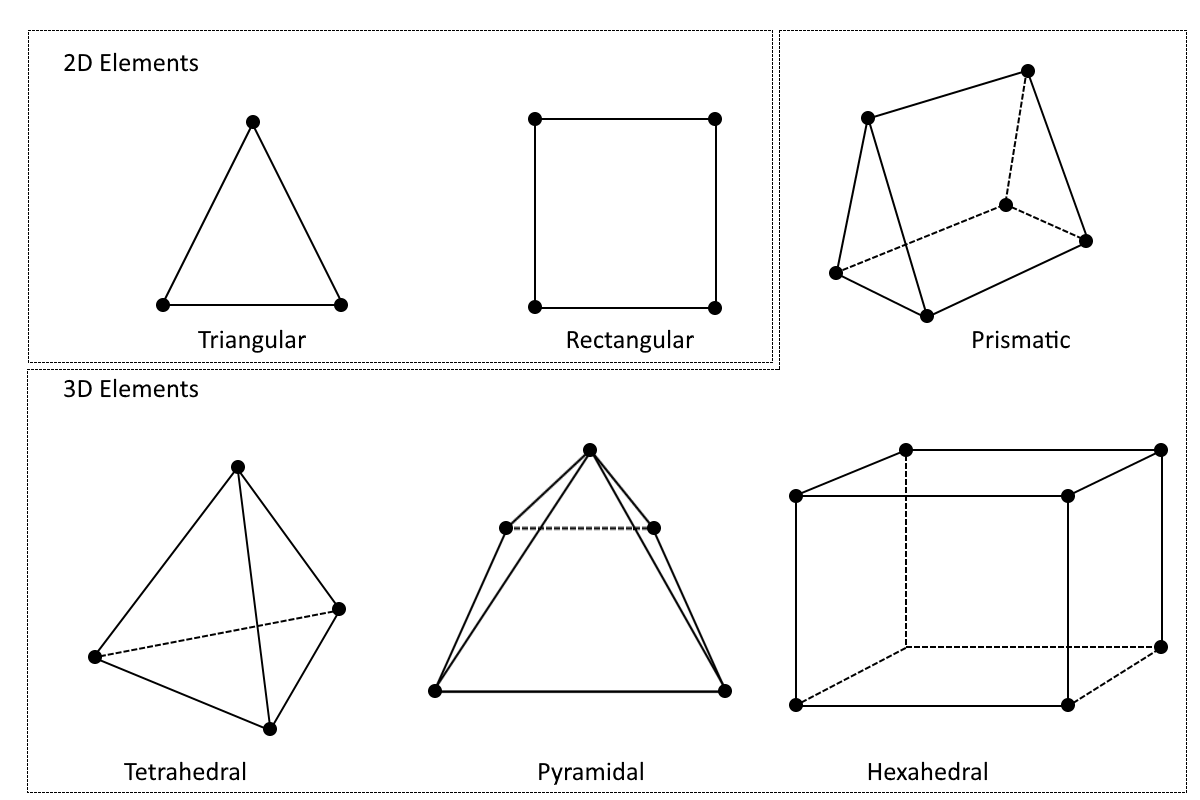
\includegraphics[width=0.75\textwidth]{mesh_elements.png}
  \caption{Some common mesh elements. Figure from COMSOL\cite{noauthor_detailed_nodate}.}
  \label{fig:mesh_elements}
\end{figure}

There are primarily four types of 3D mesh elements available - the tetrahedral, cuboid, prism, and pyramid.
Figure \ref{fig:mesh_elements} shows some common mesh elements.
These can be combined in various ways to represent any 3D geometry.
The most general 3D element is the tetrahedral and will approximate any geometry well.
However, it is not always the most effective choice for meshing a geometry and another element type may be better suited.
This is easiest illustrated with an example.\par

Imagine that you are trying to simulate the laminar flow of some fluid in a pipe.
Because of symmetry, only a wedge of the pipe needs to be explicitly modeled.
Therefore, in this scenario, it might be beneficial to use prism elements rather than tetrahedrals, since these are already wedge shaped.

The laminar pipe flow will have a gradient in the direction of the flow.
Thus the mesh mostly only needs to be fine in the flow direction, while the mesh can be coarser in the radial direction.
Constructing a mesh on this basis would allow us to achieve a solution of high accuracy while still keeping the number of elements relatively small - all through clever mesh design (see Figure \ref{fig:cylinder_mesh}).\par

\begin{figure}[htb!]
  \centering
  \begin{subfigure}{0.49\textwidth}
    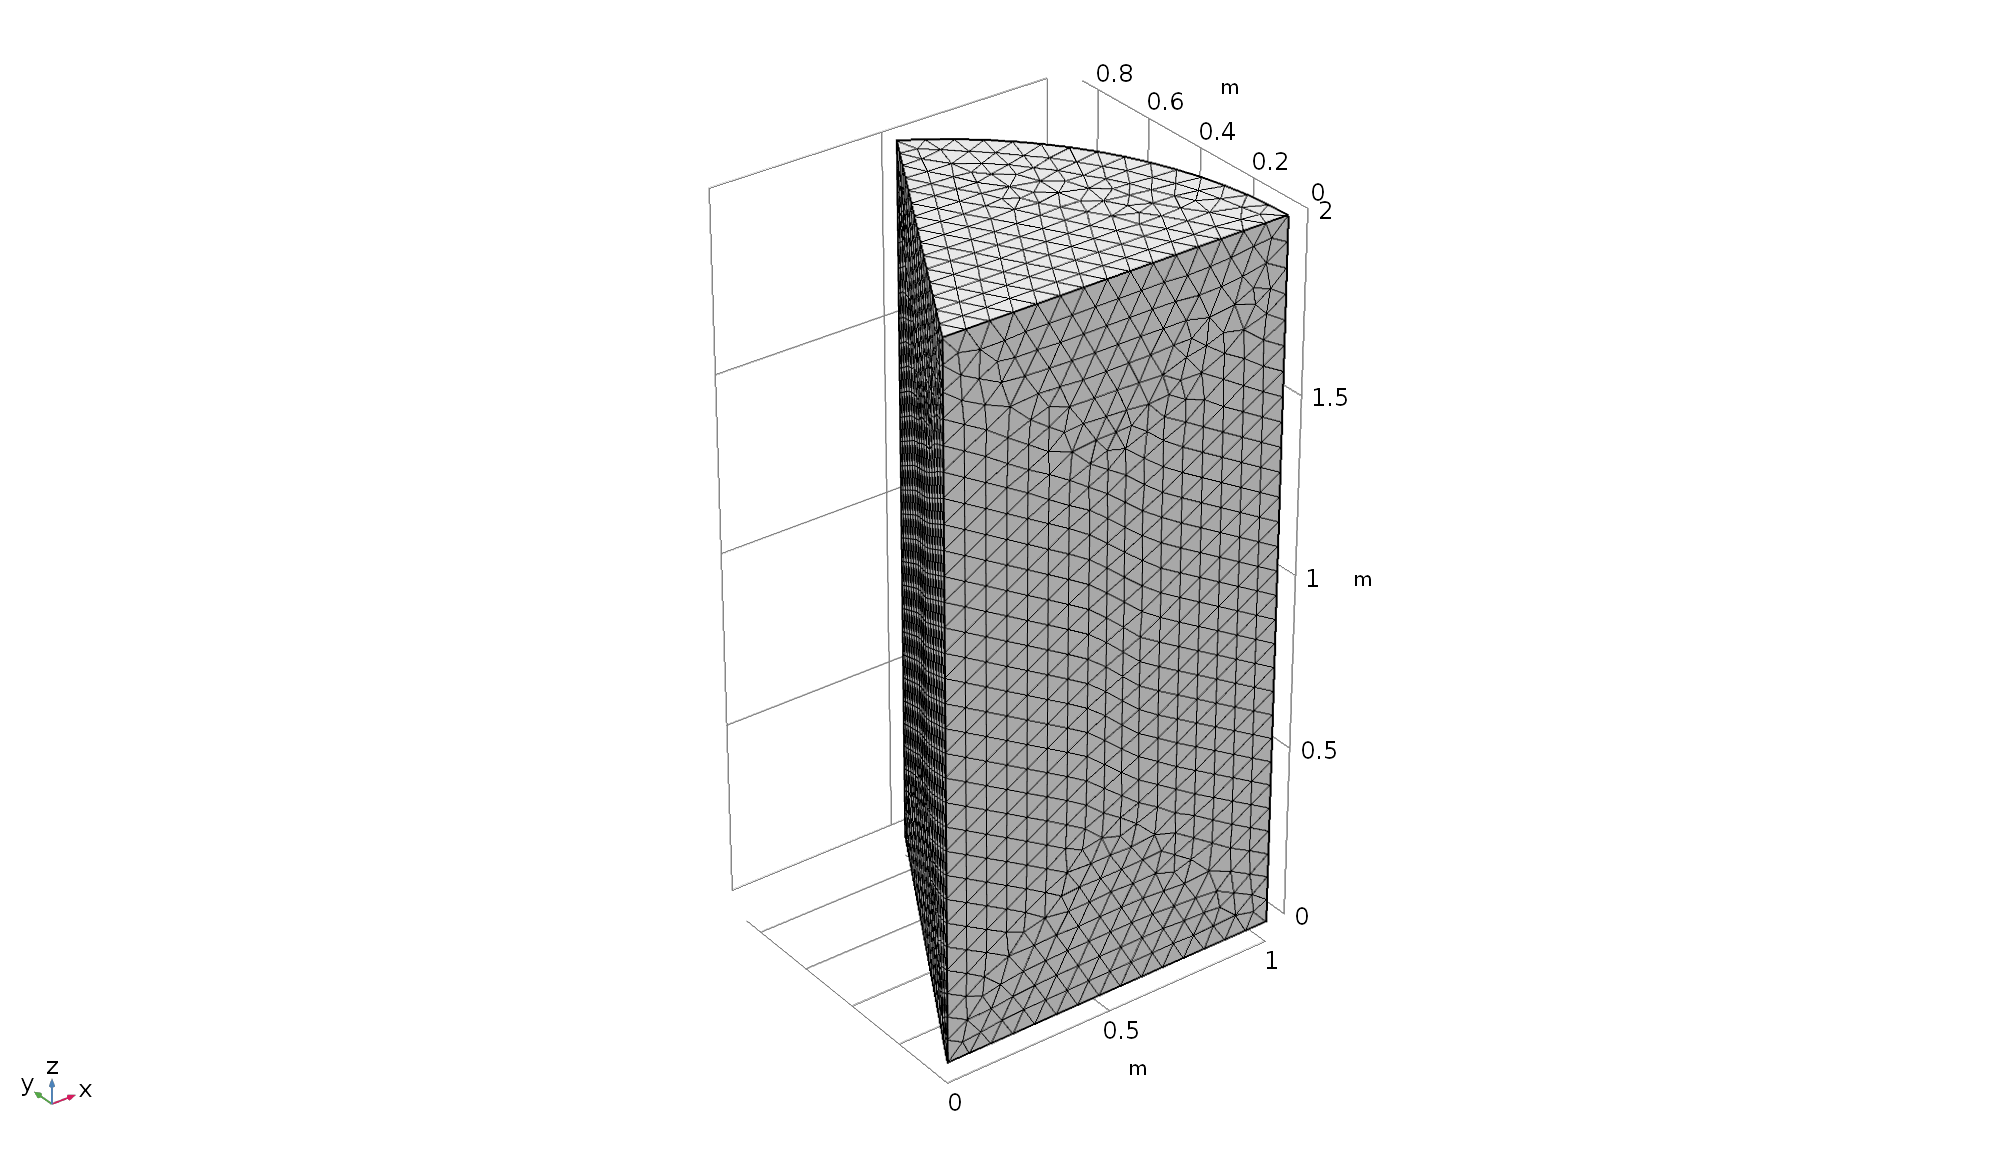
\includegraphics[width=\textwidth]{cylinder_regular_mesh.png}
  \caption{Mesh using tetrahedrals. 50,197 elements.}
  \end{subfigure}
  \begin{subfigure}{0.49\textwidth}
    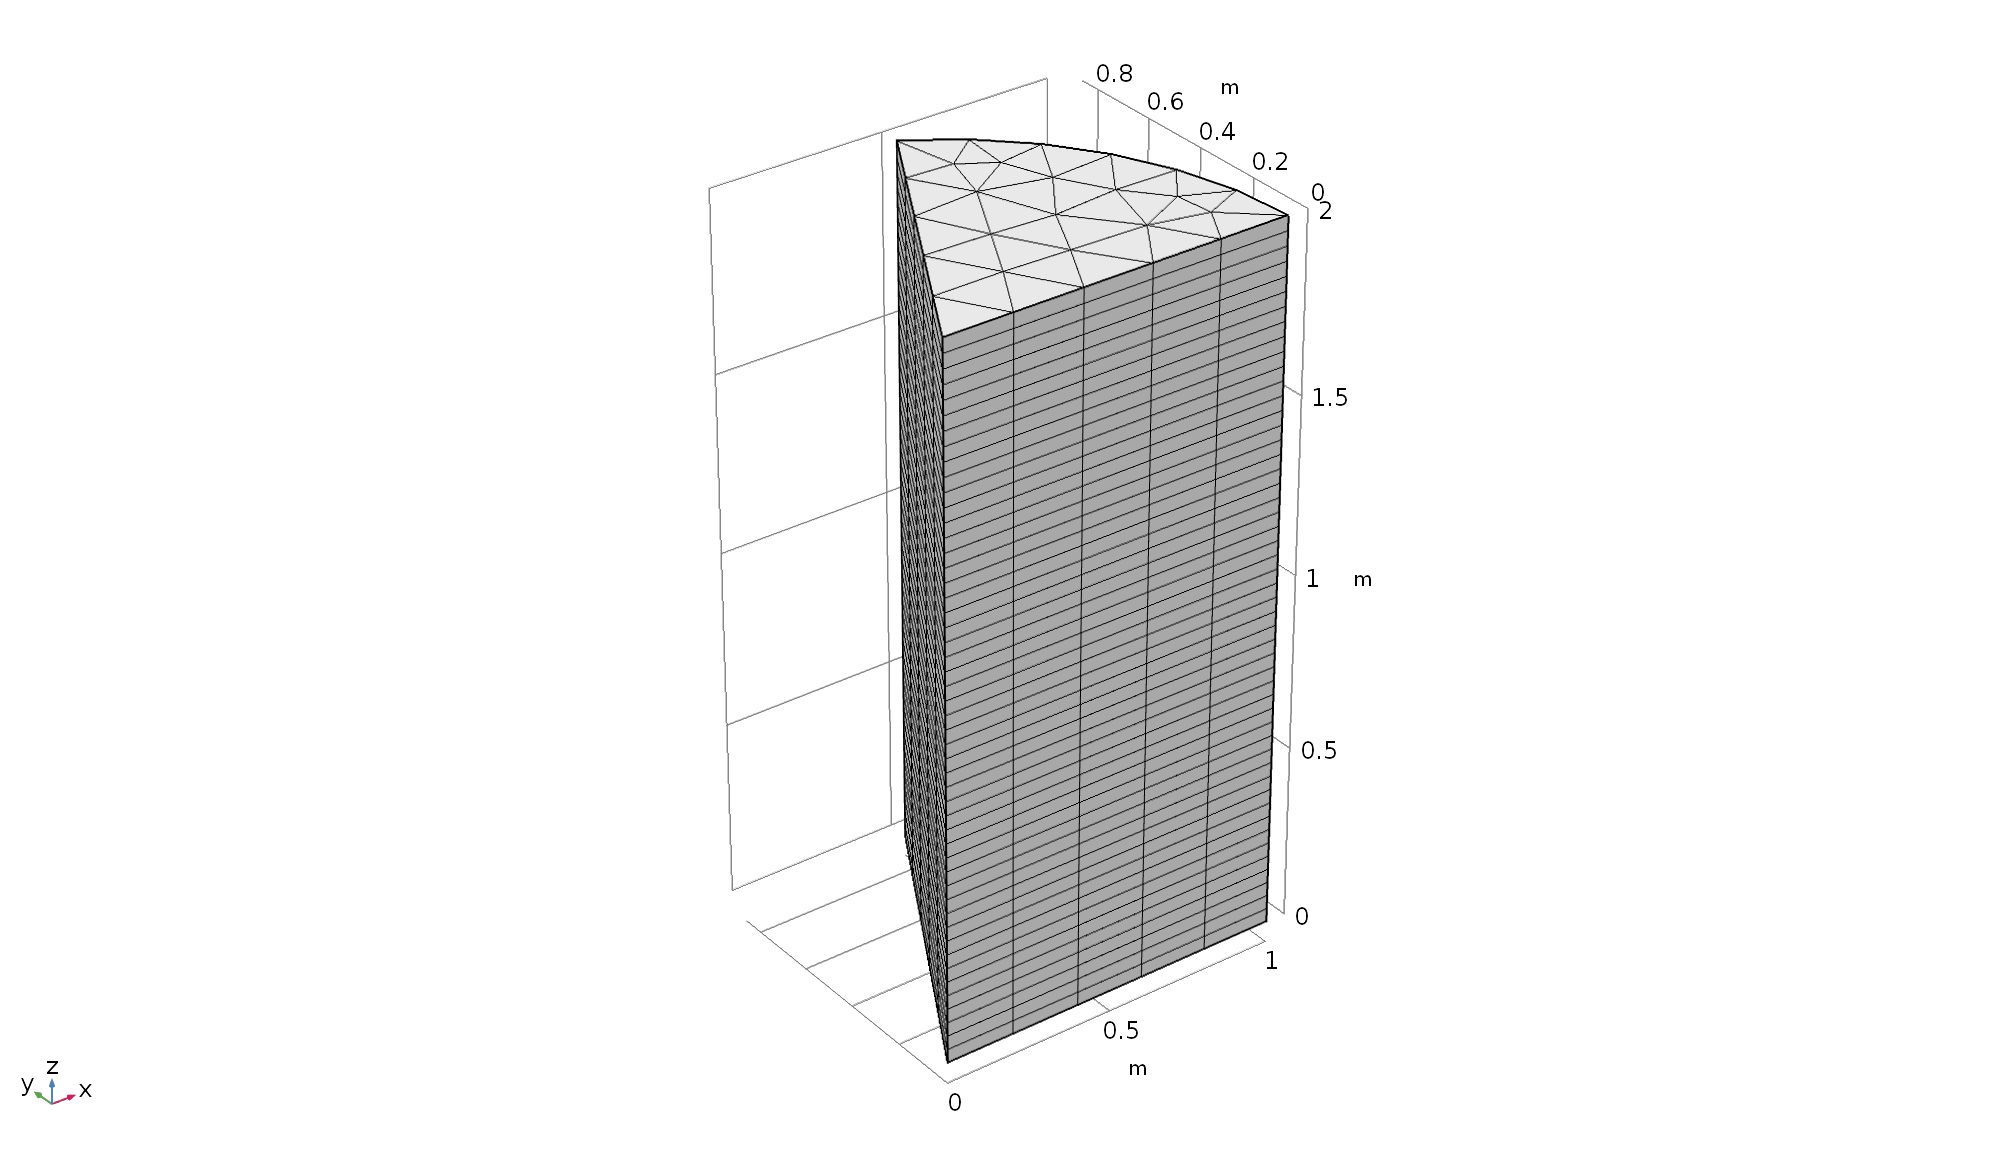
\includegraphics[width=\textwidth]{cylinder_swept_mesh.png}
  \caption{Mesh using prism elements. 1900 elements.}
  \end{subfigure}
  \caption[Example of how physical mesh design can reduce the number of elements.]{By understanding the physics, here considering laminar flow in a pipe (segment), clever mesh design can significantly reduce the number of mesh elements. Notice that the mesh density in the axial direction is more or less the same.}
  \label{fig:cylinder_mesh}
\end{figure}

This is of course a relatively simple example and more complicated geometries may need all kinds of element for constructing a clever design.
These type of multi-element meshes can give significant computational saving but at the expense of often requiring significant user input to be generated.
Sticking to one type of elements is often simpler as these can quickly and easily mesh geometries.\par

Meshing can be done manually, but is often performed by a meshing algorithm.
The creation of these algorithms is a science in itself, but their use often involve passing some basic parameters to the algorithm.
Here the user could, for instance, specify the maximum and minimum element sizes, maximum element growth rate, how finely small features or curves (typically quite difficult to mesh) should be meshed.
These instructions can be specific to various parts of the model, e.g. much finer meshing resolution can be specified for an area of interest and vice versa.
There are also a variety of specialty mesh features such as a mesh boundary layer available: adding finely spaced mesh layers along a boundary.
How to use all of these tools effectively to mesh a geometry is why meshing can be one of the most challenging aspects of FEM modeling.\par

\subsection{Meshing The VI Model}

The first choice we need to make is which type of element to use, and in order to do that we need to think about the gradients of the dependent variables.\par

From van Genuchten's retention curves, we know there will be a large soil moisture gradient in the capillary zone, which will need a relatively fine mesh to be resolved.
The airflow from Darcy's Law will forming some sort of arcing streamline from the ground surface to the foundation crack; the pressure gradient will be inline with these streamline.
The concentration gradient is difficult to predict a priori, but there likely will be some gradient from the groundwater to the ground surface and foundation crack.
Since many of these gradients intersect and go in different directions from each other it makes sense to use tetrahedral elements to mesh the geometry; these are the more general 3D elements.\par

Properly meshing our geometry can be a challenge due to the great range of geometric scale.
The house and soil domains are on the order of meters while the foundation crack is only \SI{1}{\centi\meter} side, and requires very fine meshing.
This is not only due to its small size, but because the contaminant entry will be calculated based on the solution here, which largely determines the indoor contaminant concentration.\par

The COMSOL meshing algorithm only require a few parameters to relatively mesh a geometry with tetrahedrals.
A description of each parameter and its value can be seen in Table \ref{tbl:meshing}.
\begin{table}[htb!]
  \begin{tabularx}{\linewidth}{l c X}
    \toprule
    Input & Value & Description \\
    \midrule
    Maximum element size & \SI{1.5}{\metre} & Maximum size of a element \\
    Minimum element size & \SI{1}{\milli\metre} & Minimum size of a element \\
    Maximum element growth rate & 1.3 & Maximum allowed size increase of adjacent elements. 1.3 indicates that an element can only be 30\% larger than its neighbor. A smaller value gives a finer mesh. \\
    Curvature factor & 0.4 & Ratio between the boundary element size and the geometry curvature radius. A smaller value gives a finer mesh. \\
    Resolution of narrow regions & 1 & Control the number of layers of elements that are created in narrow regions. A larger value gives a finer mesh. \\
    \bottomrule
  \end{tabularx}
  \caption{Inputs to COMSOLs meshing algorithm.}
  \label{tbl:meshing}
\end{table}

\subsection{Boundary Layer Mesh}

When posed with steep gradients in one particular direction at boundaries, as we have here, it is often useful to use a \textit{boundary layer mesh} at the impacted boundaries.
This is a type of mesh that introduces a dense layer of meshes along the normal direction from a boundary.
Boundary layer meshes are common features in meshing algorithms, and COMSOL's is no exception.\par

The number of boundary layers are supplied by the user, and in our case we will use 8 layers, but more could be added if needed.
The distance between each layer is determined by the size of the other elements in its vicinity, as well as the distance growth rate between each layer, which we set to 1.3, i.e. the distance increases by 30\% for each layer.
Figure \ref{fig:mesh} shows our completed mesh.\par

\begin{figure}[htb!]
  \centering
  \begin{subfigure}[b]{\textwidth}
    \centering
    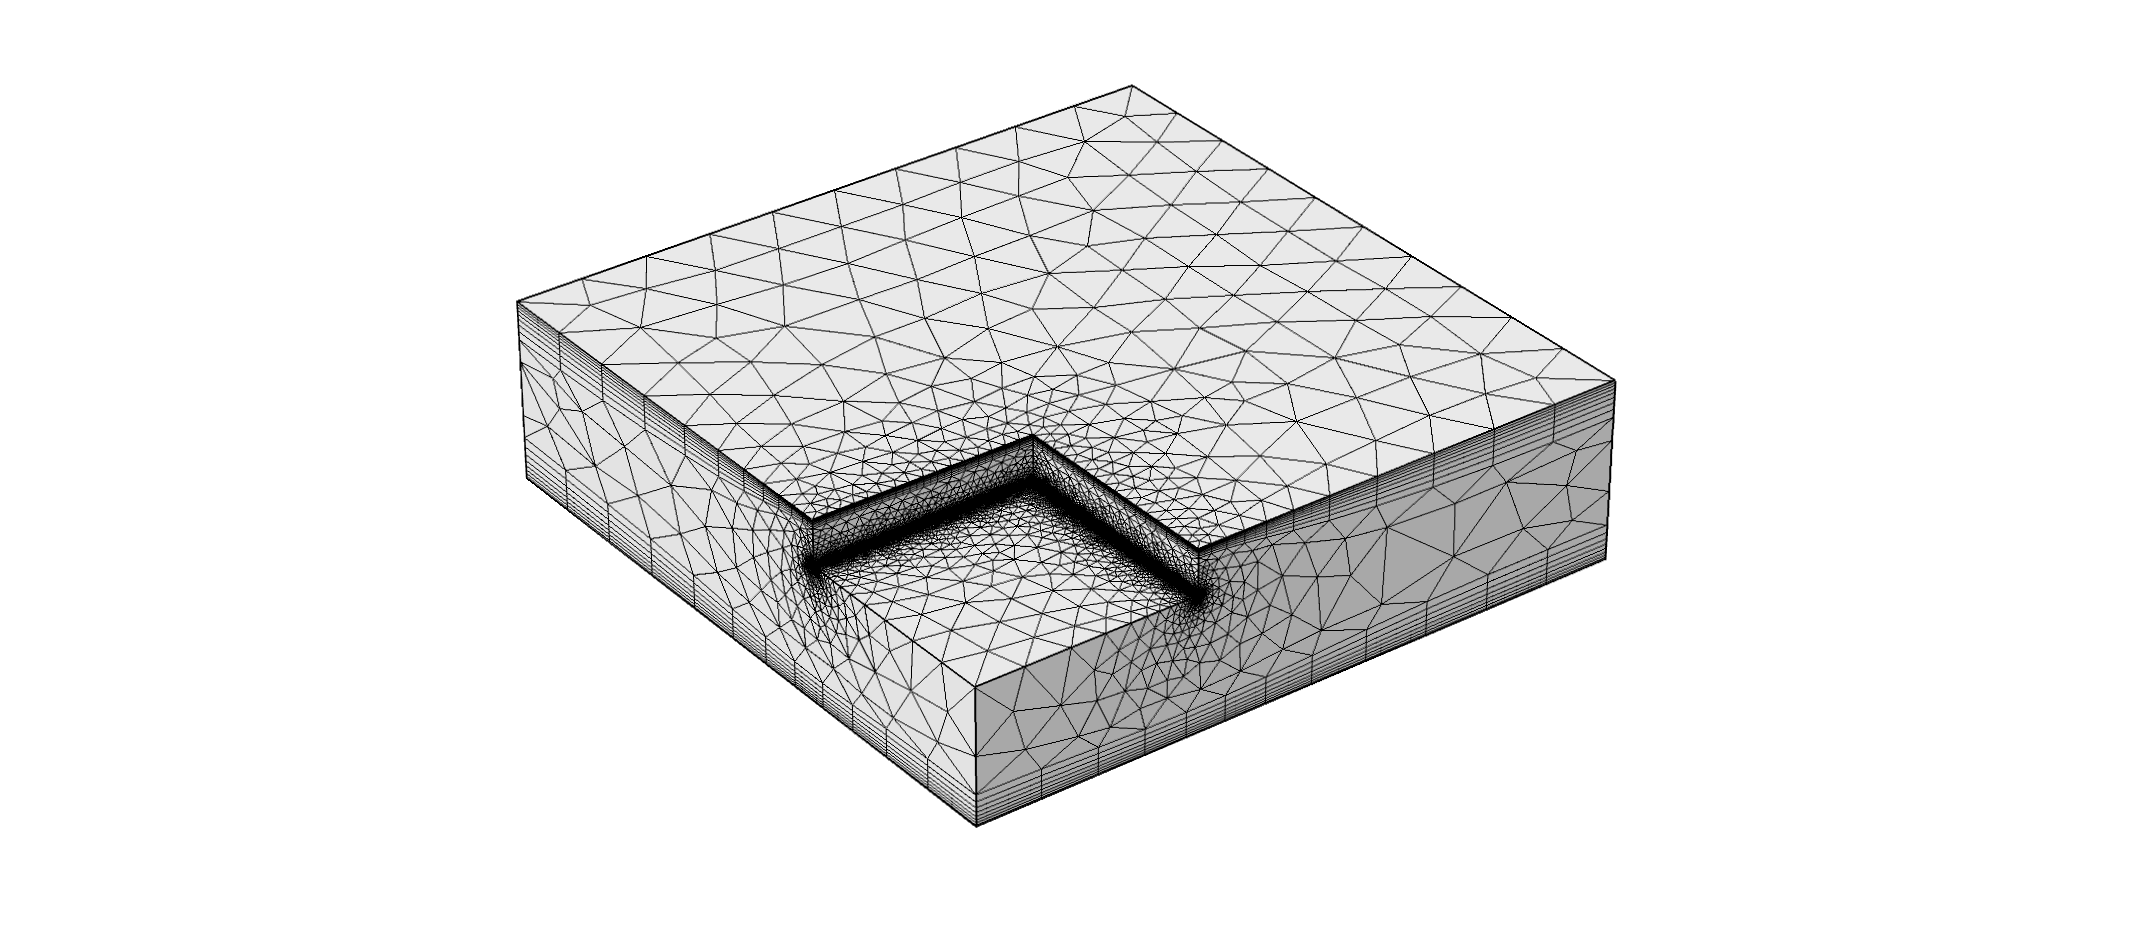
\includegraphics[width=0.75\textwidth]{meshed_model.png}
    \caption{The darker perimeter around the foundation highlights the higher mesh density along the foundation crack.}
    \label{fig:meshed_geometry}
  \end{subfigure}
  \begin{subfigure}[b]{\textwidth}
    \centering
    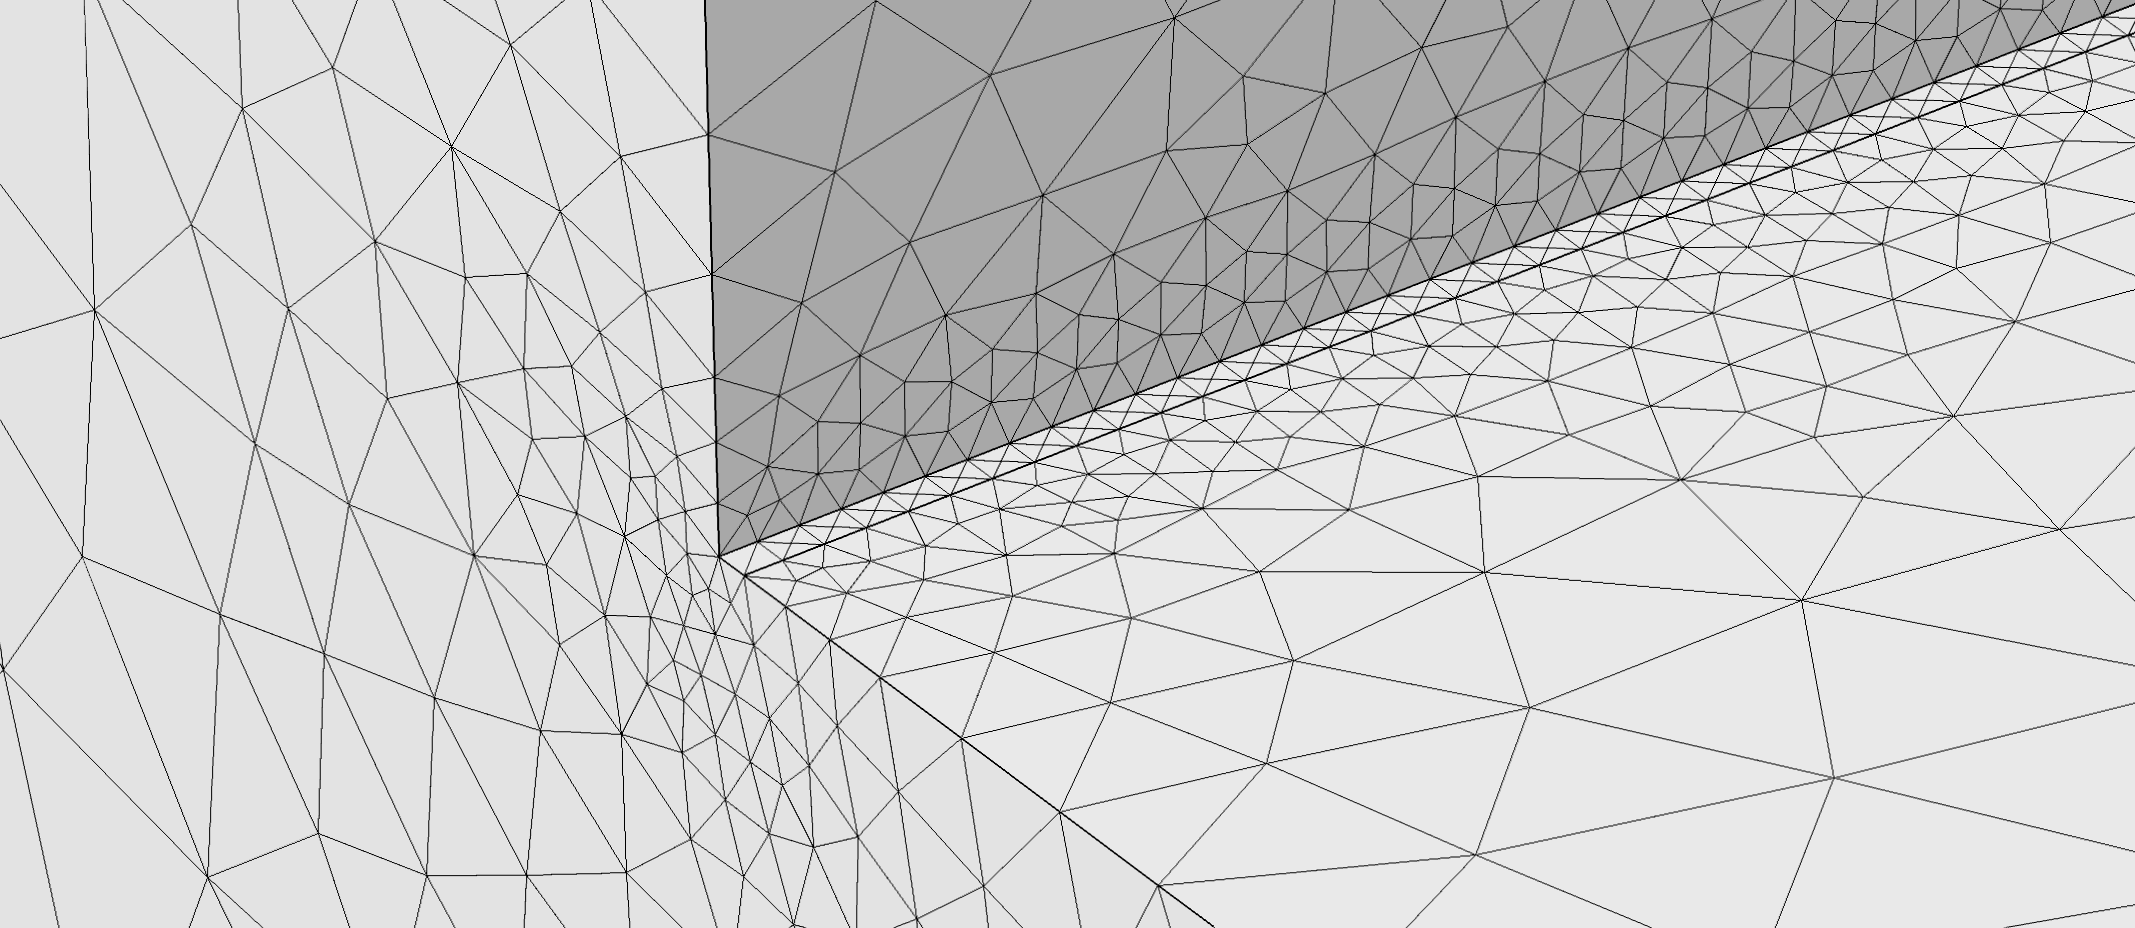
\includegraphics[width=0.75\textwidth]{mesh_crack.png}
    \caption{Close-up of the foundation crack mesh.}
    \label{fig:meshed_crack}
  \end{subfigure}
  \begin{subfigure}[b]{\textwidth}
    \centering
    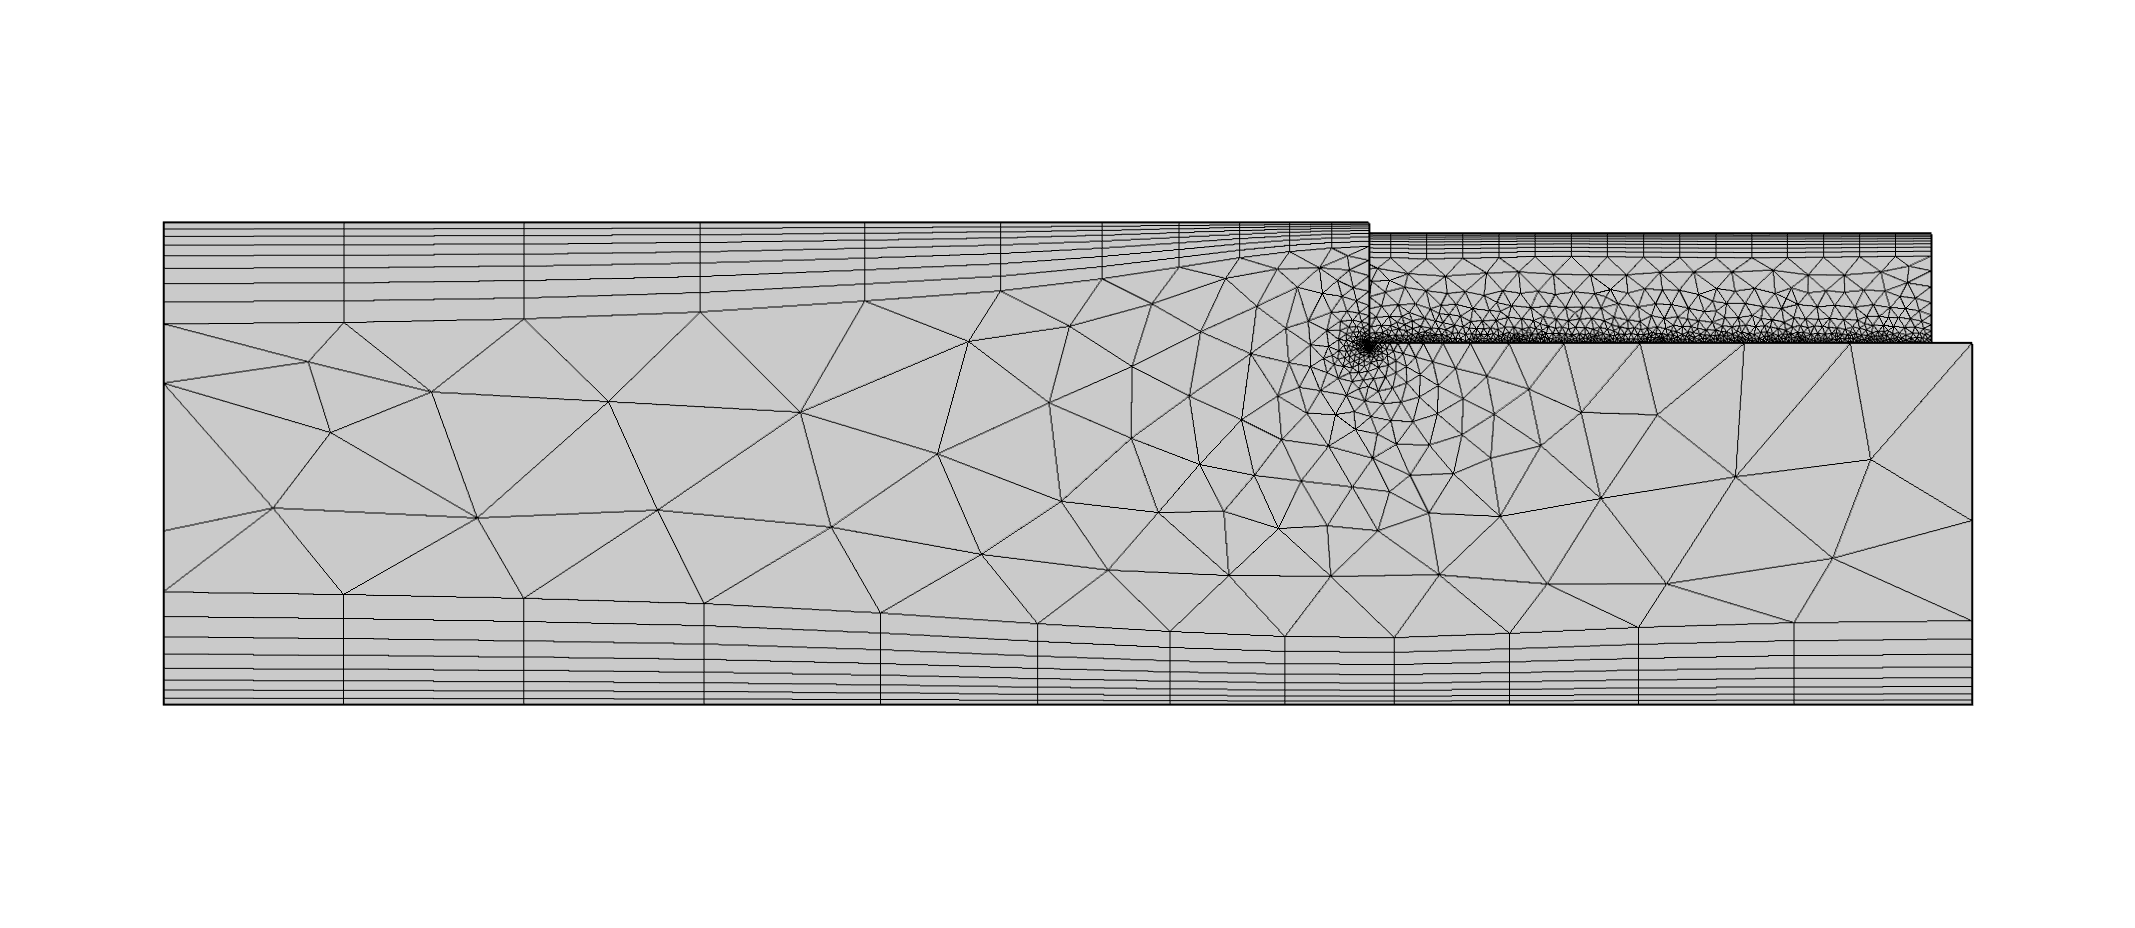
\includegraphics[width=0.75\textwidth]{mesh_boundary_layers.png}
    \caption{Side-view highlighting the boundary layer mesh.}
    \label{fig:mesh_boundary_layers}
  \end{subfigure}
  \caption[Initial finite element mesh of the modeled vapor intrusion scenario.]{Initial finite element mesh of the modeled vapor intrusion scenario.}
  \label{fig:mesh}
\end{figure}

\section{Solver Configuration}

A solver(s) is required to solve the VI model, and a few considerations need to be taken into account when choosing one.
For choosing and motivating a solver configuration, the \textit{COMSOL Multiphysics Reference Manual v5.3a}\cite{comsol_comsol_nodate} is here continuously used as a source.\par

For simplicity we will now first consider a stationary or steady-state problem.
Since our model is a multiphysics problem, i.e. many of the physical parameters depend on each other, we first need consider how to couple them.
They can be coupled by either using a \textit{segregated} or \textit{fully coupled} approach.\par

\paragraph{Segregated vs. fully coupled physics}

In a segregated solver, each governing equation is solved separately in a specific order.
For instance, in our VI example we can solve Darcy's Law first, get some solution for airflow in soil, and then use that velocity field in the transport equation, solve that, and then solve the indoor concentration equation, i.e. we solve one system equation per step.
These steps are simply iterated until convergence occurs in all of the separated steps.
In the case of VI calculations, the use of the segregated approach is fully justified because the concentrations of contaminant vapors are normally so low that they have no impact on the solution of soil airflow using Darcy's Law.
The fully coupled approach assembles a single large system of equations.
Both of these approaches should reach the same solution, but the fully coupled approach will do so faster, but at the expense of using more memory.\par

\paragraph{Direct vs. iterative solver}

Within each of these coupling approaches, we need to specify a solver to solve the system of equations.
Here we are again faced with a choice, and we could either use a \textit{direct} or \textit{iterative} solver.
Direct solvers, as the name implies, arrive at a solution directly and are based on LU-decomposition.
Iterative solvers on the other hand, iteratively approach the solution, and are based on conjugate gradient method.
The advantage of direct solvers is that they are faster, but use more memory, while iterative solvers are slower but use less memory.
In terms of choosing a solver algorithm, there are many options, but MUMPS and GMRES will be used as the respective algorithm for direct and iterative solvers.\par

\paragraph{Time-dependent solvers}

To solve a transient or time-dependent problem (which will be done in subsequent chapters) a solver to step forward in time is required.
Too large a time step will cause stability issues and ultimately convergence will be impossible, but obviously some discrete time step is required for a solution to be achievable.
A time-dependent solver picks an appropriate time-step and there are some popular approaches, such as using some high-order Runge-Kutta (RK) or backwards differentiation formula (BDF).
Regardless of the type of solver, for each time step the system of equations will be solved using one of the aforementioned solvers.
The difference between RK and BDF is that RK explicitly discretizes time while BDF does so implicitly.
In this work we will only use BDF as it is more stable than RK.\par

\paragraph{Choosing solvers}

The choice of solver will not affect (or should not at least) the solution to the problem.
However, it can have a large impact on computational time and resources, and these considerations dictate solver choice (this is also partially dependent on the mesh used, as this will affect memory usage too).
In this example, and throughout the models used in this work, we will favor speed over memory and therefore fully couple all our equations and use direct solvers.\par

\subsection{Adaptive Mesh Refinement}

The accuracy of the solution obtained by FEM is dependent on the quality of the mesh, something that was discussed in section \ref{sec:meshing}.
While the mesh designer can do much to create a mesh that performs well for the particular problem posed, refinement of the mesh is often needed and should be performed for every new model.\par

There are two types of mesh refinements in FEM.
The first type reduces the size of the elements and thereby the accuracy of the solution, this is called \textit{h-type} refinement ($h$ is often used to denote the mesh size).
The second increases the order of the polynomial of the basis function, called \textit{p-type} refinement which will likewise increases the solution accuracy.\par

h-type refinement is generally more attractive because it is simpler and the computational cost of p-type refinement increase faster than h-type.
However, p-types are useful if the user imports an already existing mesh, and is unable to change it, rendering h-type refinement impossible.
These two method can be combined to perform a \textit{hp-type} refinement.\par

Refinement is usually done by an algorithm, which is possible because FEM has the built-in ability to estimate the local error of the solution anywhere in the domain.
The downside with using an algorithm is that the user has little control over how the mesh is refined.
The user can also manually refine the mesh by solving the model and plot how some relevant metric converges as the mesh is refined.
This can be a very time consuming, and therefore algorithms are usually preferable; a hybrid solution is to manually alter the mesh after the algorithmic mesh refinement.\par

Refinement can either be done locally or globally.
Global refinement involves defining some singular metric that will be used to evaluate the quality of the mesh, e.g. one might use the total stress in a metal bar as a metric here.
In local refinement, one still has to define some metric for evaluating the quality of the refinement, but evaluation only occurs on a subset of the domain, e.g. the stress on just one boundary of the same metal bar.
In both approaches the elements that have the largest estimated local relative error are refined, but the exact details of the refinement can differ between specific refinement algorithms.
The local relative error is defined as the difference of the approximated solution $u_h$ from one mesh to another.
\begin{equation}\label{eq:rel_error}
  e = u_{h1} - u_h
\end{equation}
$e$ is the estimated local relative error (for every node);
$u_{h1}$ and $u_h$ are the approximated solutions on the refined and original meshes respectively.
The optimal type of refinement varies by problem, but a global refinement will generally be more computationally expensive.\par

\begin{figure}[htb!]
  \centering
  \begin{subfigure}[b]{\textwidth}
    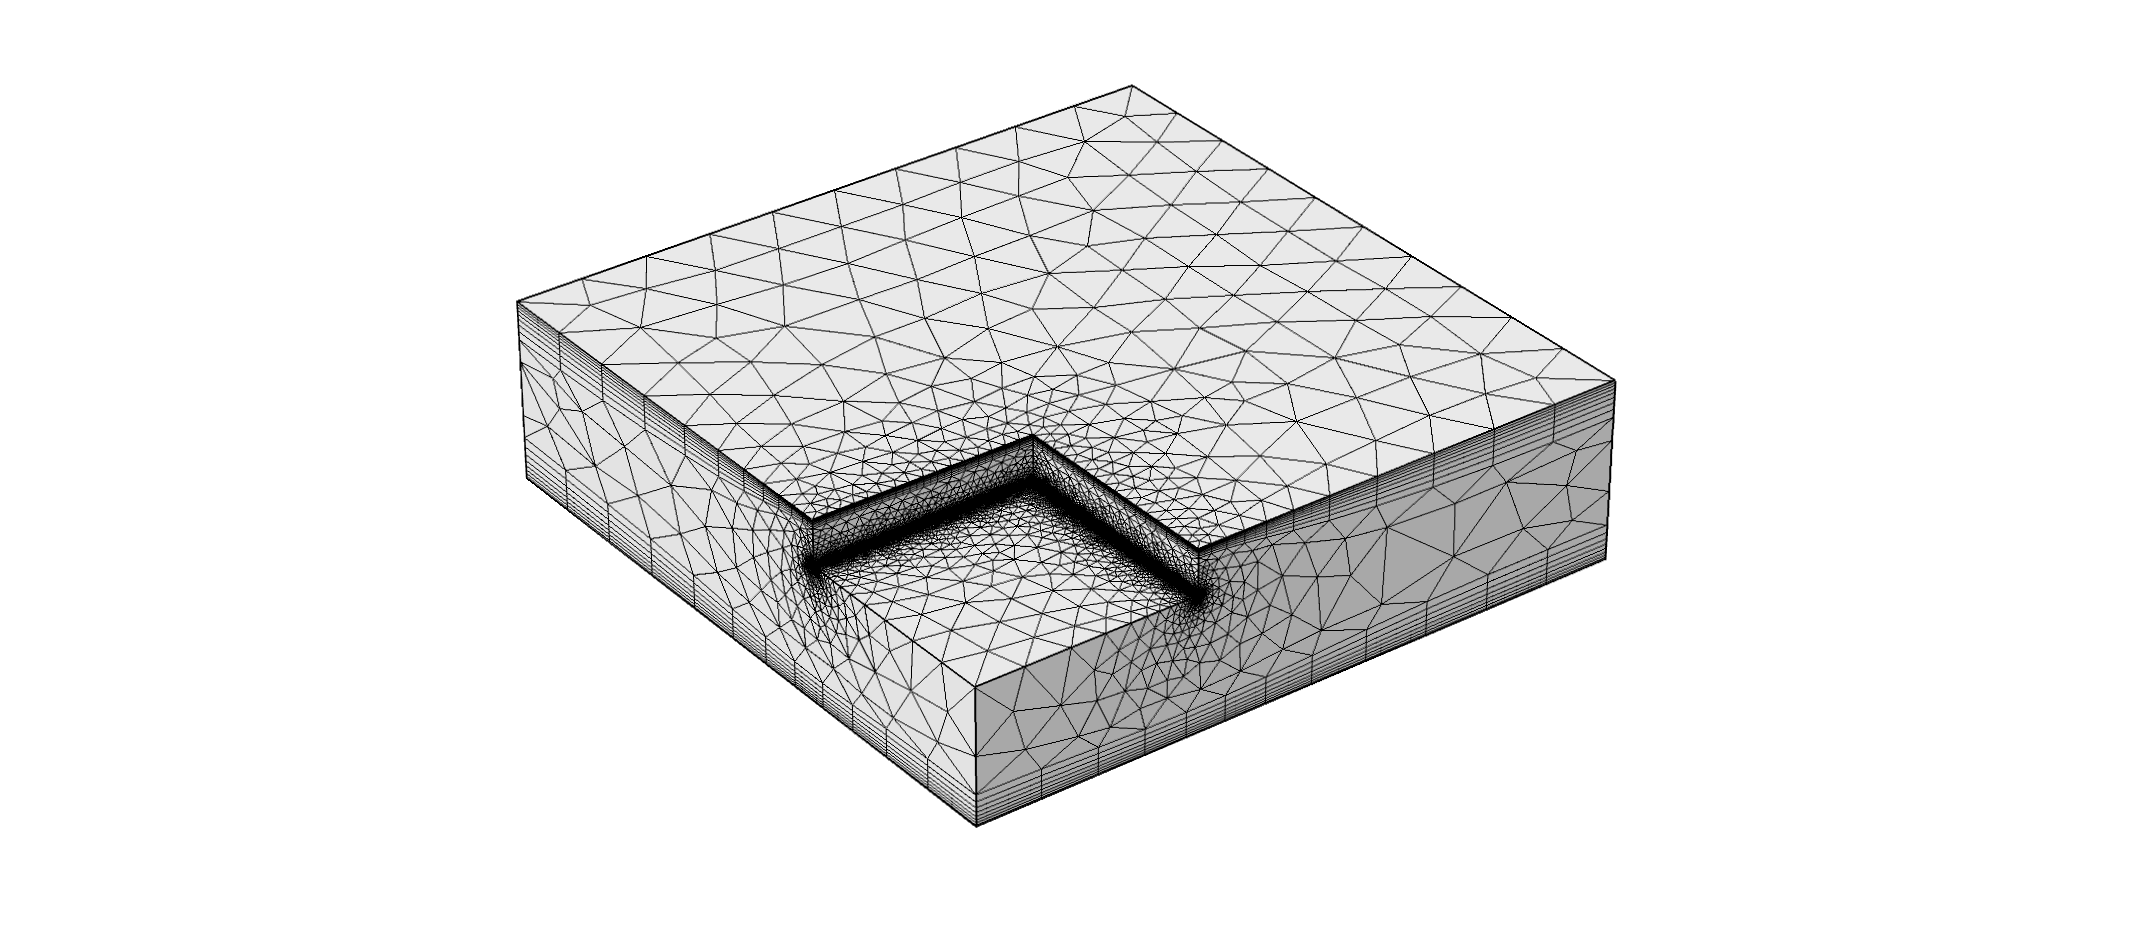
\includegraphics[width=\textwidth]{meshed_model.png}
    \caption{Original mesh. 362,657 elements.}
    \label{fig:mesh_before_refinement}
  \end{subfigure}
  \begin{subfigure}[b]{\textwidth}
    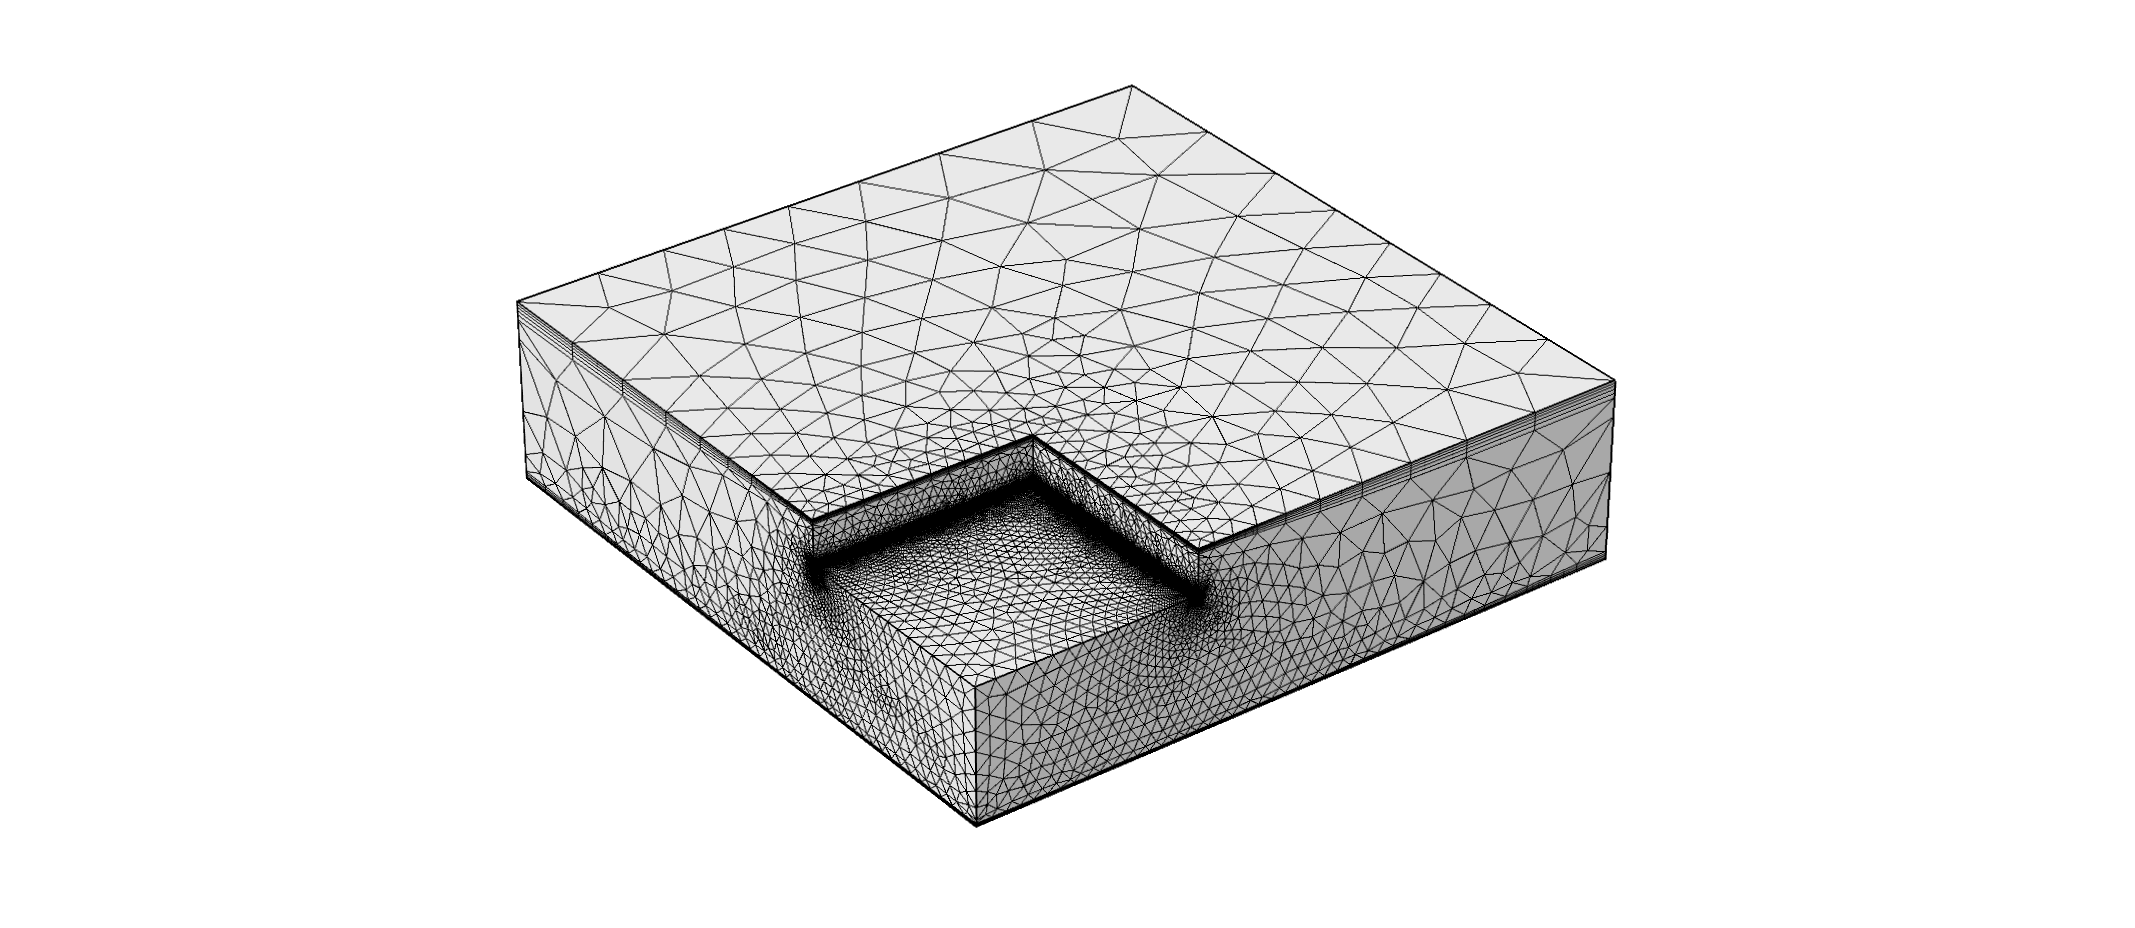
\includegraphics[width=\textwidth]{mesh_refined.png}
    \caption{Refined mesh after global refinement w.r.t. the indoor contaminant concentration. 1,065,743 elements.}
    \label{fig:mesh_after_refinement}
  \end{subfigure}
    \caption[Original and adaptatively refined mesh.]{Original and adaptatively refined mesh.}
    \label{fig:mesh_refinement_mesh}
\end{figure}

In this work we will use a global h-type refinement and use the indoor contaminant concentration $c_{in}$ as our refinement metric.
COMSOLs refinement algorithm has the nice ability to reinitialize the mesh, and can thereby coarsen elements, i.e. increase $h$ where the local error is very small.
This is handy as a fine mesh is not needed far away from the foundation crack - saving computational resources.
In this example we will tell the algorithm to refine the mesh three times, and stop if the total number of elements exceed 1 million, with a maximum coarsening factor of 3, and element growth rate of 1.3, i.e. the number of elements increase by roughly 70\% each iteration.\par

The result of this refinement can be seen in Figure \ref{fig:mesh_refinement_mesh} where the original and refined mesh are juxtaposed.
Notice how the mesh is now denser near the foundation, the boundary layers tighter (in particular near the groundwater boundary), and how the elements are larger in the periphery.
The original and refined meshes has 362,657 and 1,065,743 elements respectively.\par
Figure \ref{fig:mesh_refinement} shows how the value of $c_\mathrm{in}$ converges for each mesh refinement iteration.
What is plotted is the change in calculated indoor contaminant concentration with iteration.
Initially, very large changes are seen in the predicted values with the first iterations.
By the \nth{4} iteration, the improvements in estimates are getting very small.\par

\begin{figure}[htb!]
  \centering
  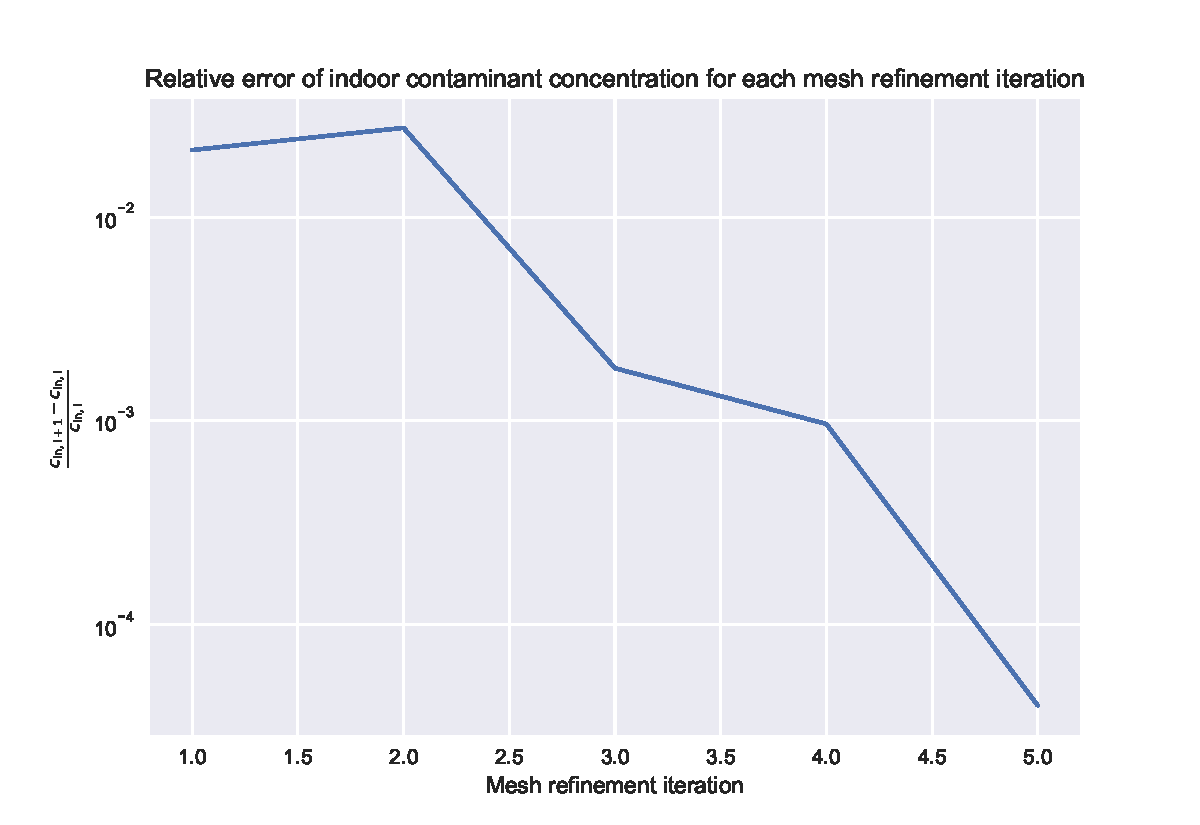
\includegraphics[width=0.75\textwidth]{mesh_refinement_error.pdf}
  \caption{Convergence of indoor air contaminant concentration as the mesh is refined.}
  \label{fig:mesh_refinement}
\end{figure}

\section{Post-processing \& Results}

One of the benefits of using a FEM software like COMSOL is its advanced post-processing capabilities.
This allows the user to examine the physics driving VI in great detail.
Figure \ref{fig:model_pressure} shows the resulting pressure field from solving Darcy's Law, as well as the associated airflow streamlines in the soil.
Here we see the pressure in the near foundation crack region is roughly the same as the house pressurization of \SI{-5}{\pascal}, which quickly decreases towards the ground surface.
It is also apparent how this pressure field induces a airflow from the ground surface, with air near the house heading relatively straight to the foundation crack, whereas the air further away from the house penetrates deeper into the soil and almost "whirlwinds" underneath the house.\par

\begin{figure}[htb!]
  \centering
  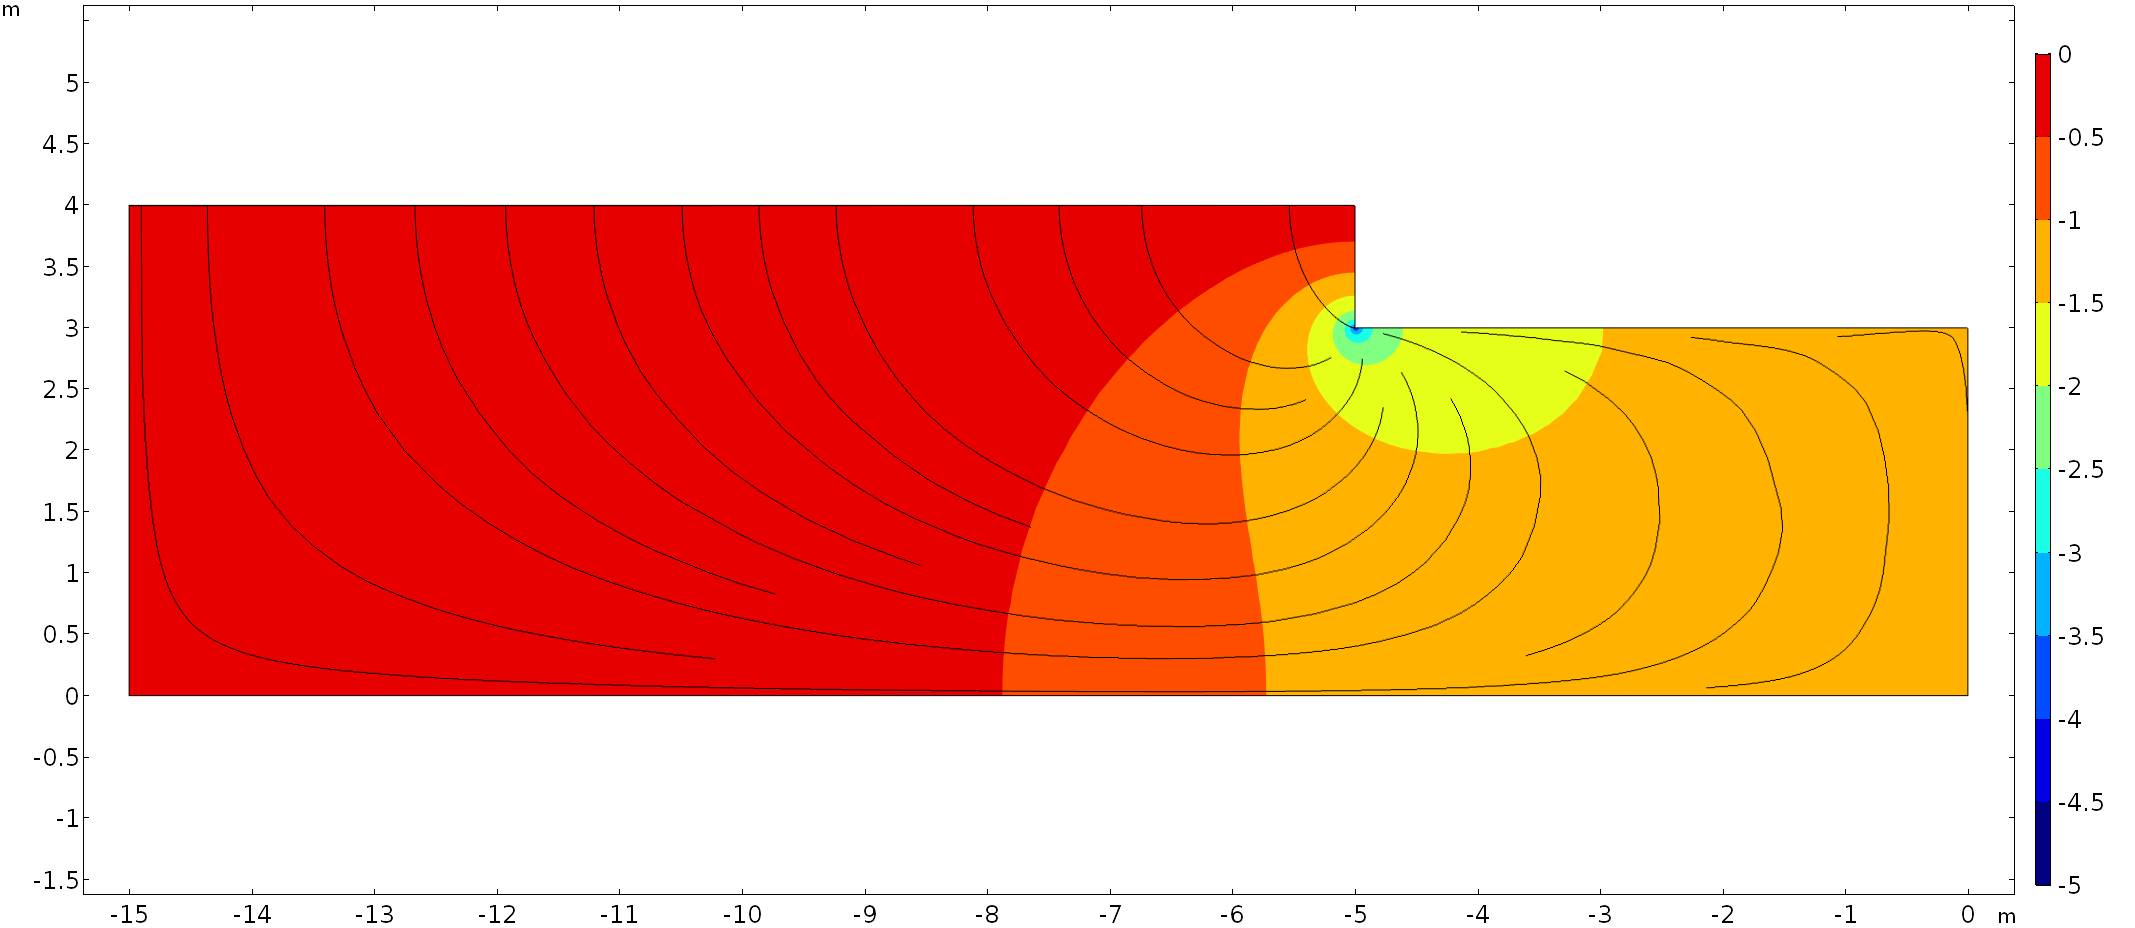
\includegraphics[width=0.75\textwidth]{model_pressure.png}
  \caption{Pressure field from Darcy's Law with associated airflow streamlines.}
  \label{fig:model_pressure}
\end{figure}

\begin{figure}[htb!]
  \centering
  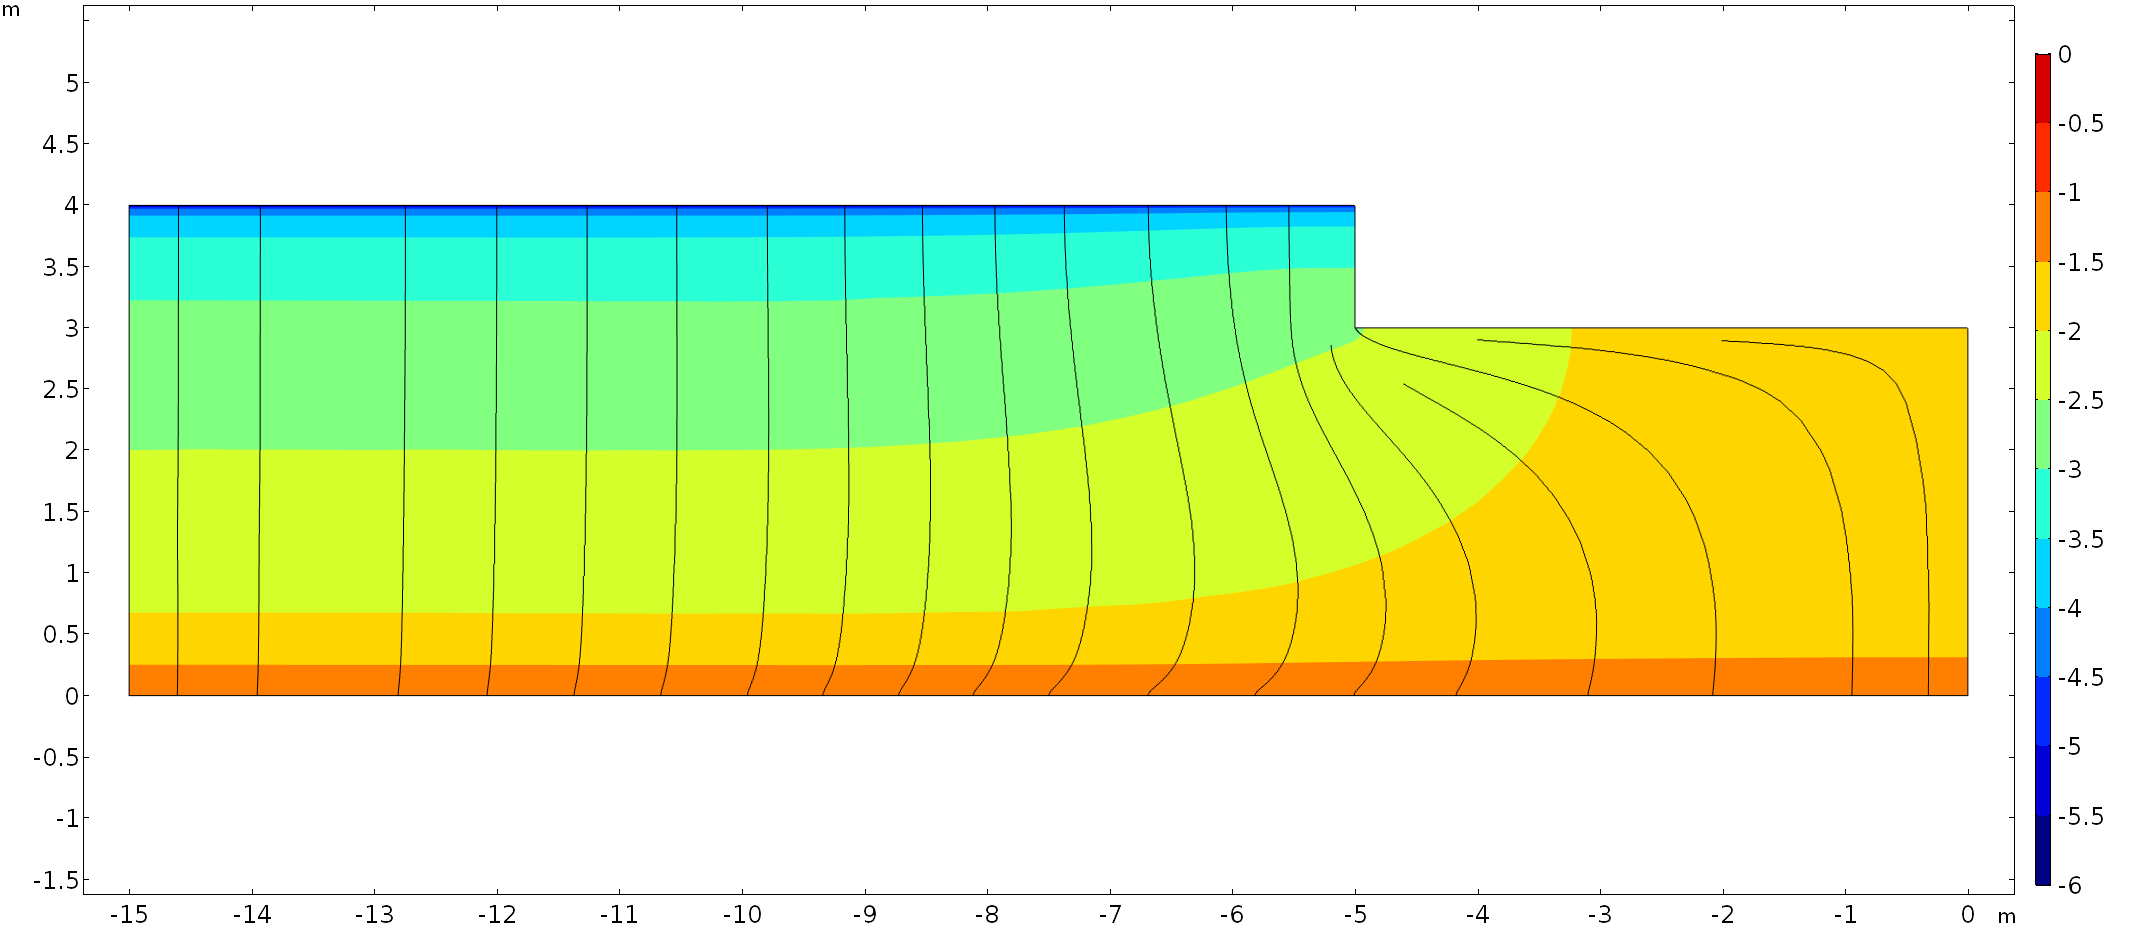
\includegraphics[width=0.75\textwidth]{model_concentration.png}
  \caption{Contaminant concentration in the soil, normalized to groundwater concentration and log-transformed, with transport streamlines.}
  \label{fig:model_concentration}
\end{figure}

The contaminant concentration in the soil, normalized to the groundwater source concentration and log-transformed, with the contaminant flux streamlines, is examined in Figure \ref{fig:model_concentration}.
Here see that far away from the house, the contaminant vapor simply diffuse straight from the groundwater source to the atmosphere, while these accumulate underneath the house, which acts as a diffusion blocker.
Based on those streamlines we can conclude that the advective component of the flux is very here small.
Perhaps surprisingly, we do not see a significant advective transport downwards along the wall of the house.
However, considering that the soil type is sandy loam, airflow velocities are expected to be small.\par

One might think that advective transport is large in the horizontal direction along the foundation slab, as the transport and airflow streamlines are so similar.
However, by inspecting Figure \ref{fig:model_velocity_crack} we see that airflow velocities are not greater here than elsewhere, and therefore the advective transport is not either.
To make sense of this, we can inspect the horizontal diffusive flux, divided by the magnitude of the total flux
\begin{equation}
  \frac{j_\mathrm{diff,y-direction}}{|j_\mathrm{total}|}
\end{equation}
to see what portion of the total transport the diffusive horizontal represents here.
The results of this is shown in Figure \ref{fig:model_horizontal_diff}, where see that the horizontal diffusive flux in the left direction accounts for 80\% of the total flux magnitude, as indicated by -0.8. % TODO Explain this better
This shows the power of modeling and how it can reveal things that at first seem intuitively correct, but in fact are not.\par

\begin{figure}[htb!]
  \centering
  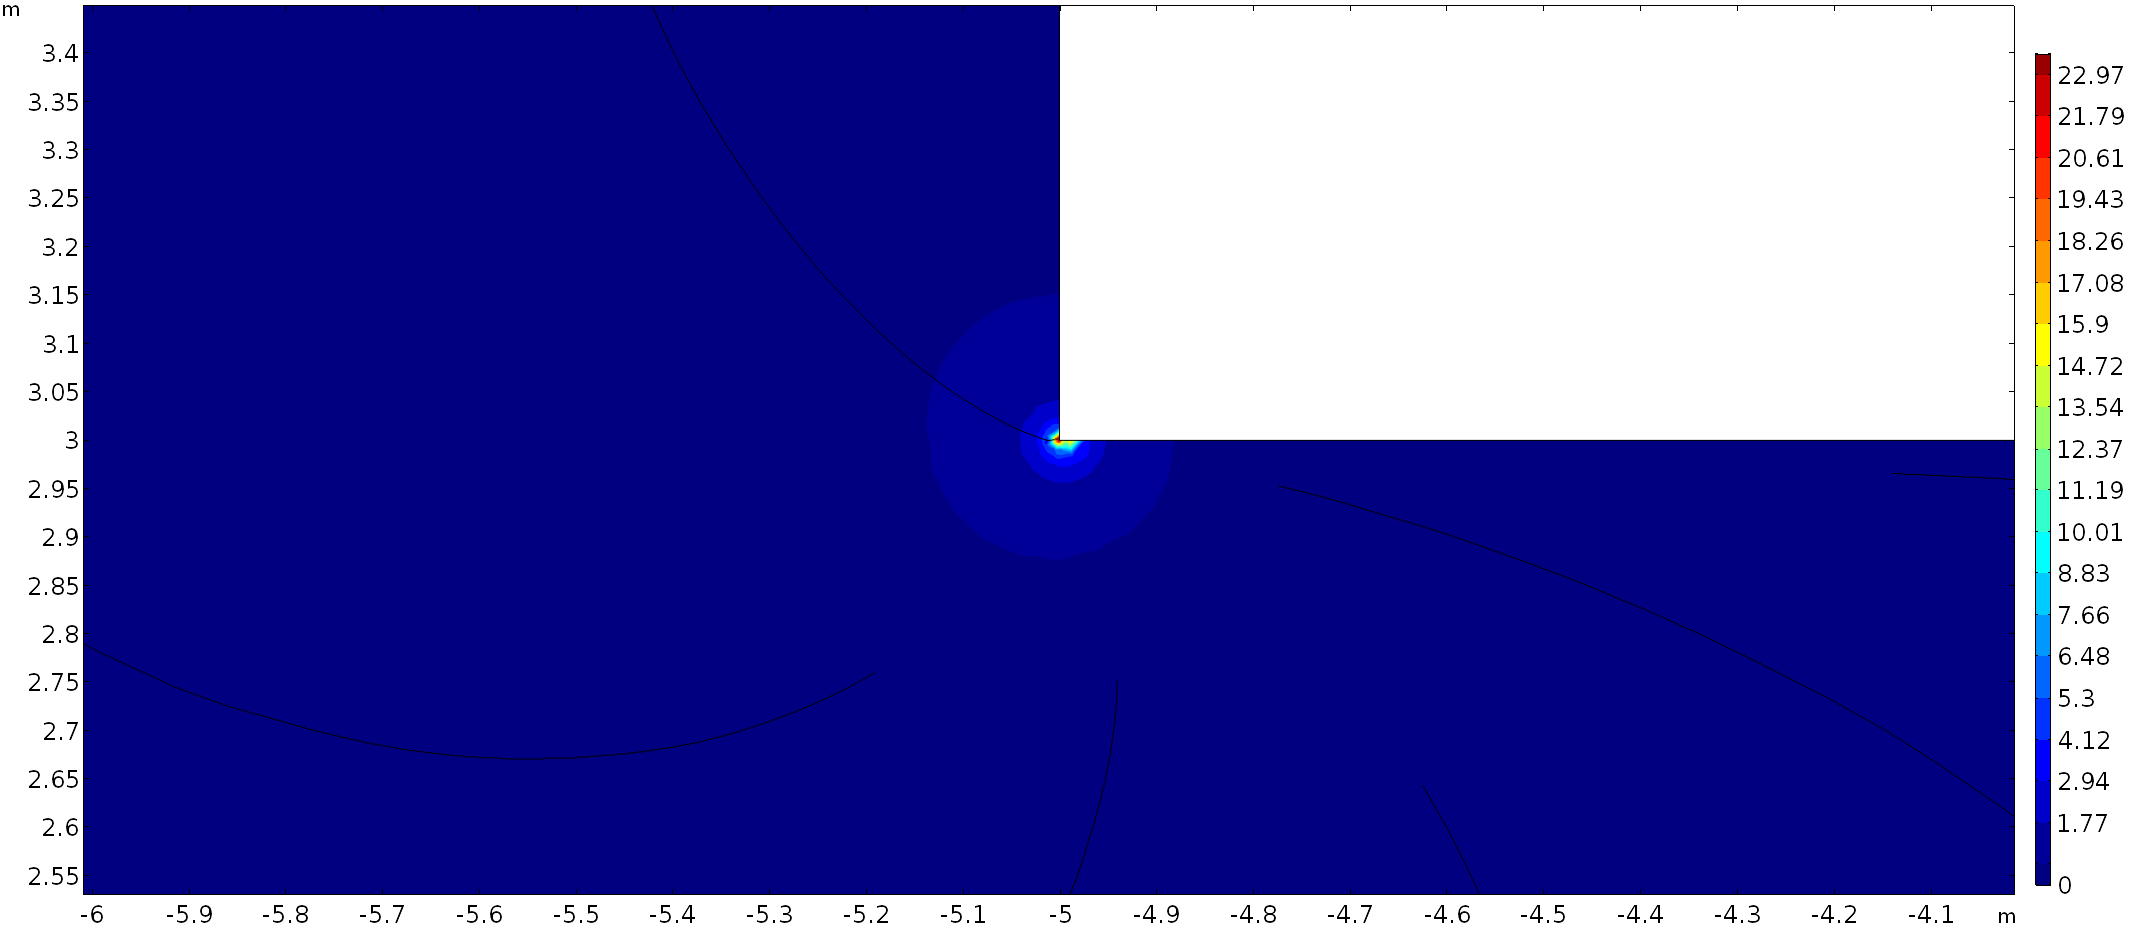
\includegraphics[width=0.75\textwidth]{model_velocity_crack.png}
  \caption{Airflow velocity [\si{\milli\metre\per\hour}] near the foundation crack with associated its streamlines.}
  \label{fig:model_velocity_crack}
\end{figure}

\begin{figure}[htb!]
  \centering
  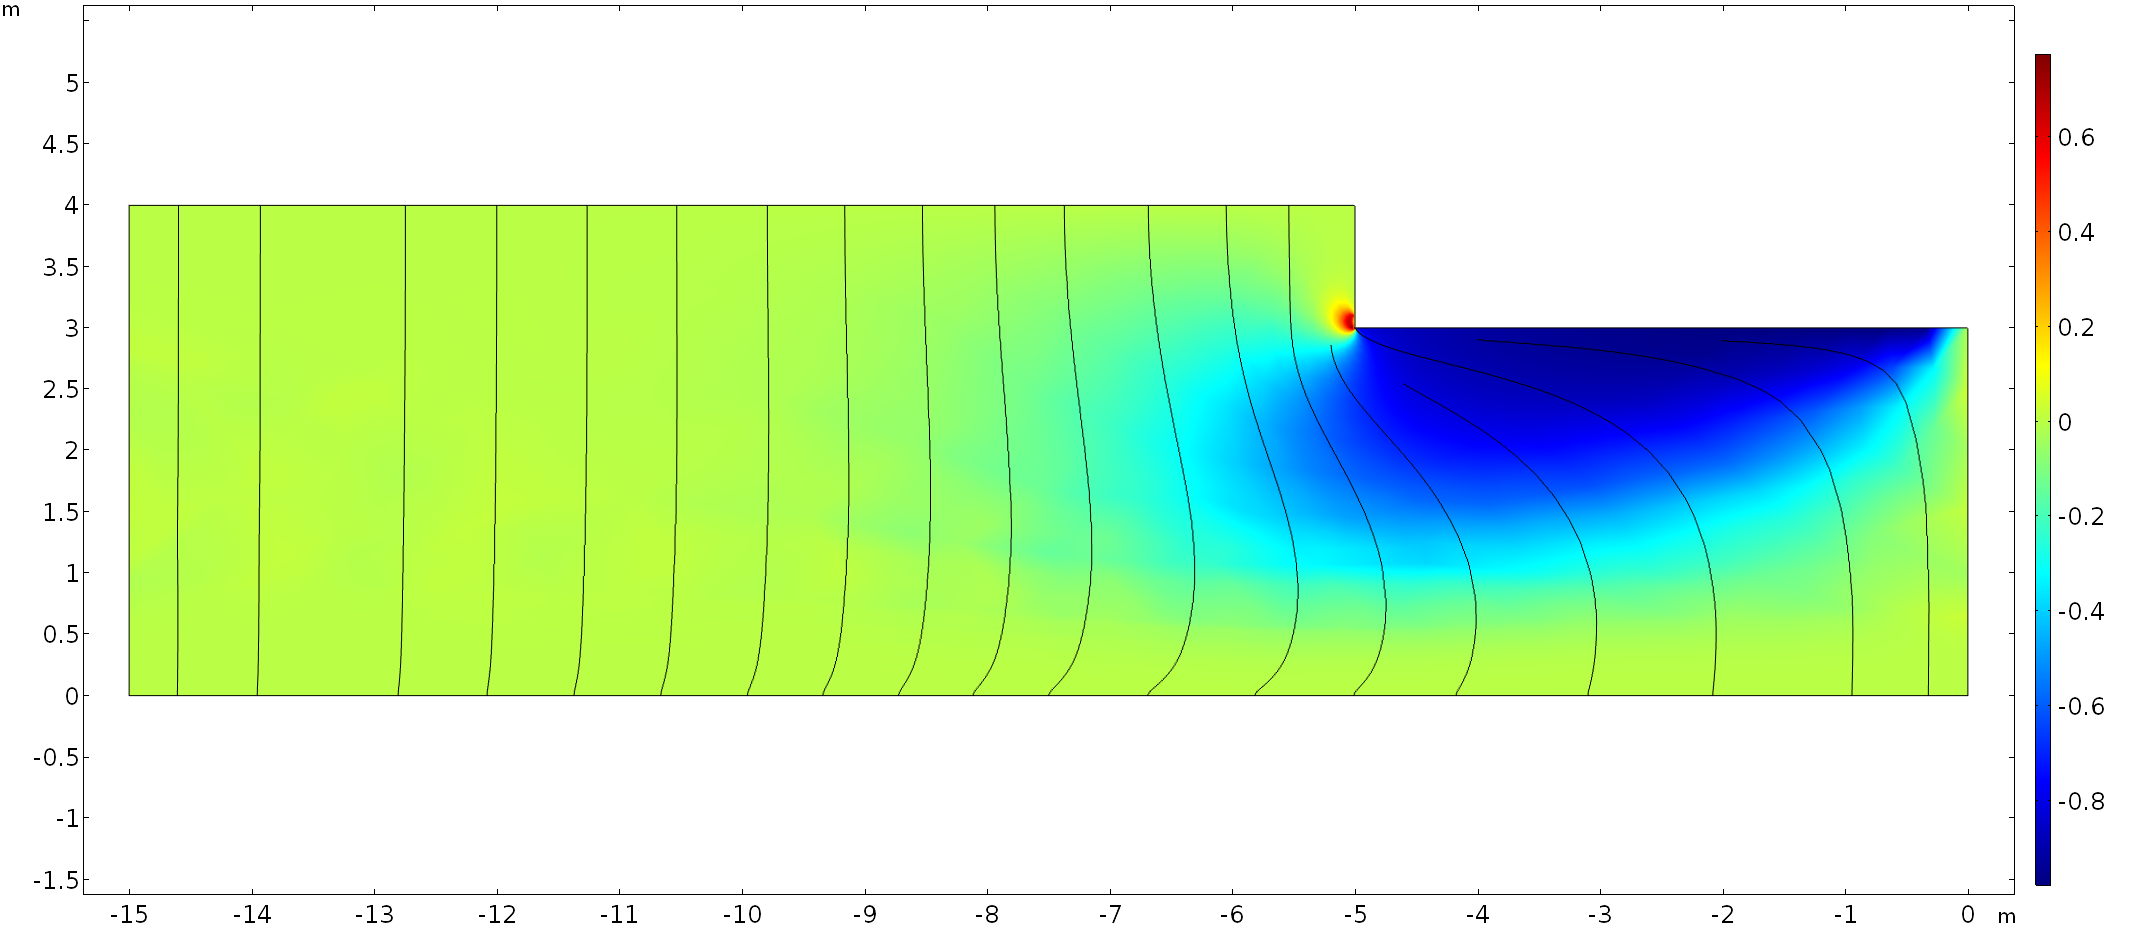
\includegraphics[width=0.75\textwidth]{model_transport_flux_y.png}
  \caption{Horizontal diffusive flux component of the magnitude of the total flux. 1 here would indicates that all of the contaminant transport is due to diffusion, and occurs solely in the rightwards direction.}
  \label{fig:model_horizontal_diff}
\end{figure}

Another useful feature of post-processing is that it can be used for bug searching and to evaluate where the mesh can be potentially improved.
When the transport equation is used to numerically model contaminant transport, there is a tendency for the solution to oscillate around the "true" solution, and thereby violate mass conservation, if the mesh size in a particular element is too large.
This can be quantified by the cell Péclet number, which characterizes the relative magnitude of advection/diffusion in a cell.
\begin{equation}
  \mathrm{Pe_{cell}} = \frac{\mathrm{adv_{cell}}}{\mathrm{diff_{cell}}} = \frac{u_g h}{2 D_\mathrm{eff}}
\end{equation}
here $u_g$ [\si{\metre\per\second}] is the soil-gas airflow velocity;
$h$ [\si{\metre}] is the mesh size in the element or cell;
and $D_\mathrm{eff}$ [\si{\metre\squared\per\second}] is the effective diffusivity in the cell.
If $\mathrm{Pe_{cell}} > 1$ there is a risk that this oscillating behavior will manifest.
Small exceedances, $~\mathrm{Pe_{cell}} < 25$, are usually mitigated by various stabilization schemes, which are inherently integrated into COMSOL as well as many other FEM packages, but for larger values further mesh refinement may be required.\par

Figure \ref{fig:model_cell_peclet} shows $\mathrm{Pe_{cell}}$ as a volume plot, and excludes all values that fall below one.
As we can see, only the region close to the groundwater exceeds $\mathrm{Pe_{cell}}$, which is due to the very small $D_\mathrm{eff}$ there.
The exceedance is small, so the stabilization scheme is able to compensate which is confirmed by Figure \ref{fig:model_concentration} (no oscillations visible).
This is also a region where even if such oscillations occurred, would probably not affect the indoor contaminant concentration.
Regardless, Figure \ref{fig:model_cell_peclet} shows where the mesh may potentially be refined, which comes in handy to know if one runs a model where airflow velocities are significantly higher than in this example.\par

\begin{figure}[htb!]
  \centering
  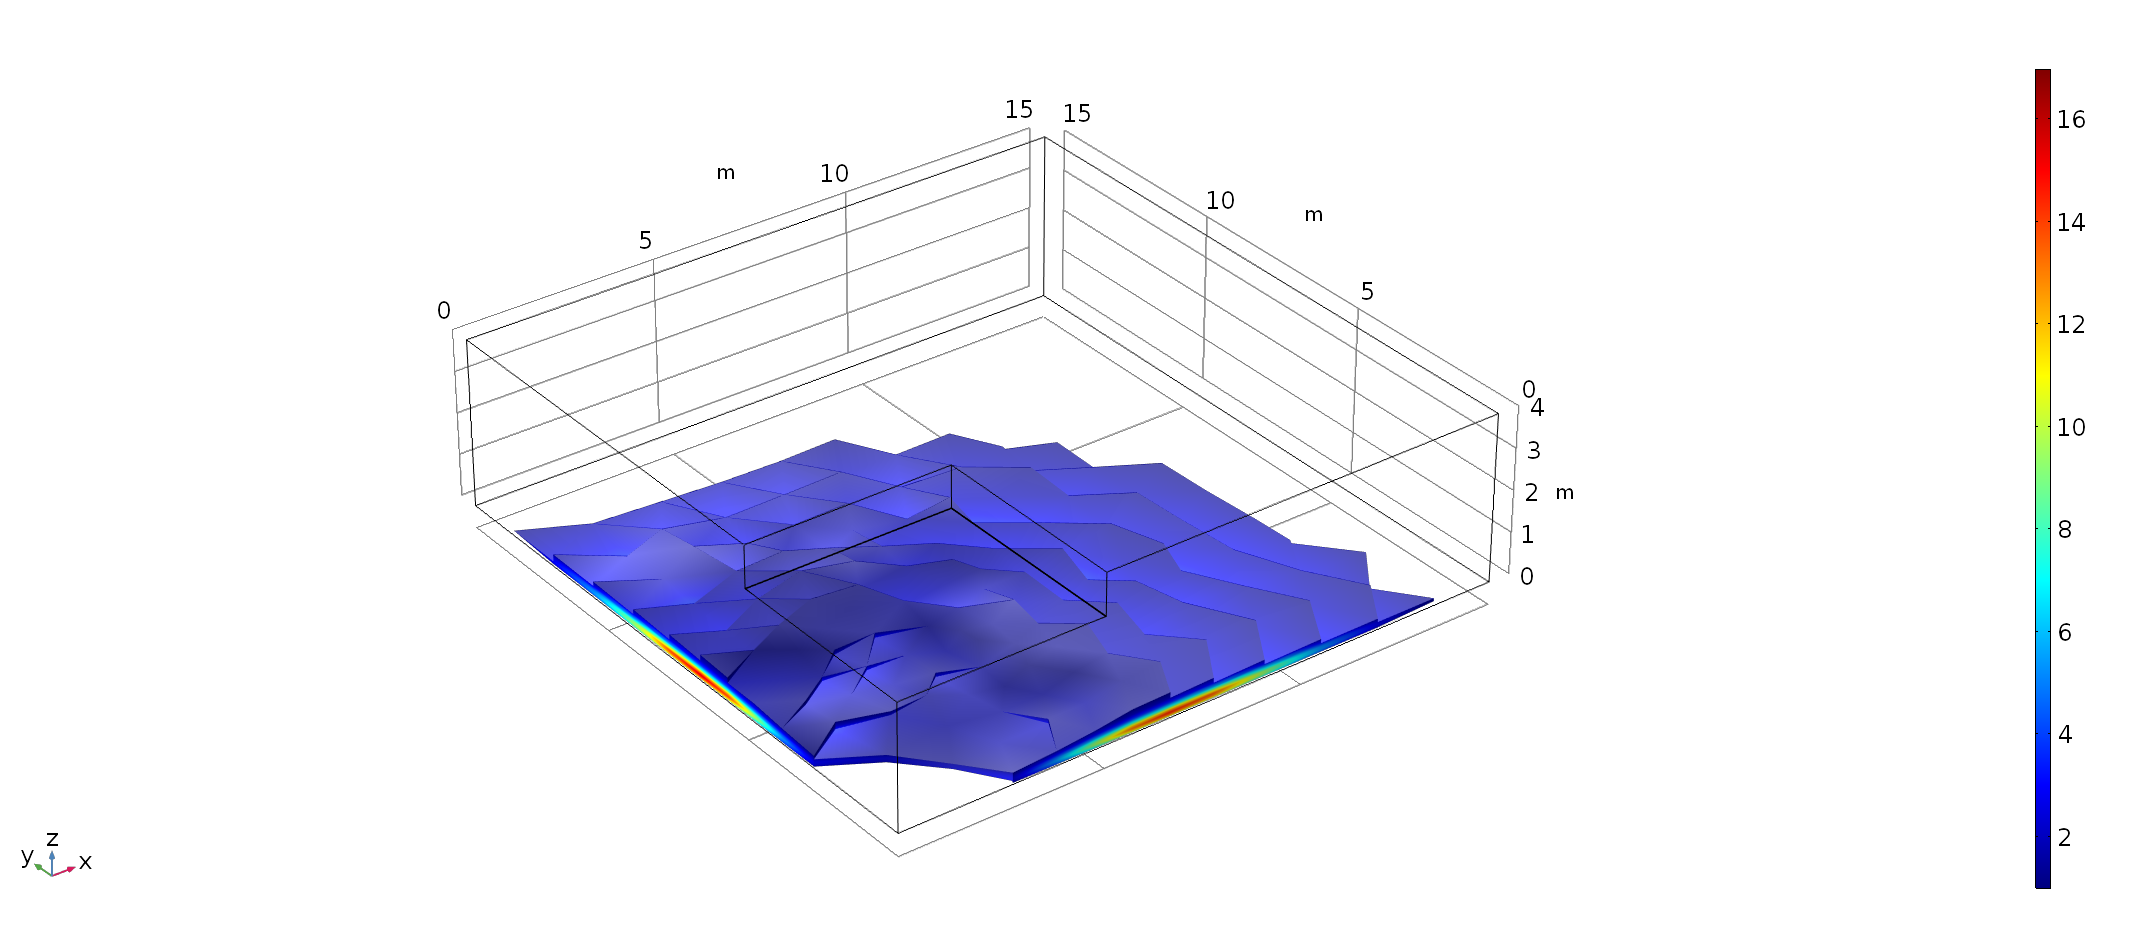
\includegraphics[width=0.75\textwidth]{model_cell_peclet.png}
  \caption{Volume plot showing where the cell Péclet number exceeds 1 and its actual value. I.e. it suggests where the mesh may be improved.}
  \label{fig:model_cell_peclet}
\end{figure}


\appendix
\clearpage
\begin{appendices}

  \section{Geometry Generation}

  To create our quarter geometry, only a few simple geometric objects and Boolean operations are required: two cuboids, two rectangles, one Boolean difference operation, and one Boolean join operation.
  Figure \ref{fig:geometry} shows the resulting geometry.
  Note that $z = \SI{0}{\metre}$ is the groundwater/soil interface and the plane of symmetry is around the $(x, y) = (\SI{0}{\metre},\SI{0}{\metre})$ axis\par

  To create the soil surrounding the building using the COMSOL geometry generator:
  \begin{enumerate}
    \item Create a \SI{15}{\metre} by \SI{15}{\metre} by \SI{4}{\metre} block with its base at $(x, y, z) = (\SI{0}{\metre},\SI{0}{\metre},\SI{0}{\metre})$. This is the entire soil domain.
    \item Create a \SI{5}{\metre} by \SI{5}{\metre} by \SI{1}{\metre} block with its base at $(x, y, z) = (\SI{0}{\metre},\SI{0}{\metre},\SI{3}{\metre})$. This will represent the volume that the house take up in the soil, i.e. the underground portion of the basement.
    \item Perform a difference operation, removing the "basement" block from the "soil" block.
  \end{enumerate}
  At this point you will see that a quarter soil domain has been created, with an empty space that represents a house with a foundation slab located \SI{1}{\metre} bgs.\par

  The foundation crack will be modeled by joining two  \SI{1}{\centi\metre} wide strip that spans the perimeter of the surface that represents the house foundation.
  This strip is created by joining two rectangles on foundation surface:
  \begin{enumerate}
    \item Define a work plane \SI{3}{\metre} above zero. This allows us to place two-dimensional objects on the surface of or inside a three-dimensional object.
    \item On the work plane create a \SI{5}{\metre} by \SI{1}{\centi\metre} rectangle with its base at $(x, y) = (\SI{0}{\metre},\SI{5}{\metre} - \SI{1}{\centi\metre})$. This represents one side of the perimeter crack.
    \item Copy the rectangle and rotate it \SI{90}{\degree} around the corner of the foundation, i.e. $(x, y) = (\SI{5}{\metre} - \SI{0.5}{\centi\metre},\SI{5}{\metre} - \SI{0.5}{\centi\metre})$.
    \item Join the two rectangles to create a unified perimeter foundation crack.
  \end{enumerate}
  Now the geometry of this VI scenario is complete.\par

  \section{Properties}
  % TODO: Make sure gravel density data is correct
  % TODO: Flip the table?
  \begin{table}
    \centering
    \caption{Properties and van Genuchten parameters of select soil types\cite{abreu_conceptual_2012}.}
    \label{tbl:soils}
  \begin{tabular}{c c c c c c c}
    \toprule
    \multirow{2}{*}{Soil type} & Permeability & Density & Porosity & Residual moisture & \multicolumn{2}{c}{van Genuchten parameters} \\
    & $\kappa \; \mathrm{(m^2)}$ & $\rho \; \mathrm{(kg/m^3)}$ & $\theta_t$ & $\theta_r$ & $\alpha$ & $m$ \\
    \hline
    Sand & \num{9.9e-12} & 1430 & 0.38 & \num{5.3e-2} & 3.5 & 3.2 \\
    Loamy sand  & \num{1.6e-12} & 1430 & 0.39 & \num{4.9e-2} & 3.5 & 1.7 \\
    Sandy loam  & \num{5.9e-13}  & 1460 & 0.39 & \num{3.9e-2} & 2.7 & 1.4 \\
    Sandy clay loam  & \num{2.0e-13} & 1430 & 0.38 & \num{6.3e-2} & 2.1 & 1.3 \\
    Loam  & \num{1.9e-13}& 1380 & 0.40 & \num{6.1e-2} & 1.5 & 1.5 \\
    Silt loam  & \num{2.8e-13} & 1380 & 0.44 & \num{6.5e-2} & 0.51 & 1.7 \\
    Clay loam  & \num{1.3e-13}  & 1500 & 0.44 & \num{7.9e-2} & 1.6 & 1.4 \\
    Silty clay loam & \num{1.7e-13} & 1390 & 0.48 & \num{9.0e-2} & 0.84 & 1.5 \\
    Silty clay  & \num{1.5e-13} & 1300 & 0.48 & \num{1.1e-1} & 1.6 & 1.3 \\
    Silt  & \num{6.7e-13} & 1260 & 0.49 & \num{5.0e-2} & 0.66 & 1.7 \\
    Sandy clay  & \num{1.7e-13} & 1470 & 0.39 & \num{1.2e-1} & 3.3 & 1.2 \\
    Clay  & \num{2.3e-13} & 1330 & 0.46 & \num{9.8e-2} & 1.3 & 1.3 \\
    Gravel\cite{dan_capillary_2012} & \num{1.3e-9} & 1430 & 0.42 & \num{5.0e-3} & 100 & 2.19 \\
    \bottomrule
  \end{tabular}
  \end{table}
\end{appendices}


\section{Introduction}

To formulate a mathematical description of VI, we consider a simple hypothetical VI scenario at steady-state and develop a three-dimensional model of this.
Consider a VI impacted house with a \SI{10}{\metre} by \SI{10}{\metre} foundation footprint with a basement whose foundation lies \SI{1}{\metre} below ground surface (bgs).
There is also a \SI{1}{\centi\metre} wide crack along the perimeter of the \SI{15}{\centi\metre} thick foundation slab, where all contaminant vapor entry into the house is assumed to occur.
Here we will consider the basement alone as the control volume for which the indoor contaminant concentration will be determined.
It is assumed to have a ceiling height of \SI{3}{\metre}, giving a total volume of \SI{300}{\metre\cubed}
and that contaminant vapors are expelled via air exchange with the exterior of the house; the air exchange rate with outdoor air is assumed to be \SI{0.5}{\per\hour}.\par

The contaminant source be the underlying groundwater, which is assumed to be \SI{4}{\metre} bgs, and it is infinitely and homogenously contaminated with TCE (we will normalize everything to this source concentration, so the value does not matter), i.e. the groundwater contaminant concentration does not change over time nor does it have any concentration gradients.
We will only consider contaminant transport in the portion of soil between the open ground surface and the groundwater interface - the \textit{vadose zone}.
This soil is assumed to be homogenous and consist only of \textit{sandy loam} type soil, i.e. there no soil layers, rocks, etc.
For now, we will assume that no contaminant sorption into/onto the soil occurs, but this phenomena will be explored in Chapter (TBD).% TODO: Sorption chapter reference
The house is assumed to be surrounded by open ground that extend \SI{10}{\metre} from the house wall.
Contaminant concentration in the atmosphere is assumed so low that is effectively zero, i.e. contaminant vapors that reach the ground surface are immediately infinitely diluted. \par

The house interior is assumed to be slightly depressurized relative to ambient due to the stack effect; the indoor/outdoor pressure difference is \SI{-5}{\pascal}
This induces an airflow from the ground surface, through the soil, and into the house via the foundation crack.
The airflow interacts with contaminant diffusion in the soil.
Figure \ref{fig:vi_scenario} shows a figure summarizing this VI scenario.\par

% TODO Add a basement to the picture
\begin{figure}
  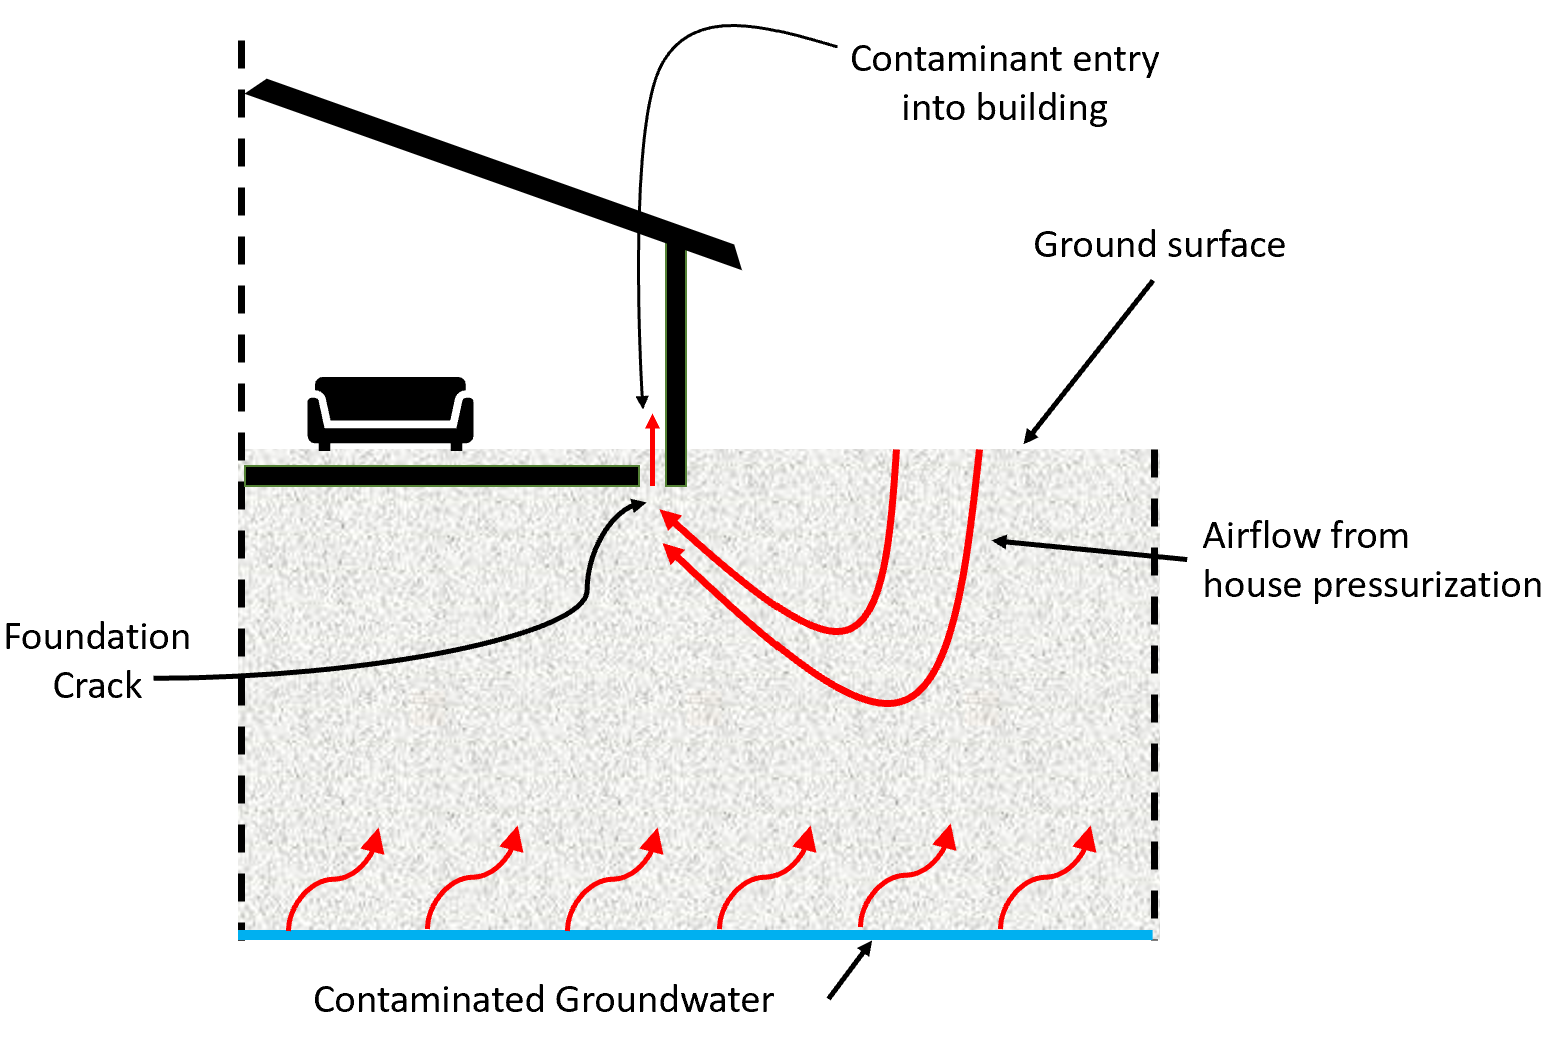
\includegraphics[width=\textwidth]{model_cartoon.png}
  \caption{The considered VI scenario.}
  \label{fig:vi_scenario}
\end{figure}

The basement interior will be modeled as a continuously stirred tank reactor (CSTR), (but without reactions), where the indoor contaminant concentration will depend on the contaminant entry rate $n_\mathrm{ck}$ from the soil via the foundation crack and the air exchange rate $A_e$.
The details of this will be covered section \ref{sec:indoor}.\par

To determine $n_\mathrm{ck}$ the contaminant transport in the soil needs to be modeled.
This will be done using the advection-diffusion equation, which will be modified for transport in soils.
The contaminant transport itself is driven by a concentration gradient and airflow in the soil.
The contaminant source (groundwater) and sink (atmosphere and contaminant entry into the building) will largely determine the concentration gradient, while the airflow needs to be calculated separately.\par

The airflow in the soil is modeled by Darcy's Law, and is driven by a pressure gradient in the soil, which induced by the indoor/outdoor pressure difference.
Details are in section \ref{sec:darcys_law}.\par

One last consideration is that the vadose zone is partially saturated with water, with the soil pores more or less filled near the groundwater interface, and with soil moisture content decreasing as a function of elevation above groundwater $z$ [\si{\metre}].
The soil moisture content has a profound effect on transport in the soil; it restricts both the airflow and contaminant diffusivity in the soil.
Thus, the soil moisture content $\theta_w$ must first be determined in order to solve the contaminant transport and Darcy's Law.\par

The resulting physical system is highly coupled, with many physical aspects dependant on others.
Figure \ref{fig:physics_overview} shows the coupling between each physicsal process, its output, and how it relates to the other processes that ultimately determine VI.\par

% TODO Add Millington-Quirk blob
\begin{figure}
  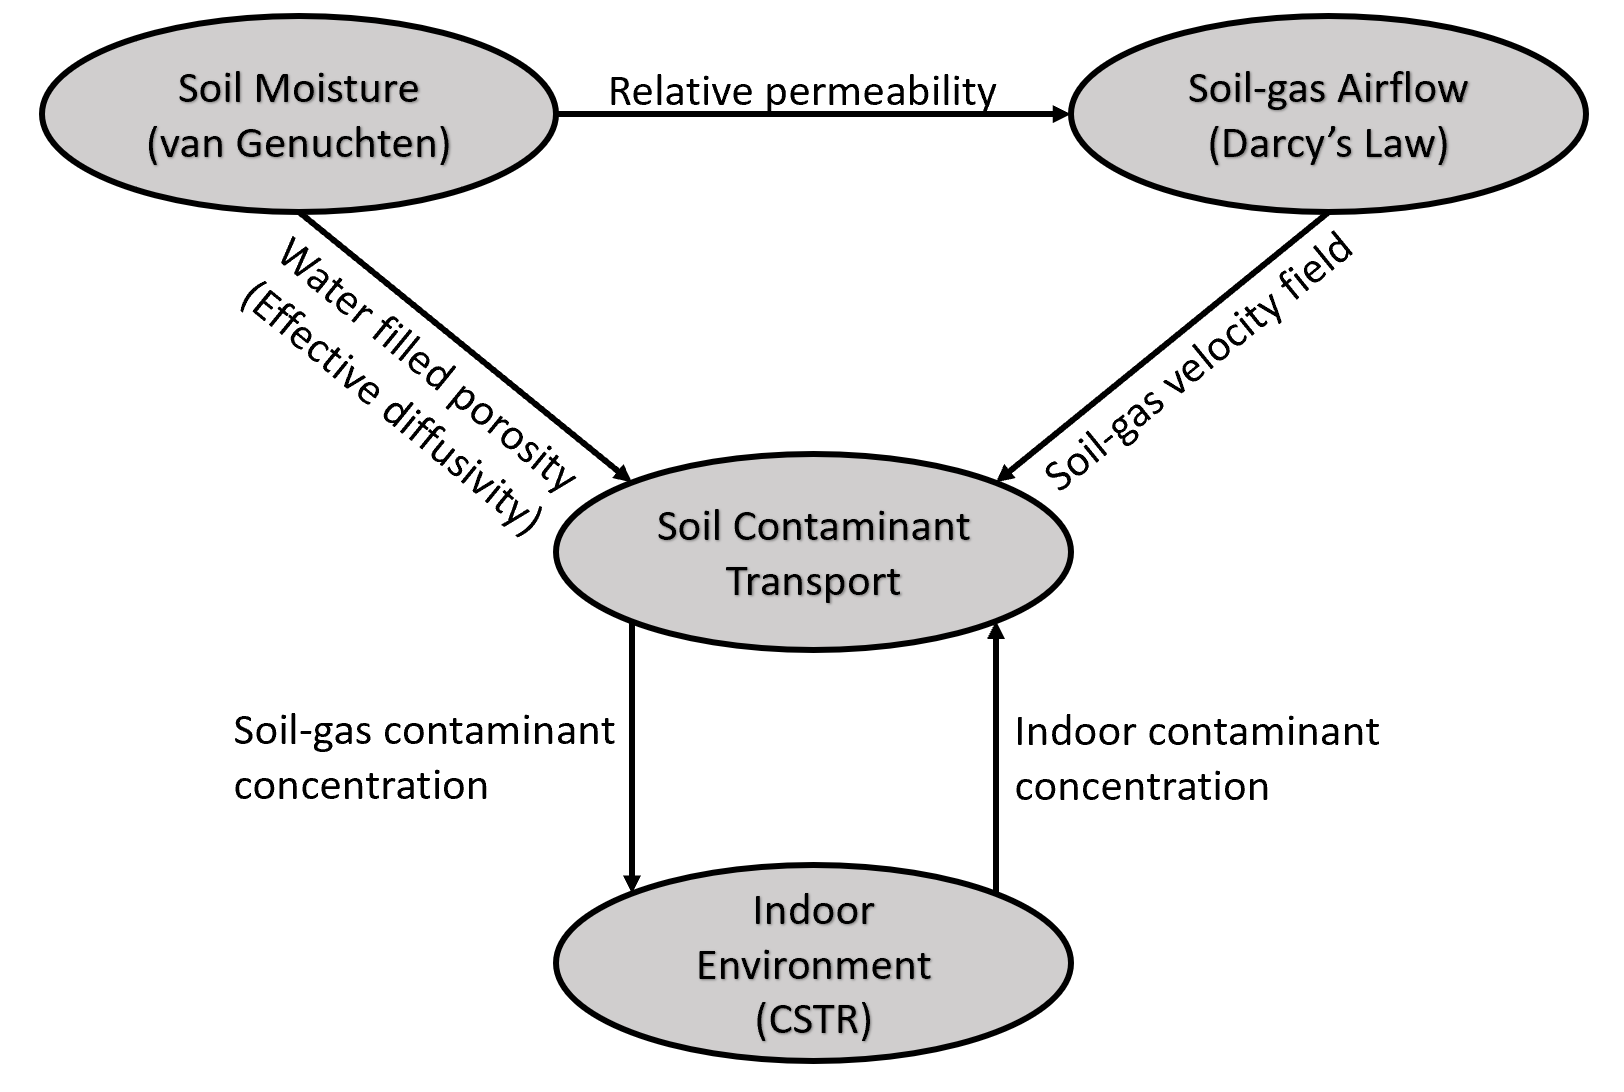
\includegraphics[width=\textwidth]{physics_interaction.png}
  \caption{Coupling between the physics used to model VI.}
  \label{fig:physics_overview}
\end{figure}

In this chapter, we will walk through the process of numerically modeling this VI scenario using the finite element method (FEM) and post-processing of the results.
A discussion regarding past and present VI models, their advantages and limitations, will follow.\par

\subsection{Finite Element Method}

% TODO Make it clear which sources I use here and say so early.
% TODO Make a figure showing the basis functions with nodal coefficients.

Many physical phenomena are described by partial differential equations (PDEs), but for anything but the simplest scenarios, these do not have an analytical closed-form solutions; therefore numerical methods are needed for finding an approximate solution.
This is achieved by discretizing the problem, i.e. transforming a continuous problem into a discrete one.
There are numerous ways to discretize a problem, and some of the more popular schemes are finite difference (FDM), finite volume (FVM), and finite element method (FEM).\par

In this work we use FEM, which is a popular numerical scheme that offers some distinct advantages over other schemes for modeling VI.
FEM subdivides the domain of the PDE problem into many smaller subdomains called elements.
These elements can take a wide variety of shapes, e.g. tetrahedra, prisms, or cuboids for three-dimensional problems and triangles or rectangles for two-dimensional problems.
The collection of elements that make up the domain or geometry is called a \textit{mesh}.
The fineness of the mesh is what largely determines the accuracy of the solution, but also increases the computational costs.\par

The size of each element can be highly nonuniform which allows FEM to discretize complicated geometries.
This is advantageous for modeling VI, where different parts of the geometry can have dramatically different resolution requirements; the \SI{1}{\centi\metre} foundation crack requires elements on the scale of \si{\milli\metre}, while in other parts of the geometry the resolution requirement is on the scale of \si{\metre}.
This ability to easily represent complicated geometries with elements of ununiform sizes helps maintain accuracy while saving computational resources.
Another benefit of using these elements is that it is easy to assign different constant values throughout the domain, and heterogenous materials can easily be represented.\par

The purpose of this work is not to provide a detailed description of the FEM, but for the interested reader \citeauthor{larson_finite_2010}\cite{larson_finite_2010} is a good resource.
However, it is important to know that FEM assumes that the approximated solution to a PDE can be written as a series of linear functions, called \textit{basis functions}.
\begin{equation}
  u \approx u_h = \sum^i u_i \psi_i
\end{equation}
here $u$ is the exact solution to the problem;
$u_h$ is the approximate solution;
$u_i$ is a \textit{nodal coefficient};
and $\psi$ is a \textit{basis function}.
These basis functions are usually some simple function, e.g. a hat function or some lower-order polynomial.\par

These basis functions are used to discretize the problem by rewriting a PDE into its \textit{weak form}, multiplying the equation with another set of functions called a \textit{test function}.
The test functions are the same type of function as the basis function, i.e. if the basis function is a hat function, so is the test function.
The result of this is an integral, where the integrands are the product of the basis function.
These integrals are numerically solved using some quadrature method, which gives a linear system of equations.
This system of equations is then solved to give all of the $u_i$ coefficients and thus the approximated solution $u_h$.\par

The point of this is that choice of basis function, i.e. hat function, first or third order polynomial, can influence the accuracy of the solution, and certain basis functions are more appropriate for certain PDEs.
Generally, higher order polynomials will give a more accurate solution, but at a computational cost, making it sometimes difficult to choose.
This adds another level of complexity of using FEM over some other numerical schemes, as the accuracy of the solution is not only influenced by the mesh but also somewhat by the choice of basis functions.
This highlights one of the drawbacks of FEM, i.e. that it is mathematically more challenging to implement and use than some other numerical schemes may be.\par

Fortunately, due to the attractiveness of the method, many commercial FEM packages have developed which increases usability significantly.
In this work we will use such a package - COMSOL Multiphysics, where subsequent sections will cover the steps required to implement our VI model in COMSOL.
(Of course, this could easily be translated into use in another software package.)\par

In order, we will cover:
\begin{enumerate}
  \item Creation of a model geometry.
  \item Defining physics/governing equations, boundary, and initial conditions.
  \item Discretize/mesh the geometry.
  \item Solver configuration.
  \item Post-process the results.
\end{enumerate}

\section{Geometry Generation}

Designing a good model geometry is critical as it can save significant computational resources.
When designing a geometry the FEM user should try to represent the model geometry as accurately as possible while:
\begin{enumerate}
  \item Avoid unnecessarily fine details; these may require an excessively fine mesh to resolve.
  \item Leverage symmetry to reduce the domain size over which solution must be effected, and thereby the mesh can be made finer in a smaller portion of the domain.
\end{enumerate}\par
Achieving these goals is not always straightforward, and success depends on the skill of the modeler and on the available tools.
Typically a model geometry is constructed in some computer assisted design (CAD) software, and the particular tools available in these packages vary.
While not absolutely necessary, the usa of a CAD package outside of the COMSOL solver might sometimes make development of the domain description easier.\par

\begin{figure}[htb!]
  \centering
  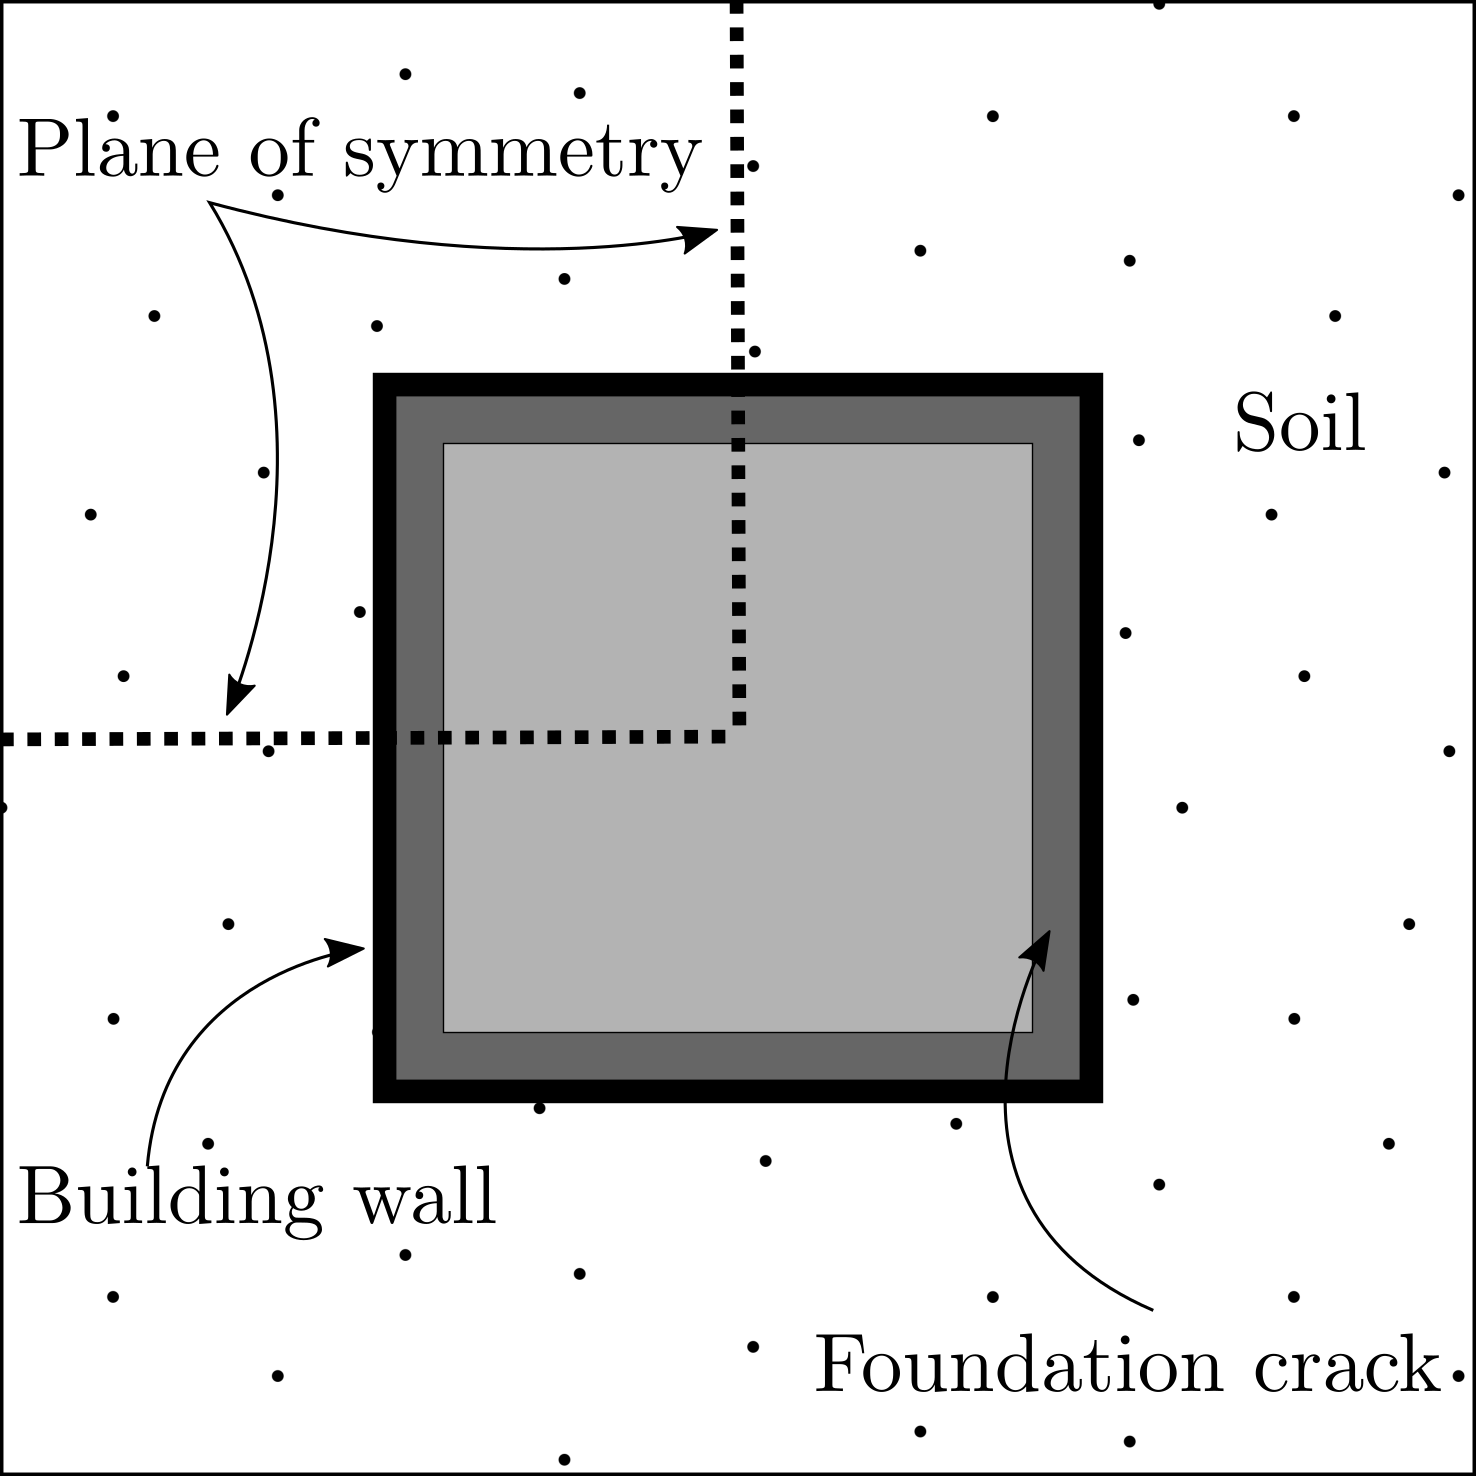
\includegraphics[width=0.75\textwidth]{symmetry.png}
  \caption{Birds-eye view of the VI scenario, showing the foundation and the breach, building wall, as well as the plane of symmetry that allows only a quarter of the total domain to be generated.}
  \label{fig:symmetry}
\end{figure}

COMSOL has a built-in geometry generation tool, which allows the construction of advanced geometries by performing various operations on simpler geometries, e.g. a cylinder and half sphere can be combined to make a rivet.
But as noted, it is also possible to import pre-generated geometries from other CAD software.
For present illustrative purposes, we will create our own geometry.\par

The interior of the house itself will not be explicitly modeled, instead we only consider the soil surrounding the house.
This is done for the simple reason that it is not important to model the interior of the house.
Once the contaminant is in the structure, the damage, so to speak, has been done.
We are interested in how fast the contaminant enters from the soil, which is what determines indoor contaminant concentration.
In addition, typical building interiors are simply too heterogenous to generalize in any meaningful way.
Trying to explicitly model the interior so as to offer insights into indoor concentration variations while at the same time modeling the necessary subsurface transport, would be prohibitively expensive.
Instead the interior is implicitly modeled as a CSTR and simply coupled with the explicit soil and foundation geometry via the foundation crack boundary.\par

One of the nice properties of the described VI scenario is that, due to symmetry, we only need to explicitly model a quarter of it (see Figure \ref{fig:symmetry}).
This reduces the number of required mesh points by 75\%, which is a huge computational saving.
To create the specified geometry, see the instructions for geometry generation in the appendix.

\begin{figure}[htb!]
  \centering
  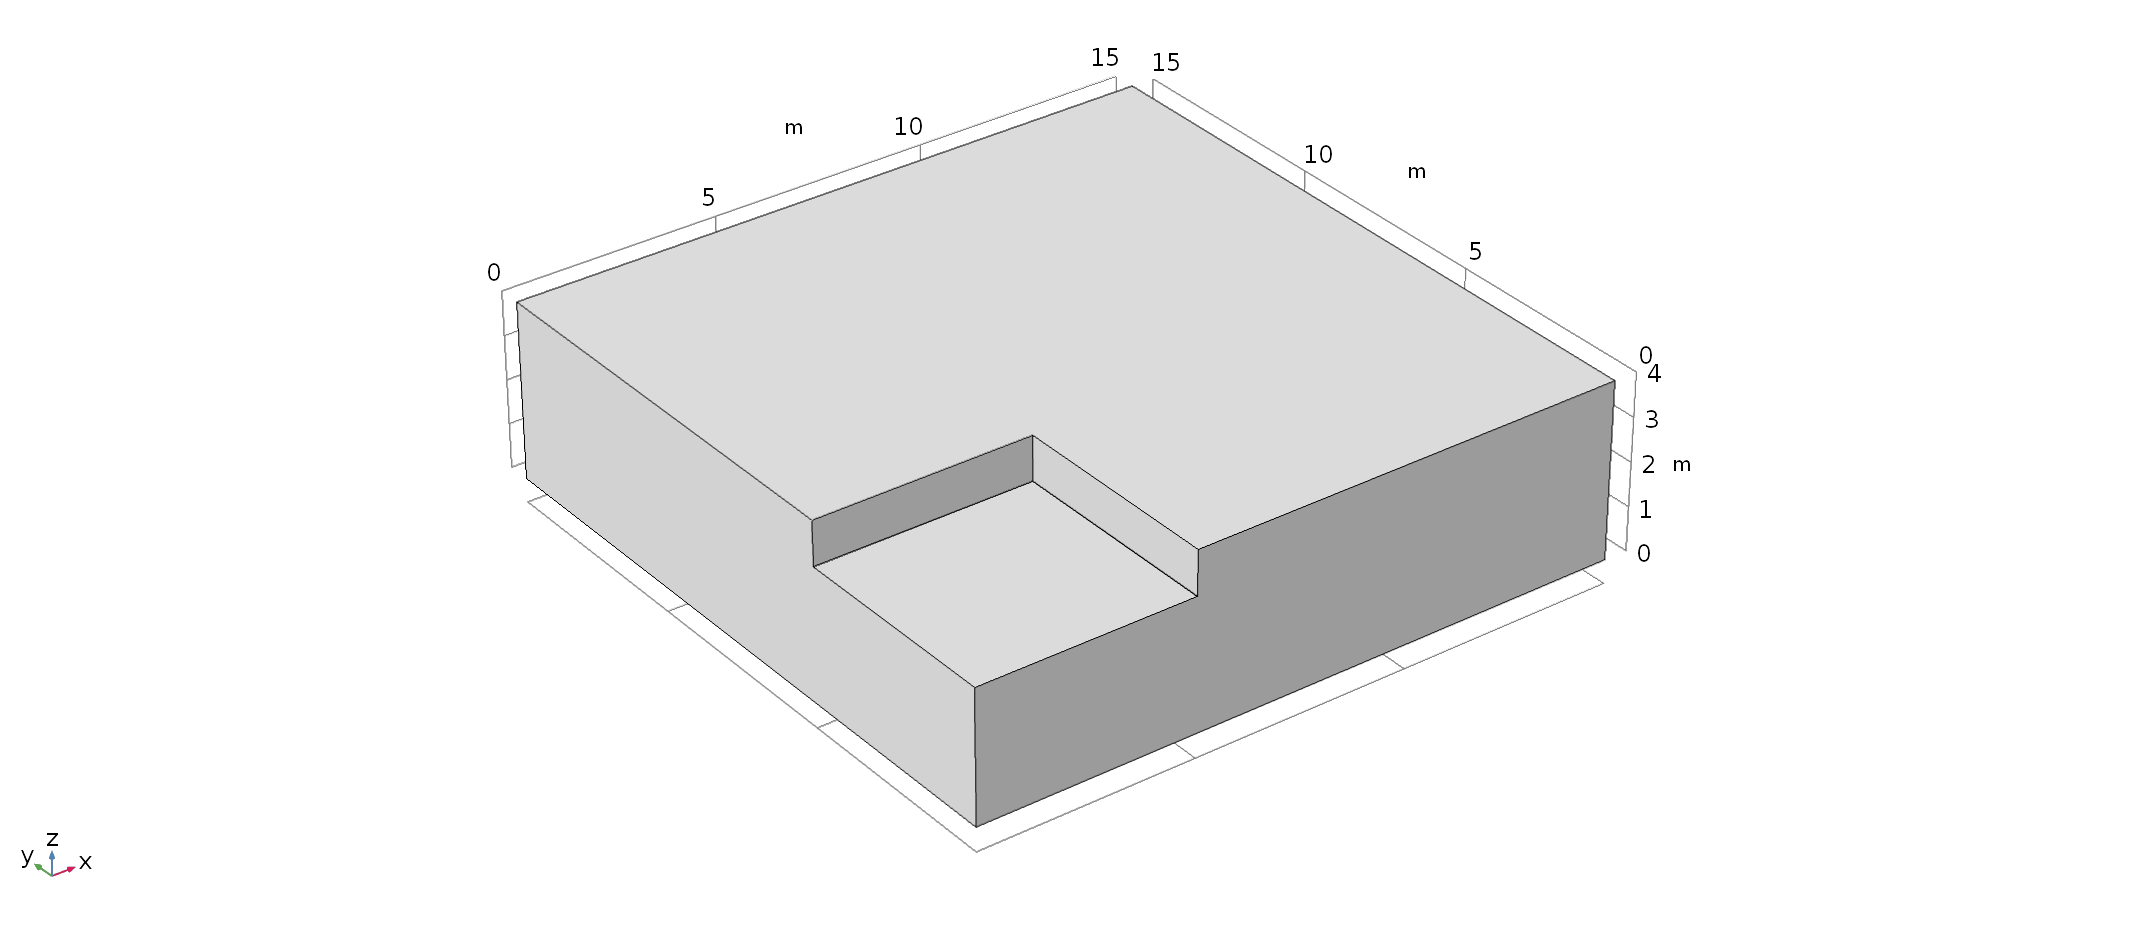
\includegraphics[width=\textwidth]{vi_model.png}
  \caption[VI model geometry in COMSOL]{The complete geometry of the VI scenario as implemented in COMSOL.}
  \label{fig:geometry}
\end{figure}

% Physics section and rest subsections?
\section{Vapor Intrusion Physics \& Govering Equations}

% A fantastic introduction/overview

% TODO: Add the figure that shows the relationships between the physics and all of the variables.

\subsection{The Indoor Environment}\label{sec:indoor}

The impacts on the indoor air space is perhaps the most important part of modeling VI, as the goal of these models ultimately is to predict indoor exposure given some external factors.
The indoor environment is, however, only modeled implicitly as a continuously stirred tank reactor (CSTR).
We assume that all contaminant entry into the house occurs via a foundation crack.
It has been shown in other modeling work that results are not overly sensitive to the nature and position of the actual foundation breach\cite{yao_simulating_2013}, so we do not need to be overly concerned about the nature of the crack - the key feature is the overall area that it presents for contaminant entry.
Once the contaminant enters the interior, it is instantly perfectly mixed, which is a key assumption of a CSTR.
Contaminant expulsion occurs via air exchange with the outdoor environment, and is regulated by \textit{air exchange rate} $A_e$, which dictates what fraction of the indoor air is exchanged with outdoor air over a given period of time.
For instance, a common air exchange rate for a house is $A_e = \SI{0.5}{\per\hour}$, i.e. half of the indoor air is exchanged every hour.
The impacts of air exchange rate will be explored in Chapter \ref{chp:preferential_pathways}.\par

It should be noted that in this simple VI model implementation, we assume that there are no indoor sources nor that any sorption of contaminant to/from any indoor materials occurs.
Thus, the reaction term that would ordinarily be part of a CSTR is dropped (but is reintroduced in Chapter \ref{chp:sorption}) and the temporal change in indoor contaminant concentration is thus given by \eqref{eq:cstr}.
\begin{equation}\label{eq:cstr}
  V_\mathrm{bldg}\frac{\partial c_\mathrm{in}}{\partial t} = n_\mathrm{ck} - V_\mathrm{bldg} A_e c_\mathrm{in}
\end{equation}
Here $c_\mathrm{in}$ [\si{\mol\per\metre\cubed}] is the indoor air contaminant concentration;
$n_\mathrm{ck}$ [\si{\mol\per\second}] is the contaminant entry (or exit) rate into the building via the foundation crack;
$A_e = \SI{0.5}{\per\hour}$ is the air exchange rate;
Finally, $V_\mathrm{bldg} = \SI{300}{\metre\cubed}$ is the volume of the house interior (or basement in this case).\par

A limitation of this approach is that we only consider one control volume or compartment, while in reality indoor contaminant concentrations can vary significantly between compartments, in particular between different floors.
There are VI models that use multiple compartments, which in essence are just coupled CSTRs\cite{murphy_multi-compartment_2011}.
Basements typically have higher indoor contaminant concentrations than other floors, so in this implementation we assume that our sole compartment is the house basement, which $V_\mathrm{bldg} = \SI{300}{\metre\cubed}$ reflects.\par

Solving \eqref{eq:cstr} requires us to determine the contaminant entry and air exchange rates.
Air exchange rates can vary quite significantly, and are a significant source of temporal variability in VI, a topic that will be further explored in Chapter \ref{chp:preferential_pathways}.
However, they typically vary around relatively well-known values as air exchange rates are regulated in building codes.
For residential buildings, it is typical that air exchange rate is around $A_e = \SI{0.5}{\per\hour}$ and thus for simplicity we will choose this value.\par

\paragraph{Contaminant entry into the building}

Contaminant entry rates are significantly more difficult to determine, as they depend on air velocity through the foundation breach and the concentration gradient across it.
The determination of these is the main point, and challenge in VI modeling.\par

\begin{figure}[htb!]
  \centering
  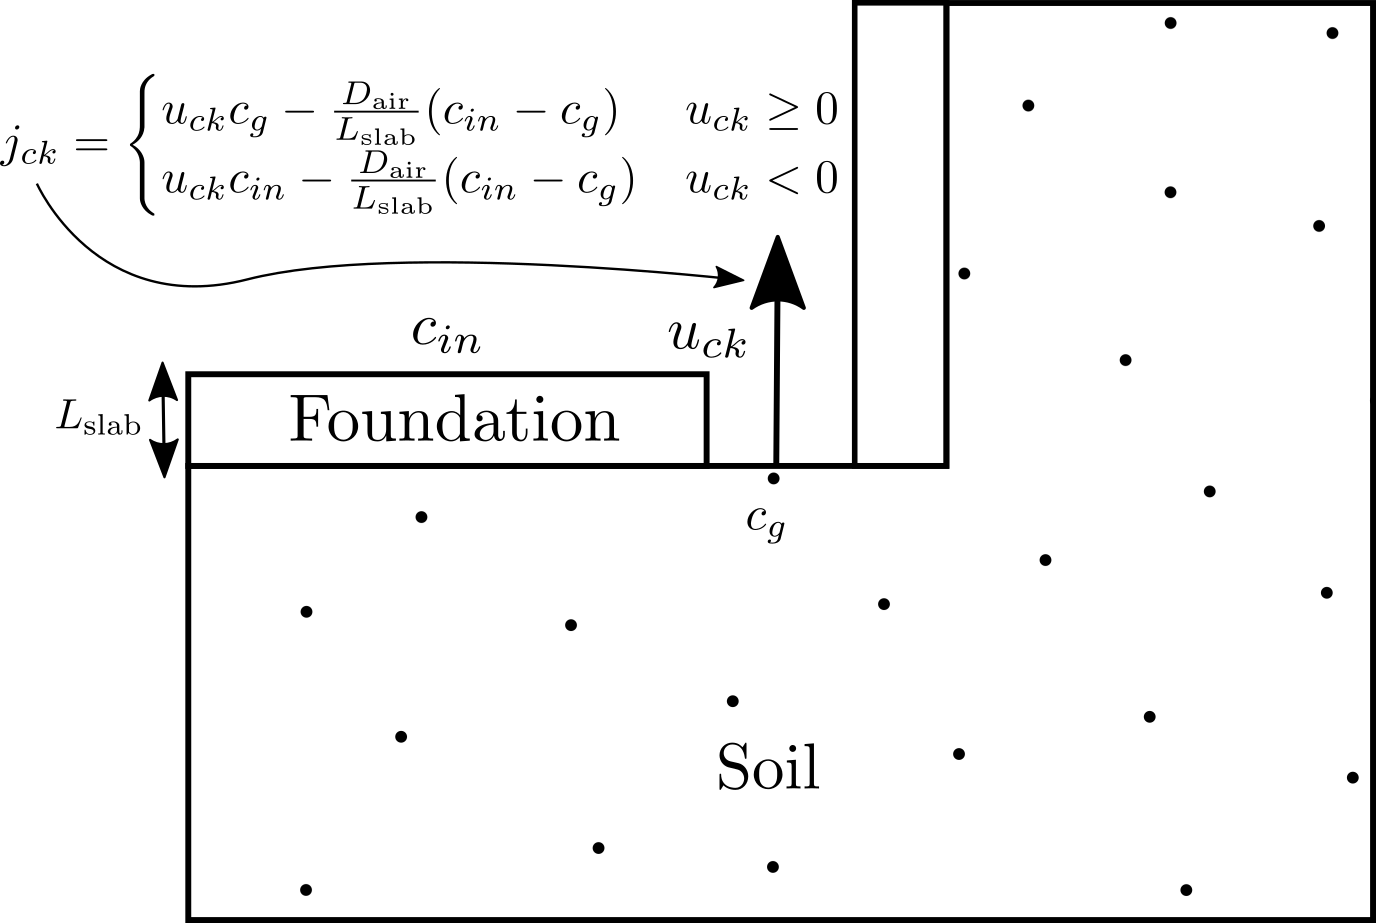
\includegraphics[width=0.6\textwidth]{crack_transport.png}
  \caption[Schematic of soil-gas contaminant entry into a building through a breach in the foundation.]{Soil-gas contaminant vapors are transported from the underlying soil into a building via a breach in the foundation. The scale is exaggerated, and in our modeled scenario the crack is only \SI{1}{\centi\metre} wide.}
  \label{fig:crack_transport}
\end{figure}

The contaminant entry $n_\mathrm{ck}$ is given by integrating the contaminant entry flux $j_\mathrm{ck}$ across the foundation crack boundary $A_\mathrm{ck}$.
\begin{equation}
  n_\mathrm{ck} = \int_{A_\mathrm{ck}} j_\mathrm{ck} dA
\end{equation}
The contaminant flux through the foundation crack is modeled as transport between two parallel plates and has an advective and a diffusive component.
\begin{equation}
  j_\mathrm{ck} = j_\mathrm{advection} + j_\mathrm{diffusion}
\end{equation}
Since contaminant concentration indoors is lower than it is in the soil or near foundation crack region a concentration gradient from the soil-gas to the indoor will exist.
The interior of the crack is not explicitly modeled, but assumed to only contain air and thus we assume the diffusion coefficient is the same as in air.
\begin{equation}
  j_\mathrm{diffusion} = - \frac{D_\mathrm{air}}{L_\mathrm{slab}} (c_{in} - c_g)
\end{equation}
here $D_\mathrm{air} = \SI{7.2e-6}{\metre\squared\per\second}$ is the diffusion coefficient of TCE in air as a sample contaminant of interest; other contaminant of common concern have comparable diffusivities.
$L_\mathrm{slab} = \SI{15}{\centi\metre}$ is a typical thickness of a foundation slab;
$c_{in}$ [\si{\mol\per\metre\cubed}] is the indoor contaminant concentration;
$c_g$ [\si{\mol\per\metre\cubed}] is the contaminant gas-phase concentration at the foundation crack boundary.\par

Advective transport through the slab can occur in both directions, i.e. contaminants can be carried from the soil into the house and from the house into the soil\cite{holton_creation_2018}.
The direction of this transport depend on the direction of the flow, with a positive sign indicating that airflow goes into the house.
\begin{equation}
  j_{advection} = \begin{cases}
    u_{ck} c_g & u_{ck} \geq 0 \\
    u_{ck} c_{in} & u_{ck} < 0
\end{cases}
\end{equation}
here $u_{ck}$ [\si{\metre\per\second}] is the airflow velocity through the foundation crack.

Thus the total contaminant transport through the foundation crack is given by \eqref{eq:contaminant_entry}.
\begin{equation}\label{eq:contaminant_entry}
  j_{ck} = \begin{cases}
    u_{ck} c_g - \frac{D_\mathrm{air}}{L_\mathrm{slab}} (c_{in} - c_g) & u_{ck} \geq 0 \\
    u_{ck} c_{in} - \frac{D_\mathrm{air}}{L_\mathrm{slab}} (c_{in} - c_g) & u_{ck} < 0
\end{cases}
\end{equation}
(See Figure \ref{fig:crack_transport}.)
Not only will \eqref{eq:contaminant_entry} be used to calculate the contaminant entry rate into house, but it is a necessary boundary condition for calculating the contaminant concentration in the soil.
However, as we see, \eqref{eq:contaminant_entry} is a function of both the soil-gas concentration at the foundation crack boundary $c_g$ and the indoor contaminant concentration $c{in}$, thus these two are coupled and need to be solved simultaneously.\par

\begin{comment}

To cover:

- Description of the physics that cause the variable soil moisture
- Modeling this
  - Correy & Brooks
  - van Genuchten

- Description of van Genuchten


\end{comment}
% TODO: How do I cite here when I basically use the same source for everything?

\subsection{Variable Soil Moisture Content}\label{sec:van_genuchten}

The portion of soil between groundwater and ground surface is variably saturated with water and is called the vadose zone.
Under environmental conditions, TCE and many other contaminants are miscible in water, and will be partitioned between its dissolved and vapor phases, which has profound effects on the total contaminant transport in the vadose zone.
The rates of diffusion in liquids and gases usually differ by orders of magnitudes. % TODO: Source
Likewise, advective transport in the two phases are vastly different, and as such it is important to account for the varying soil moisture content.\par % TODO: Source

Water filling of soil pores from groundwater is driven by a negative pressure gradient induced by surface tension, called capillary potential and is here represented by $\psi$.
This capillary potential is a function of the soil moisture content, and becomes increasingly negative as the water content decreases, and is zero when the soil matrix is saturated with water.
The capillary potential varies with the hydraulic properties of specific soil types.\par

In addition to the capillary potential, soil moisture content is driven by a gravitational potential, e.g. groundwater flow in soil.
The total soil moisture potential $\phi$, is the sum of the capillary and gravitational potentials, here expressed as a pressure head.
\begin{equation}
  \phi = \frac{\psi(\theta_w)}{\rho g} + h_\mathrm{g} = h + h_\mathrm{g}
\end{equation}
where $\phi$ [\si{\metre}] is the total soil moisture potential (as a pressure head);
$\psi$ [\si{\pascal}] is the capillary potential;
$h$ [\si{\metre}] is the capillary potential as a pressure head above the groundwater/soil interface;
$\theta_w$ is the volumetric moisture content by volume soil, i.e. dimensionless;
$\rho$ [\si{\kilo\gram\per\metre\cubed}] is the density of water;
$g$ [\si{\metre\per\second\squared}] is the acceleration due to gravity;
and $h_\mathrm{g}$ [\si{\metre}] is the gravitational potential above a reference plane.\par

In the VI scenario considered here, we assume that there is no gravitational potential, and thus that the soil moisture content is at steady-state.
This simplifies the determination of the soil moisture content, which now is entirely determined by the capillary potential $\psi$, or $h$ in our case.\par

There are two common methods for modeling the capillary potential, one developed by \citeauthor{brooks_properties_1966}\cite{brooks_properties_1966} in 1966, and another by \citeauthor{van_genuchten_closed-form_1980}\cite{van_genuchten_closed-form_1980} in 1980.
Both of these are semi-empirical approaches and relies on experimentally determined parameters for a specific soil type to be used.
In this work, we only use van Genuchten's method, simply because parameters for a wide variety of soils have been made available by the EPA and may be seen in Table \ref{tbl:soils}.\par

If the assumption that there is no gravitational potential cannot be made, then the full soil moisture potential $\phi$ needs to be determined.
This is achieved by solving Richard's equation.\par % TODO: Write about Richard's equation and reference it?

\subsubsection{van Genuchten's Soil-Water Retention Model}

% TODO: Make sure the sign or absolute |h| should be here or not.
The relationship between capillary pressure and moisture content is called \textit{soil moisture retention}, and is what van Genuchten's method models.
Specifically, his method models the water saturation of the soil and is given by \eqref{eq:van_genuchten_saturation}.
\begin{equation}\label{eq:van_genuchten_saturation}
  \mathrm{Se} =
    \begin{cases}
      \frac{1}{(1 + (\alpha |h|)^n)^m} & h < 0 \\
    1 & h \geq 0
    \end{cases}
\end{equation}
here $\mathrm{Se}$ is the saturation, which ranges from 0 to 1, where 1 is fully saturated with water;
$\alpha$, $m$, and $n=\frac{1}{1-m}$ are the empirically determined van Genuchten parameters and can be seen in Table \ref{tbl:soils};
and $h$ [\si{\metre}] is the capillary pressure head, which in this case is the elevation above the groundwater/soil interface.\par

It is important to note that $\mathrm{Se} = 0$ does not mean that there is no moisture in the soil, but soils retain a small amount of water in the matrix - residual moisture content (which again is soil specific).
Thus, the soil moisture content is given by \eqref{eq:van_genuchten_soil_moisture}
\begin{equation}\label{eq:van_genuchten_soil_moisture}
  \theta_w =
    \begin{cases}
      \theta_r + \mathrm{Se}(\theta_t - \theta_r) & h < 0 \\
      \theta_t & h \geq 0
    \end{cases}
\end{equation}
where $\theta_w$ is the volumetric soil moisture content;
$\theta_t$ is the soil porosity;
and $\theta_r$ is the residual moisture content.\par

By extension, the soil gas or air content is given by
\begin{equation}\label{eq:gas_porosity}
  \theta_g = \theta_t - \theta_w
\end{equation}
An example of the soil saturation and moisture content as a function of pressure head is shown in Figure \ref{fig:retention_curve}.
Note the steep decline in moisture content near the groundwater interface - that is the capillary zone and we will see that it presents a significant barrier to contaminant transport from the groundwater in section \ref{sec:transport}.\par

\begin{figure}
  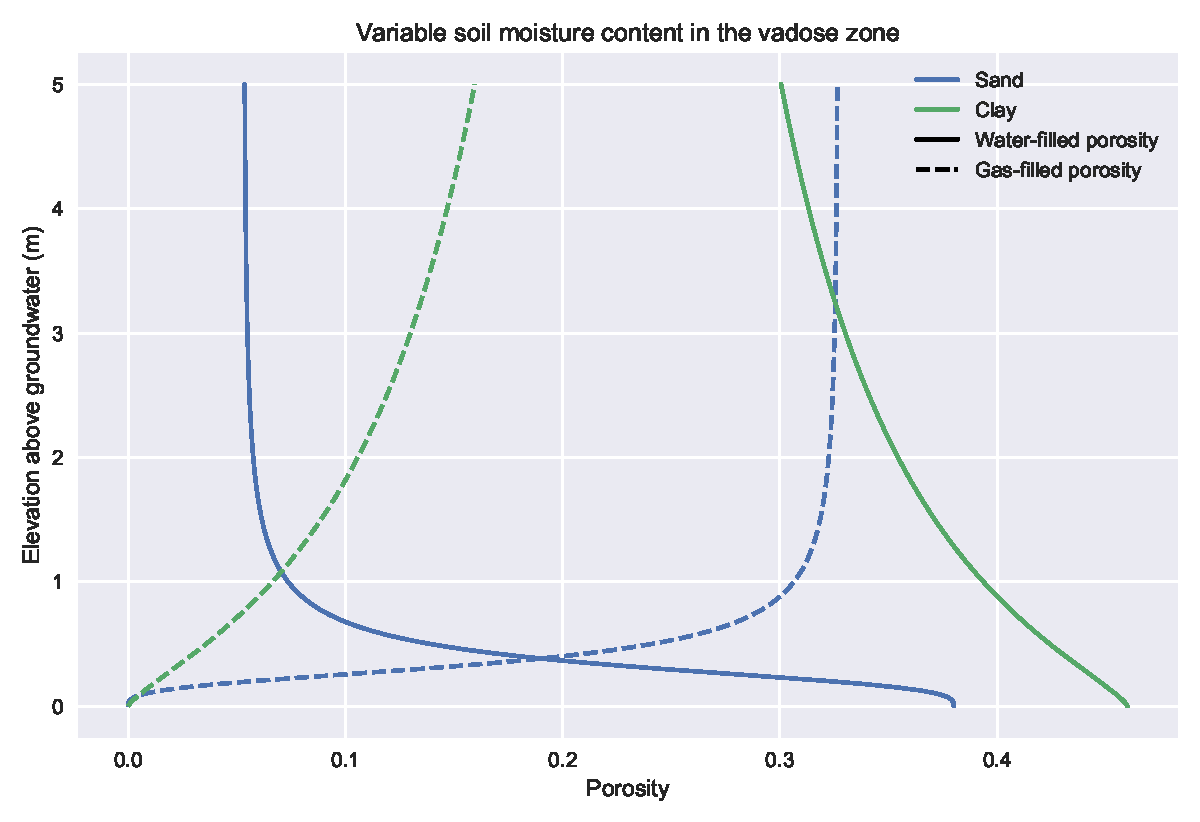
\includegraphics[width=\textwidth]{van_genuchten.pdf}
  \caption{Example of a soil moisture retention curve as a function of pressure head above the groundwater/soil interface.}
  \label{fig:retention_curve}
\end{figure}

The presence of water in the soil matrix has profound implications for transport as the pore space may be restricted to only one phase.
For instance, in the capillary zone, the only possible bulk transport in the water phase, while gas phase transport is impossible.
The opposite is true near the ground surface, where most of the pore space consists of air.\par

Soil already limits transport for a single phase due to its permeability, i.e. it is harder to pump water through a soil columns than a pipe of the same size.
This extra phase-specific transport inhibition is modeled as a \textit{relative permability} and is given by \eqref{eq:van_genuchten_relative_permeability}.
\begin{equation}\label{eq:van_genuchten_relative_permeability}
  k_r =
    \begin{cases}
      \mathrm{Se}^l \big[ 1 - \big( 1 - \mathrm{Se}^\frac{1}{m} \big) \big]^2 & h < 0 \\
      0 & h \geq 0
    \end{cases}
\end{equation}
here $k_r$ is the relative permeability for water; % TODO: Make sure that is right
and $l = 0.5$ is another van Genuchten parameter.\par % TODO: How do I motivate this?

The relative permeability varies from 0 to 1, where 0 indicates that the soil matrix is completely impermeable to the fluid, while a value of 1 means that there is no additional permeability cost.
Since $k_r$ here is relative to water, the gas phase relative permeability is given by $1 - k_r$.
Figure \ref{fig:relative_permeability} shows how the relative gas and water permeability varies in the vadose zone.\par

\begin{figure}
  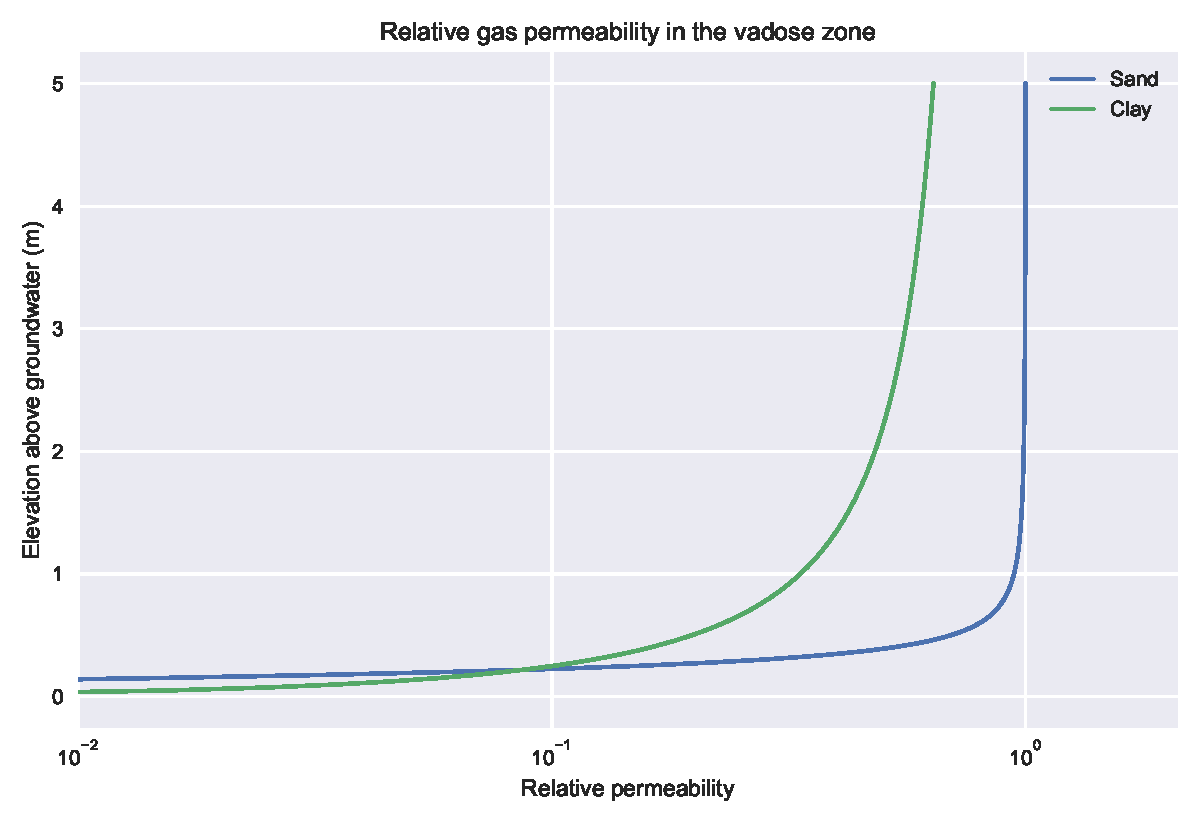
\includegraphics[width=\textwidth]{relative_permeability.pdf}
  \caption{Relative gas and water permeability in the vadose zone or above the groundwater interface.}
  \label{fig:relative_permeability}
\end{figure}

\begin{comment}
% TODO: Move this to where Richard's equation is described.
\begin{equation}\label{eq:van_genuchten_moisture_capacity}
  C_m =
    \begin{cases}
      \frac{\alpha m}{1-m}(\theta_s - \theta_r)\mathrm{Se}^{\frac{1}{m}}\big( 1 - \mathrm{Se}^{\frac{1}{m}} \big)^m & h < 0 \\
    0 & h \geq 0
    \end{cases} \\
\end{equation}
\end{comment}

\subsection{Airflow In The Vadose Zone}\label{sec:darcys_law}

In our VI scenario, the depressurized house induces an advective airflow from the ground surface, through the vadose zone, and into the house via a foundation crack, this flow carries contaminant vapors with it.
This airflow is modeled using a modified version of Darcy's Law.
The modification is made to account for the variable moisture content in the vadose zone, which is discussed in section \ref{sec:van_genuchten}.\par

Darcy's Law describes the flow of a fluid through a porous medium.
This flow is typically driven by a pressure gradient, and its magnitude depends on the permeability of the porous medium and the fluid's viscosity.
\begin{equation}\label{eq:darcys_law_saturated}
  \vec{u} = -\frac{\kappa}{\mu} \nabla p
\end{equation}
here $\vec{u}$ [\si{\m\per\second}] is the airflow velocity vector;
$\kappa$ [\si{\metre\squared}] is the permeability of the porous medium;
$\mu$ [\si{\pascal\second}] is the dynamic viscosity of the fluid;
and $\nabla p$ [\si{\pascal\per\metre}] is the pressure gradient.\par

This \eqref{eq:darcys_law_saturated} formulation of Darcy's Law assumes that the porous medium is saturated with the transporting fluid,\footnote{Darcy's Law also assumes that the flow is in the laminar regime, i.e. the Reynolds number $\mathrm{Re} < 1$.
Due to the small pressure gradients in most VI scenarios, this assumption is rarely unfulfilled, but if it is, then Brinkman's equation should be used instead.}
hence the need to modify this expression when there are two fluid phases present.
While porosity is not directly part of \eqref{eq:darcys_law_saturated}, it is an intrinsic property that determines the permeability $\kappa$ of the porous medium; the degree of saturation in pores determines the air permeability.
This variation in permeability is modeled using the relative permeability expression from van Genuchten's equation \eqref{eq:van_genuchten_relative_permeability}.
The effective soil permeability is the product of the saturated soil permeability and its relative permeability giving our modified Darcy's Law \eqref{eq:darcys_law_unsaturated}.
\begin{equation}\label{eq:darcys_law_unsaturated}
  \vec{u} = -\frac{k_r\kappa}{\mu} \nabla p
\end{equation}
Recall that by definition $k_r$ is the relative permeability of the soil to \textit{air}, and thus $k_r\kappa$ form an effective permeability.\par

To calculate the soil-gas velocity field in the vadose zone, we need a continuity equation, which for fluid flow is \eqref{eq:fluid_continuity}.
\begin{equation}\label{eq:fluid_continuity}
  \frac{\partial \rho}{\partial t} + \nabla \cdot (\rho \vec{u}) = 0
\end{equation}
Inserting our modified Darcy's Law for the velocity gives \eqref{eq:vapor_transport}.
\begin{equation}\label{eq:vapor_transport}
  \frac{\partial}{\partial t} (\rho \theta_g) + \nabla \cdot \rho \Big( -\frac{(1-k_r) \kappa}{\mu} \nabla p \Big) = 0
\end{equation}
where $\theta_g$ is the gas-filled porosity of the soil from \eqref{eq:gas_porosity};
$\rho = \SI{1.225}{\kilogram\per\metre\cubed}$ is the density of air;
and $\mu = \SI{18.5e-6}{\pascal\second}$ is the dynamic viscosity of air.
Contaminant vapor concentrations are typically very low in VI scenarios, and therefore we assume that the contaminant does not affect the transport properties of air.\par

In order to solve \eqref{eq:vapor_transport} we need to define some boundary conditions.
In our VI scenario, air is pulled from the atmosphere through the ground surface and into the building via the foundation crack.
To model this only three boundary conditions are required.
We also need to choose a basis function, and we use the COMSOL recommended "hat" here, which will be used to determine the pressure $p$ throughout the modeled domain.\par

\paragraph{Boundary Conditions}

The first boundary condition defines a pressure gauge, i.e. a reference point for where the pressure is zero, and is where air will be pulled from.
This is applied to the ground surface boundary.
The second is that we apply the indoor/outdoor pressure difference (-5 Pa) to the foundation crack boundary, assuming that the indoor air pressure exists at the crack entrance at the soil interface.
The third type of boundary condition is applied to all remaining boundaries and is a no flow boundary condition, indicating that no flow passes through these boundaries.
This also applies to the symmetry planes present recalling that we are solving over only a quarter domain.
\begin{align}
  &\text{Ground surface} &p = \SI{0}{\pascal} \\
  &\text{Foundation crack} &p = p_\mathrm{in/out} =\SI{-5}{\pascal} \\
  &\text{Remaining} &-\vec{n}\cdot\rho\vec{u} = 0
\end{align}
where $\vec{n}$ is the boundary normal vector.\par

\paragraph{Initial Conditions}

For steady-state problems, initial conditions are not needed.
Transient simulations however, require initial conditions and these are typically assumed to be given by some steady-state solution that exists before a transient disruption.\par

\subsection{Mass Transport In The Vadose Zone}\label{sec:transport}

To begin deriving a governing equation for contaminant transport in our VI scenario, we consider the continuity equation which states that the change of concentration in some volume of space depends on the advective and diffusive fluxes in and out of the system, as well as any generation or consumption inside the system.
\begin{equation}
  \frac{\partial c}{\partial t} + \nabla \cdot(j_\mathrm{adv} + j_\mathrm{diff}) - G = 0
\end{equation}
here $c$ [\si{\mol\per\metre\cubed}] is the concentration of the chemical species;
$t$ [\si{\second}] is time;
$j_\mathrm{adv}$ and $j_\mathrm{diff}$ [\si{\mol\per\second\per\metre\squared}] are the advective and diffusive fluxes respectively;
and $G$ [\si{\mol\per\second}] is the generation or consumption of the chemical species.\par

In our model we will assume that $G = 0$ as the groundwater is the sole contaminant source, i.e. there are no other sources of TCE in the soil, and TCE also does not readily degrade in soils\footnote{
Although, it is possible to introduce certain bacteria to bioremediate TCE in soils, but this typically requires specific conditions, which generally are not naturally met. Under these specific conditions TCE may be biodegraded by some bacteria\cite{fan_biodegradation_1993,little_trichloroethylene_1988}
}.
However, this term should be retained and an appropriate expression developed if one wants to model:
\begin{itemize}
  \item Biodegradation of some compound in the soil.
  \item Radon intrusion (remember radon gas is generated throughout soils and rocks).
  \item A soil or subsurface source, e.g. a leaky tank or evaporation from a liquid contaminant spill.
\end{itemize}\par

The advective flux is given by
\begin{equation}
  j_\mathrm{adv} = \vec{u} c
\end{equation}
where $\vec{u}$ [\si{\metre\per\second}] is a velocity vector.
The diffusive flux is given by Fick's Law
\begin{equation}
  j_\mathrm{diff} = -D \nabla c
\end{equation}
where $D$ [\si{\metre\squared\per\second}] is the diffusion coefficient of the contaminant in the soil air;
and $\nabla c$ [\si{\mol\per\metre\cubed\per\metre}] is a concentration gradient.
Thus we get the advection-diffusion equation which generally governs transport of a chemical species
\begin{equation}\label{eq:adv_diff}
  \frac{\partial c}{\partial t} + \nabla \cdot(\vec{u} c + -D \nabla c) = 0
\end{equation}
However, this simple gas phase transport equation will not accurately represent contaminant transport in the vadose zone if:
\begin{itemize}
  \item Contaminant transport occurs inside a variably saturated porous matrix which significantly affect transport properties.
  \item The contaminant concentration in the vadose zone is distributed between three phases - gas, water, and solid (via sorption).
\end{itemize}\par

The total contaminant concentration in the soil is given by the sum of the gas, water, and solid phase concentrations at any given point in the soil.
\begin{equation}
  c_T = \theta_w c_w + \theta_g c_g + c_s \rho_b
\end{equation}
Here $\theta_g$ and $\theta_w$ are the gas-filled and water-filled porosities respectively;
$c_T$ [\si{\mol\per\metre\cubed}] is the total soil contaminant concentration;
$c_w$ and $c_g$ [\si{\mol\per\metre\cubed}] are the contaminant concentrations in water and gas respectively;
$c_s$ [\si{\mol\per\kilogram}] is the solid phase or sorbed concentration per mass of soil;
and $\rho_b = (1-\theta_t) \rho$ [\si{\kilogram\per\metre\cubed}] is the bulk density of the soil, which can be calculated from the soil porosity $\theta_t$ and solid phase density of the soil $\rho$ [\si{\kilogram\per\metre\cubed}].\par

The attentive reader will now notice that \eqref{eq:adv_diff} depends on three variables instead of one.
However, remember that we're concerned with low contaminant concentrations, we can relate the gas and liquid phase concentrations via Henry's Law \eqref{eq:henrys_law}
\begin{equation}\label{eq:henrys_law}
  c_g = K_H c_w
\end{equation}
where, for example $K_H = 0.402$ is the dimensionless Henry's Law constant for TCE at \SI{20}{\degreeCelsius}\cite{heron_henrys_1998}.
We also assume that there are no temperature gradients throughout the vadose zone.\par

The solid phase concentration can be related to the others via a linear sorption isotherm.
Here either the gas-solid or water-solid sorption interaction can be chosen; the former is used in Chapter \ref{chp:sorption} where we will explore the effects of gas-solid sorption.
\begin{equation}
  c_s = \begin{cases}
    K_p c_w & \text{Water-solid sorption} \\
    K_p c_g = K_p K_H c_w & \text{Gas-solid sorption}
\end{cases}
\end{equation}
here $K_p$ [\si{\metre\cubed\per\kilogram}] is a sorption partitioning coefficient.\par

Another approach is to simply ignore the role of sorption completely, i.e. $K_p = 0$, which has historically been done in VI modeling and is done in the following parts of this example too.
The reason for this is two-fold.
\begin{enumerate}
  \item Relevant soil sorption data have not been readily available.
  \item At steady-state, sorption doesn't affect the solution; the fact that there is TCE sorbed to soil particles does not influence the vapor transport at steady state, since equilibrium is assumed to have been established prior to the steady-state analysis. This has been a common assumptions in most VI modeling studies, which have mostly focused on steady-state.
\end{enumerate}
Regardless, we will continue carrying the sorption $K_p$ term, because this will become relevant in Chapter \ref{chp:sorption} where experimentally derived relevant sorption data are available, and in which the role of this sorption process is considered in the context of transient models.\par

Using Henry's Law and the linear sorption assumptions we can relate the total contaminant concentration at any point in the soil matrix to the water-phase contaminant concentration at that point, from which the air phase and solid phase concentrations may be immediately calculated.
The focus on water concentration is arbitrary, but commonly used.
\begin{equation}
  c_T = (\theta_w + \theta_g K_H + K_H K_p \rho_b) c_w
\end{equation}
The terms in front of $c_w$ are collected as $R = (\theta_w + \theta_g K_H + K_H K_p \rho_b)$.
This term is called the \textit{retardation factor} and reflects the potentially increased contaminant residence time in the matrix due to transferring between the phases.
Again, this only becomes an important factor in transient transport simulations.\par

In the vadose zone, advective transport can occur in both the water and gas phases inside the soil pores.
\begin{equation}
  j_\mathrm{adv} = \vec{u}_{w,pore} c_w \theta_w + \vec{u}_{g,pore} c_g \theta_g
\end{equation}
here $\vec{u}_{w,pore}$ and $\vec{u}_{g,pore}$ [\si{\metre\per\second}] are the water and gas phase \textit{pore} velocities vectors respectively.
However, from mass conservation, we know that the product of the pore velocity and porosity gives the superficial velocity of a fluid in porous media, i.e. the Darcy's Law velocities.
This together with Henry's Law gives
\begin{equation}
  j_\mathrm{adv} = (\vec{u}_w + \vec{u}_g K_H ) c_w
\end{equation}
and here $\vec{u}_w$ and $\vec{u}_g$ [\si{\metre\per\second}] are the Darcy or superficial velocity vectors.\par

In section \ref{sec:van_genuchten} we assumed that soil-water is stationary, i.e. $\vec{u}_w = 0$ giving
\begin{equation}
  j_\mathrm{adv} = \vec{u}_g K_H c_w
\end{equation}
where $\vec{u}_g$ is the solution obtained from solving Darcy's Law in section \ref{sec:darcys_law}.\par

To model a scenario where there is a gravitational water potential resulting in groundwater flow, one would have to solve two-phase Darcy's Law to get both $\vec{u}_g$ and $\vec{u}_w$.
This significantly complicates the mass transport aspect as well, and as such is beyond the scope of this work.
This rarely contributes much to understanding VI and the rates of groundwater movement are typically too slow to be of much consequence.\par

The diffusive transport expression likewise needs to be adjusted for multiphase systems, and the total diffusive flux through the pore matrix is given by
\begin{equation}
  j_\mathrm{diff} = -(D_w \theta_w \tau_w \nabla c_w + D_g \theta_g \tau_g \nabla c_g)
\end{equation}
here $D_w = \SI{1.02e-9}{\metre\squared\per\second}$ and $D_g = \SI{6.87e-6}{\metre\squared\per\second}$ are the contaminant diffusion coefficients of TCE in pure water and air respectively;
and $\tau_w$ and $\tau_g$ are the water and gas tortuosity terms, reflecting the fact that in a granular bed, the flow does not occur in a straight line direction.\par

Due to the irregular shapes of pores, diffusion of a chemical species will inevitably often occur along a tortuous path, which the tortuosity terms attempt to capture.
As tortuosity depends on the structure of the porous matrix, it is difficult to accurately portray, but a popular approach is to use the Millington and Quirks model\cite{millington_permeability_1961}.
\begin{equation}\label{eq:millington-quirk}
  \tau_w = \frac{\theta_w^{\frac{7}{3}}}{\theta_t^2}, \; \tau_g = \frac{\theta_g^{\frac{7}{3}}}{\theta_t^2}
\end{equation}
here $\theta_t$ is the total or saturated porosity of the soil matrix.
Another popular approach is Bruggeman's model.\par

Combining \eqref{eq:millington-quirk} and \eqref{eq:henrys_law} in our diffusion flux expression gives
\begin{equation}
  j_\mathrm{diff} = -\Big(D_w \frac{\theta_w^{\frac{10}{3}}}{\theta_t^2} + D_g \frac{\theta_g^{\frac{10}{3}}}{\theta_t^2} K_H\Big) \nabla c_w
\end{equation}
the terms in front of $\nabla c_w$ can be collected as an effective diffusion coefficient $D_\mathrm{eff}$ [\si{\metre\squared\per\second}], which with our isothermal vadose zone assumption only depends on the soil moisture content.
Thus we get the final diffusive flux expression
\begin{equation}
  j_\mathrm{diff} = - D_\mathrm{eff}\nabla c_w
\end{equation}
Figure \ref{fig:D_eff} shows how the effective diffusivity varies from being close to that of the pure water diffusivity near the capillary zone, and increases to something closer to gas-phase diffusivity as the soil moisture decreases.\par

\begin{figure}[htb!]
  \centering
  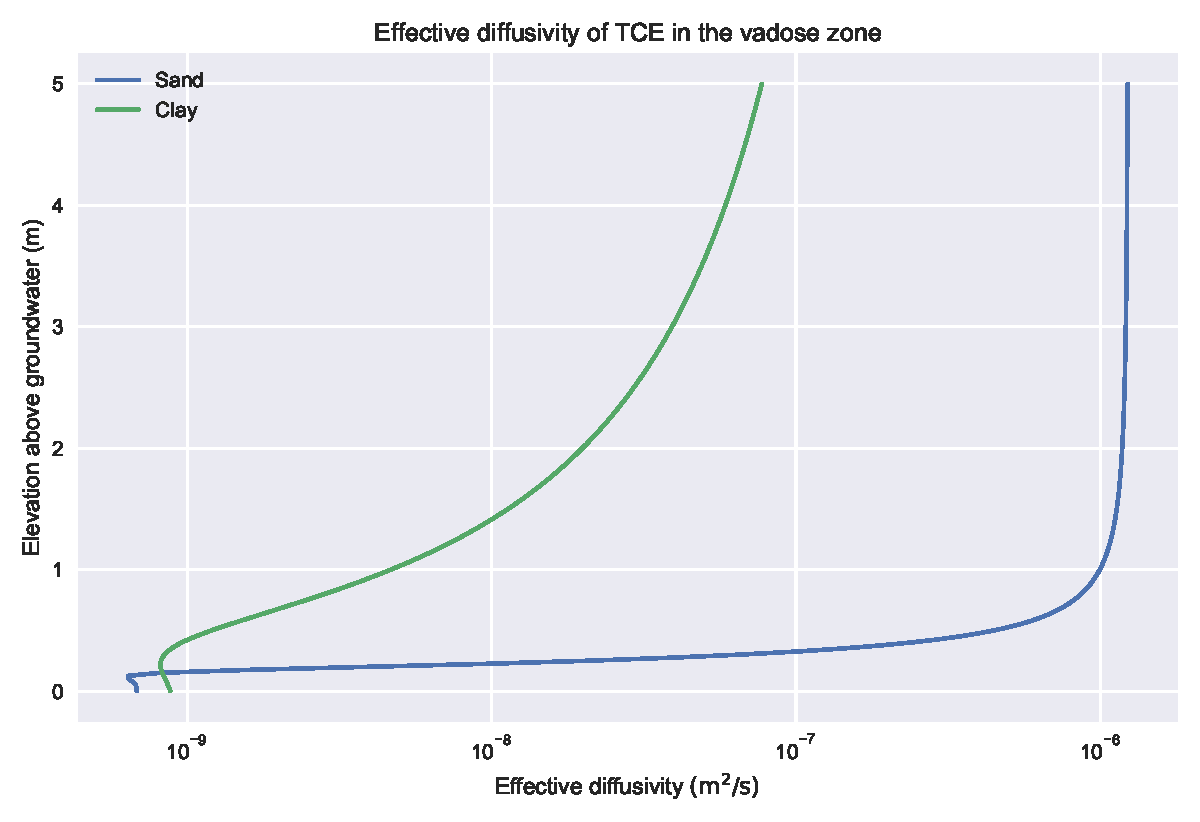
\includegraphics[width=0.75\textwidth]{effective_diffusivity.pdf}
  \caption[Effective diffusivity of TCE in the vadose zone.]{Effective diffusivity of TCE in the vadose zone using the Millington-Quirk model. Soil water and gas filled porosites are calculated using van Genuchten's equations.}
  \label{fig:D_eff}
\end{figure}

Putting all this together finally gives us the governing equation for contaminant transport in the vadose zone for our modeled VI scenario.
\begin{equation}\label{eq:mass_transport}
  R \frac{\partial c_w}{\partial t} = \nabla \cdot (D_\mathrm{eff} \nabla c_w) - K_H \vec{u}_g \cdot \nabla c_w
\end{equation}
To solve this we need to define some boundary and initial conditions.
We also need to choose a basis function which is used to determine the contaminant concentration throughout the domain, and we use the COMSOL recommended second order polynomial here.\par

\paragraph{Boundary Conditions}

In this VI scenario, the sole contaminant source is assumed to be the homogenously contaminated groundwater, which we assume to have a fixed concentration.
The atmosphere acts as a contaminant sink and thus this is simply a zero concentration boundary condition.
Contaminants leave the soil domain and enter the building through a combination of advective and diffusive gas phase transport.
The boundary condition applied to all other boundaries is a no-flow boundary.
\begin{align}
  &\text{Atmosphere} & c_w = \SI{0}{\mol\per\metre\cubed} \\
  &\text{Groundwater} & c_w = c_{gw} = \SI{50}{\micro\mol\per\metre\cubed} \\
  &\text{Foundation crack} & -\vec{n} \cdot \vec{N} = -j_{ck} \; \si{\mol\per\metre\squared\per\second}\\
  &\text{All other} & -\vec{n} \cdot \vec{N} = \SI{0}{\mol\per\metre\squared\per\second}
\end{align}
$\vec{n} \cdot \vec{N}$ is the dot product between the boundary normal vector and the contaminant flux;
$j_ck$ [\si{\mol\per\metre\squared\per\second}] is the contaminant flux into the building from section \ref{sec:indoor}.\par

\paragraph{Initial Conditions}

For steady-state problems, the initial conditions do not enter.
Transient simulations however, require initial conditions and these are assumed to be given by the steady-state solution.\par

\section{Meshing}\label{sec:meshing}

The mesh in FEM model is the collection of small discrete elements that make up the model geometry or domain.
Meshing is the process of generating a mesh.
Meshing is one of the most important aspects of FEM modeling as the mesh directly influences the accuracy of the solution; it is important that the various gradients are resolved by the mesh.
However, designing a good mesh can be challenging as a finer mesh has a higher computational cost.
A good mesh designer must constantly balance accuracy and computational costs by considering where a mesh can be finer and where it can be coarser.\par

The most fundamental unit of the mesh is the element(s) that comprise the mesh.
There are many different types of elements that can be used for meshing and choosing which ones to use depend primarily on the spatial dimensionality of the model, the particularities of the geometry, and the physics that we wish to model.
Obviously different element types are by necessity needed to model a 2D vs. 3D geometry; you cannot mesh a 3D geometry with 2D squares.\par

\begin{figure}[htb!]
  \centering
  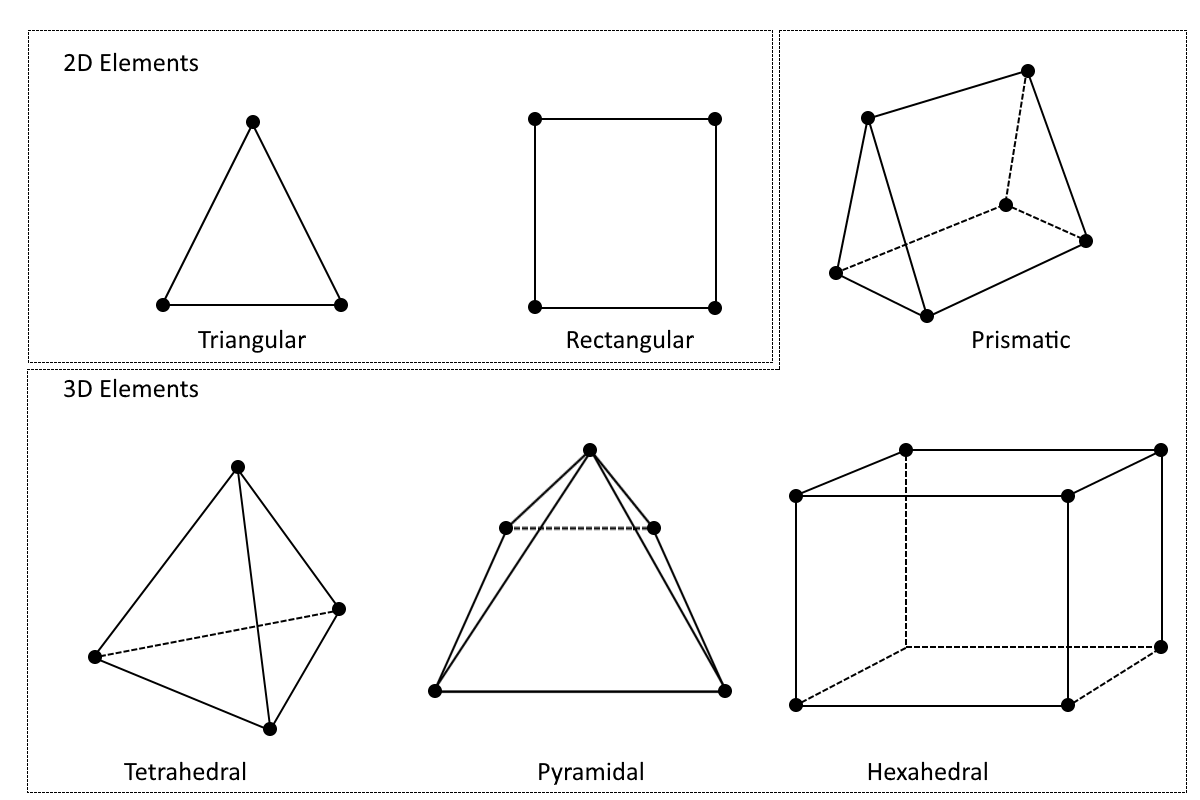
\includegraphics[width=0.75\textwidth]{mesh_elements.png}
  \caption{Some common mesh elements. Figure from COMSOL\cite{noauthor_detailed_nodate}.}
  \label{fig:mesh_elements}
\end{figure}

There are primarily four types of 3D mesh elements available - the tetrahedral, cuboid, prism, and pyramid.
Figure \ref{fig:mesh_elements} shows some common mesh elements.
These can be combined in various ways to represent any 3D geometry.
The most general 3D element is the tetrahedral and will approximate any geometry well.
However, it is not always the most effective choice for meshing a geometry and another element type may be better suited.
This is easiest illustrated with an example.\par

Imagine that you are trying to simulate the laminar flow of some fluid in a pipe.
Because of symmetry, only a wedge of the pipe needs to be explicitly modeled.
Therefore, in this scenario, it might be beneficial to use prism elements rather than tetrahedrals, since these are already wedge shaped.

The laminar pipe flow will have a gradient in the direction of the flow.
Thus the mesh mostly only needs to be fine in the flow direction, while the mesh can be coarser in the radial direction.
Constructing a mesh on this basis would allow us to achieve a solution of high accuracy while still keeping the number of elements relatively small - all through clever mesh design (see Figure \ref{fig:cylinder_mesh}).\par

\begin{figure}[htb!]
  \centering
  \begin{subfigure}{0.49\textwidth}
    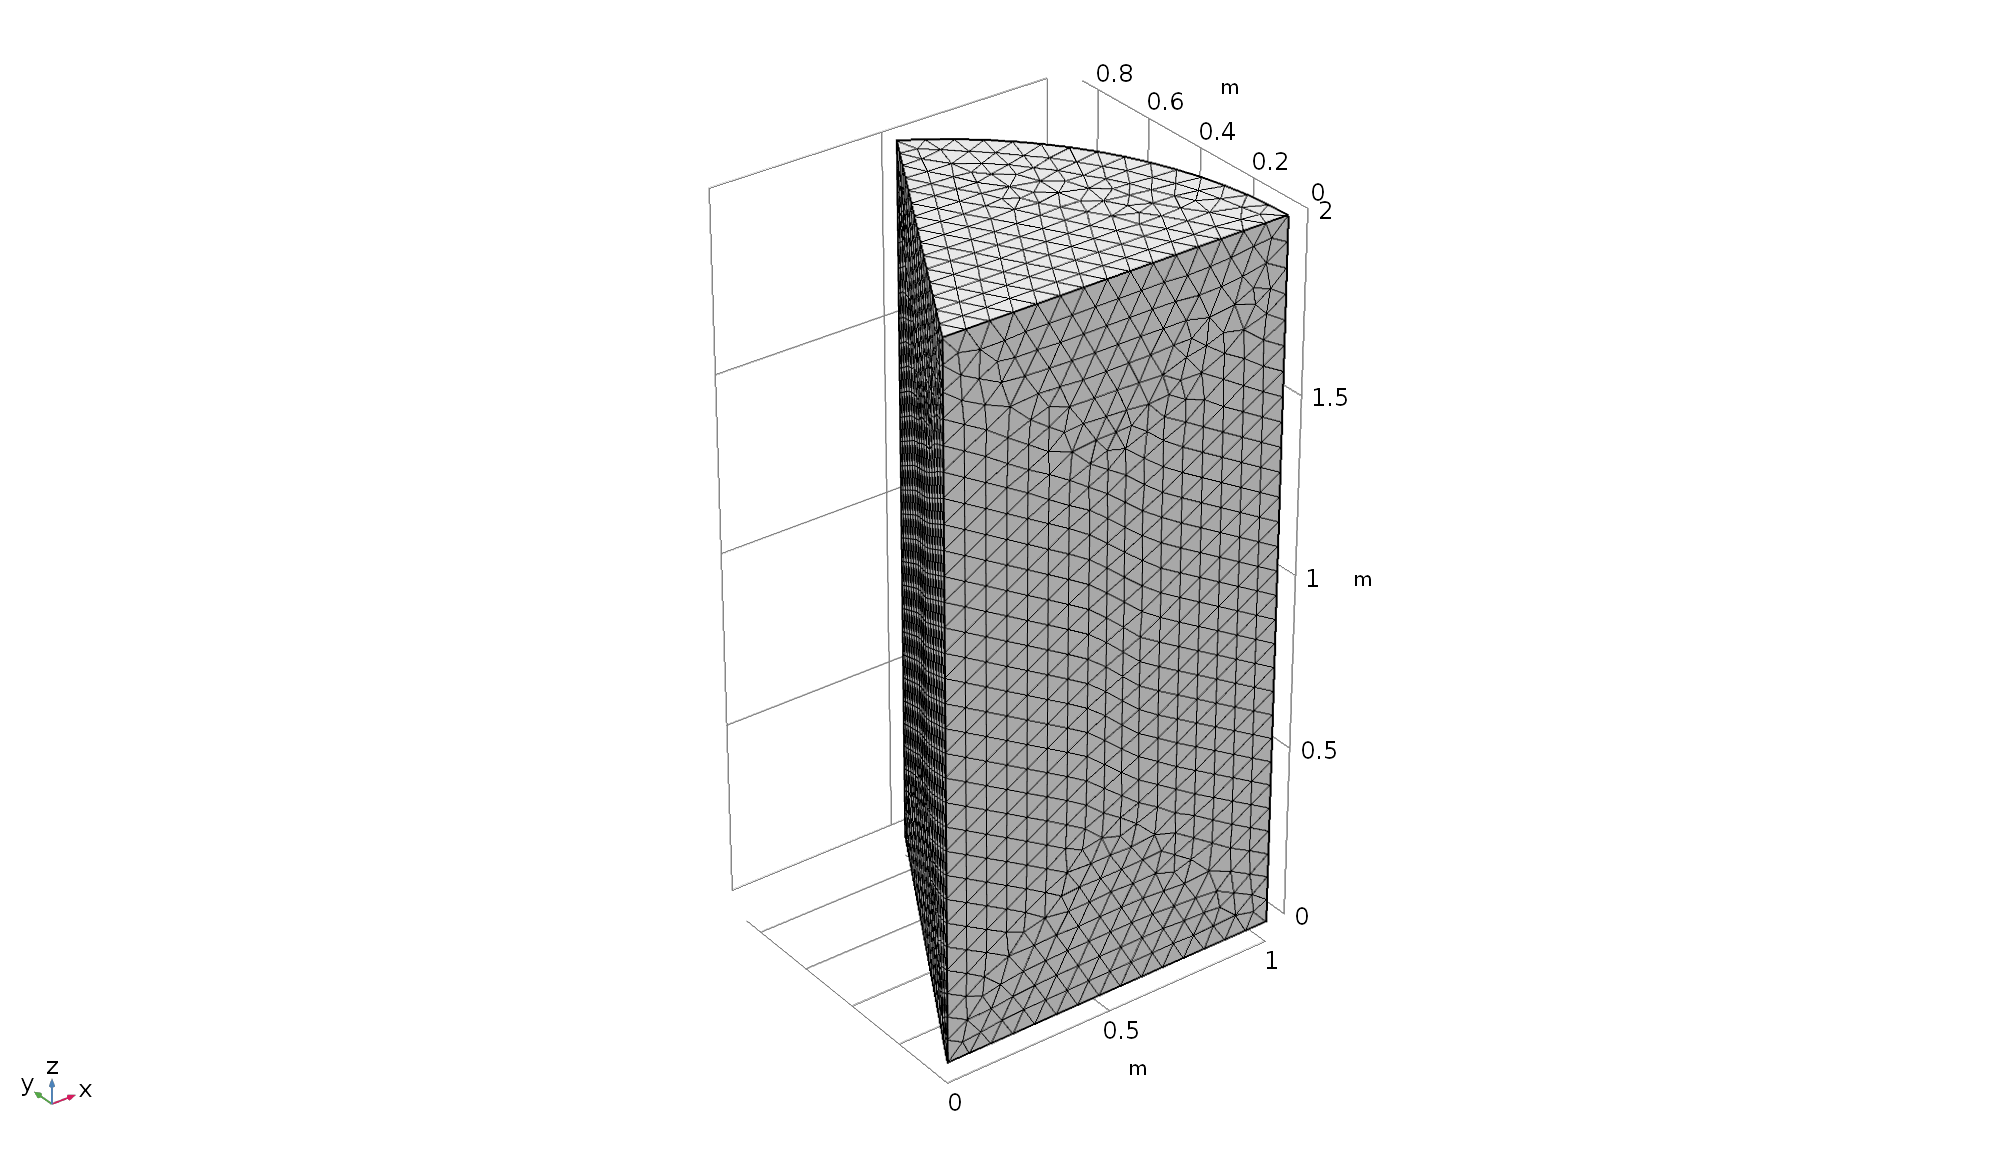
\includegraphics[width=\textwidth]{cylinder_regular_mesh.png}
  \caption{Mesh using tetrahedrals. 50,197 elements.}
  \end{subfigure}
  \begin{subfigure}{0.49\textwidth}
    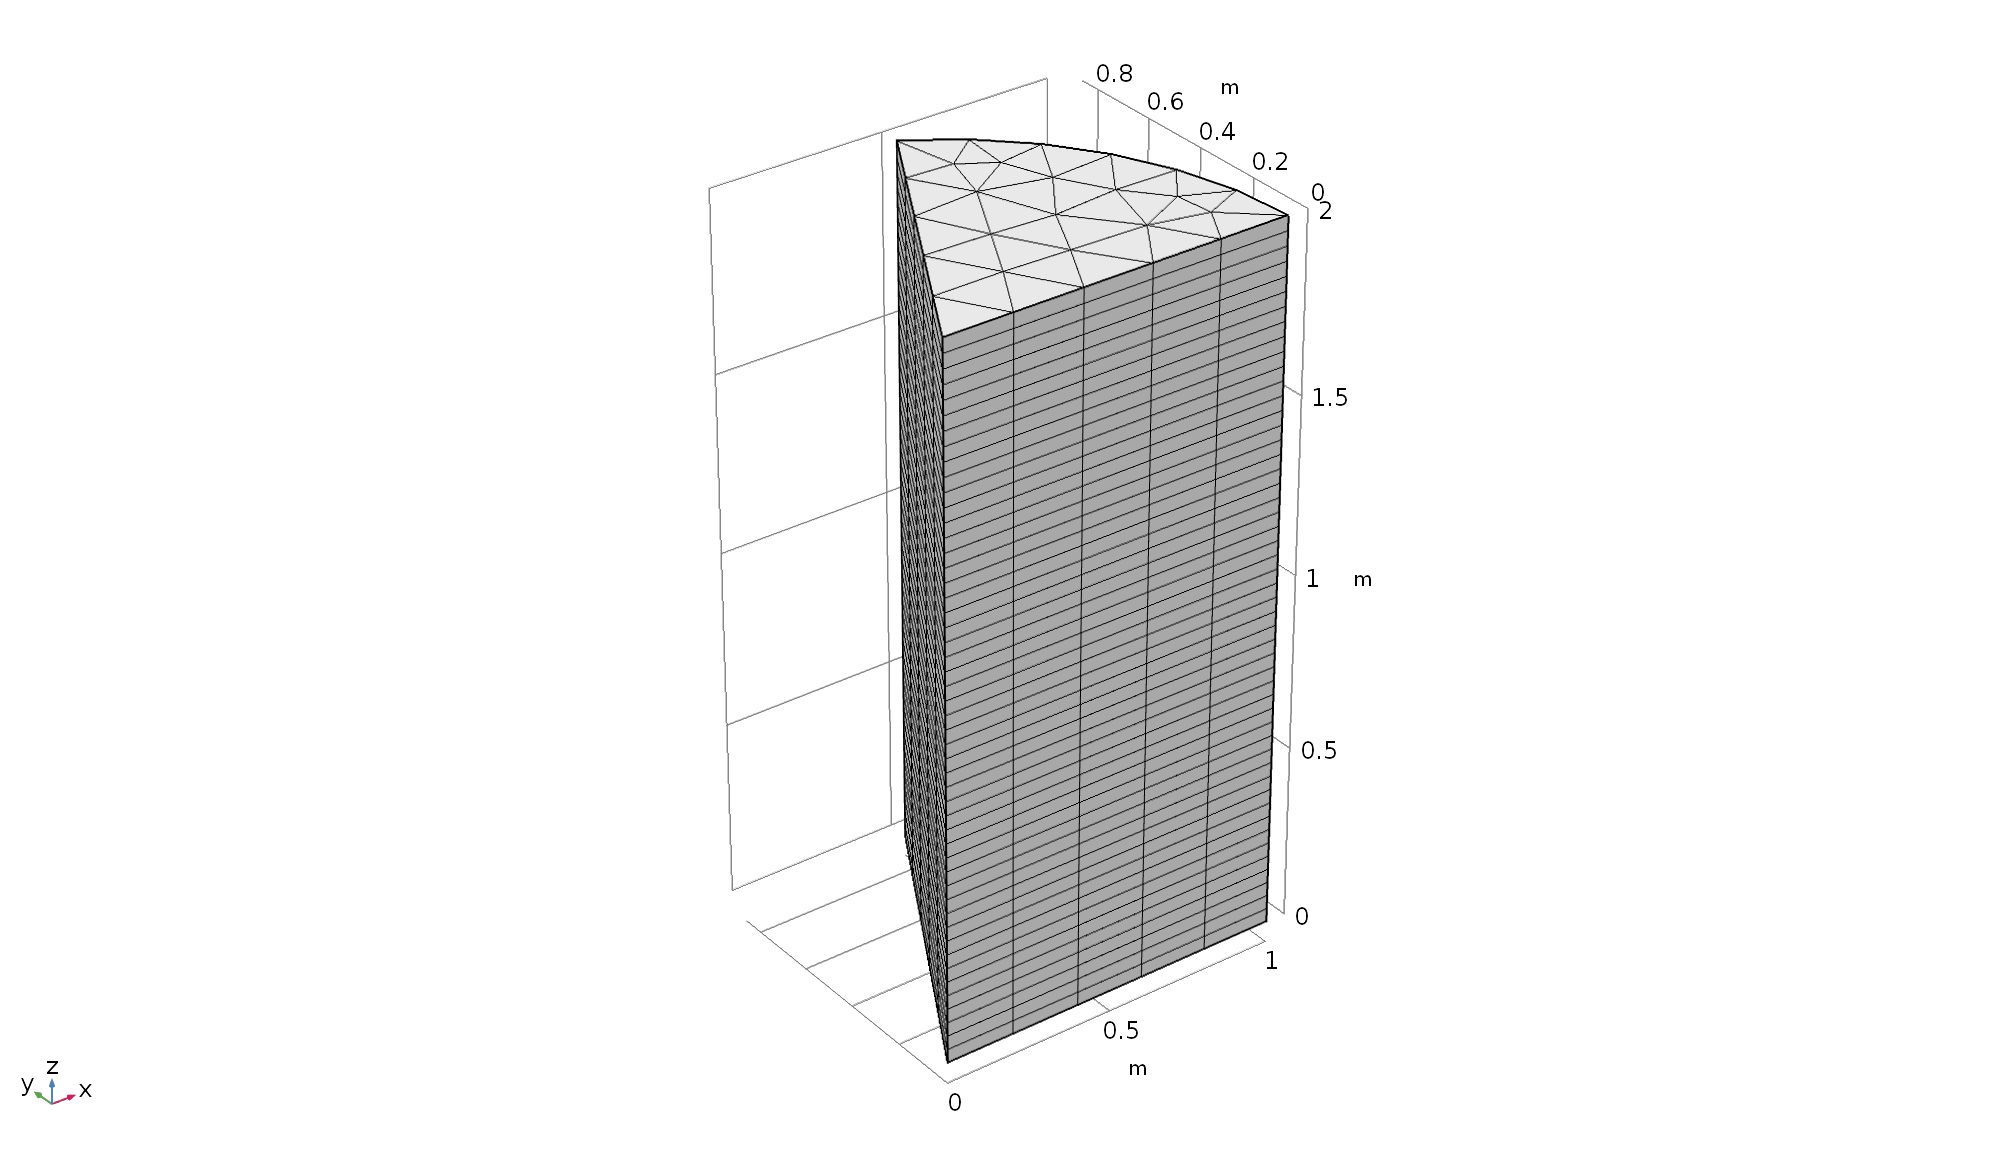
\includegraphics[width=\textwidth]{cylinder_swept_mesh.png}
  \caption{Mesh using prism elements. 1900 elements.}
  \end{subfigure}
  \caption[Example of how physical mesh design can reduce the number of elements.]{By understanding the physics, here considering laminar flow in a pipe (segment), clever mesh design can significantly reduce the number of mesh elements. Notice that the mesh density in the axial direction is more or less the same.}
  \label{fig:cylinder_mesh}
\end{figure}

This is of course a relatively simple example and more complicated geometries may need all kinds of element for constructing a clever design.
These type of multi-element meshes can give significant computational saving but at the expense of often requiring significant user input to be generated.
Sticking to one type of elements is often simpler as these can quickly and easily mesh geometries.\par

Meshing can be done manually, but is often performed by a meshing algorithm.
The creation of these algorithms is a science in itself, but their use often involve passing some basic parameters to the algorithm.
Here the user could, for instance, specify the maximum and minimum element sizes, maximum element growth rate, how finely small features or curves (typically quite difficult to mesh) should be meshed.
These instructions can be specific to various parts of the model, e.g. much finer meshing resolution can be specified for an area of interest and vice versa.
There are also a variety of specialty mesh features such as a mesh boundary layer available: adding finely spaced mesh layers along a boundary.
How to use all of these tools effectively to mesh a geometry is why meshing can be one of the most challenging aspects of FEM modeling.\par

\subsection{Meshing The VI Model}

The first choice we need to make is which type of element to use, and in order to do that we need to think about the gradients of the dependent variables.\par

From van Genuchten's retention curves, we know there will be a large soil moisture gradient in the capillary zone, which will need a relatively fine mesh to be resolved.
The airflow from Darcy's Law will forming some sort of arcing streamline from the ground surface to the foundation crack; the pressure gradient will be inline with these streamline.
The concentration gradient is difficult to predict a priori, but there likely will be some gradient from the groundwater to the ground surface and foundation crack.
Since many of these gradients intersect and go in different directions from each other it makes sense to use tetrahedral elements to mesh the geometry; these are the more general 3D elements.\par

Properly meshing our geometry can be a challenge due to the great range of geometric scale.
The house and soil domains are on the order of meters while the foundation crack is only \SI{1}{\centi\meter} side, and requires very fine meshing.
This is not only due to its small size, but because the contaminant entry will be calculated based on the solution here, which largely determines the indoor contaminant concentration.\par

The COMSOL meshing algorithm only require a few parameters to relatively mesh a geometry with tetrahedrals.
A description of each parameter and its value can be seen in Table \ref{tbl:meshing}.
\begin{table}[htb!]
  \begin{tabularx}{\linewidth}{l c X}
    \toprule
    Input & Value & Description \\
    \midrule
    Maximum element size & \SI{1.5}{\metre} & Maximum size of a element \\
    Minimum element size & \SI{1}{\milli\metre} & Minimum size of a element \\
    Maximum element growth rate & 1.3 & Maximum allowed size increase of adjacent elements. 1.3 indicates that an element can only be 30\% larger than its neighbor. A smaller value gives a finer mesh. \\
    Curvature factor & 0.4 & Ratio between the boundary element size and the geometry curvature radius. A smaller value gives a finer mesh. \\
    Resolution of narrow regions & 1 & Control the number of layers of elements that are created in narrow regions. A larger value gives a finer mesh. \\
    \bottomrule
  \end{tabularx}
  \caption{Inputs to COMSOLs meshing algorithm.}
  \label{tbl:meshing}
\end{table}

\subsection{Boundary Layer Mesh}

When posed with steep gradients in one particular direction at boundaries, as we have here, it is often useful to use a \textit{boundary layer mesh} at the impacted boundaries.
This is a type of mesh that introduces a dense layer of meshes along the normal direction from a boundary.
Boundary layer meshes are common features in meshing algorithms, and COMSOL's is no exception.\par

The number of boundary layers are supplied by the user, and in our case we will use 8 layers, but more could be added if needed.
The distance between each layer is determined by the size of the other elements in its vicinity, as well as the distance growth rate between each layer, which we set to 1.3, i.e. the distance increases by 30\% for each layer.
Figure \ref{fig:mesh} shows our completed mesh.\par

\begin{figure}[htb!]
  \centering
  \begin{subfigure}[b]{\textwidth}
    \centering
    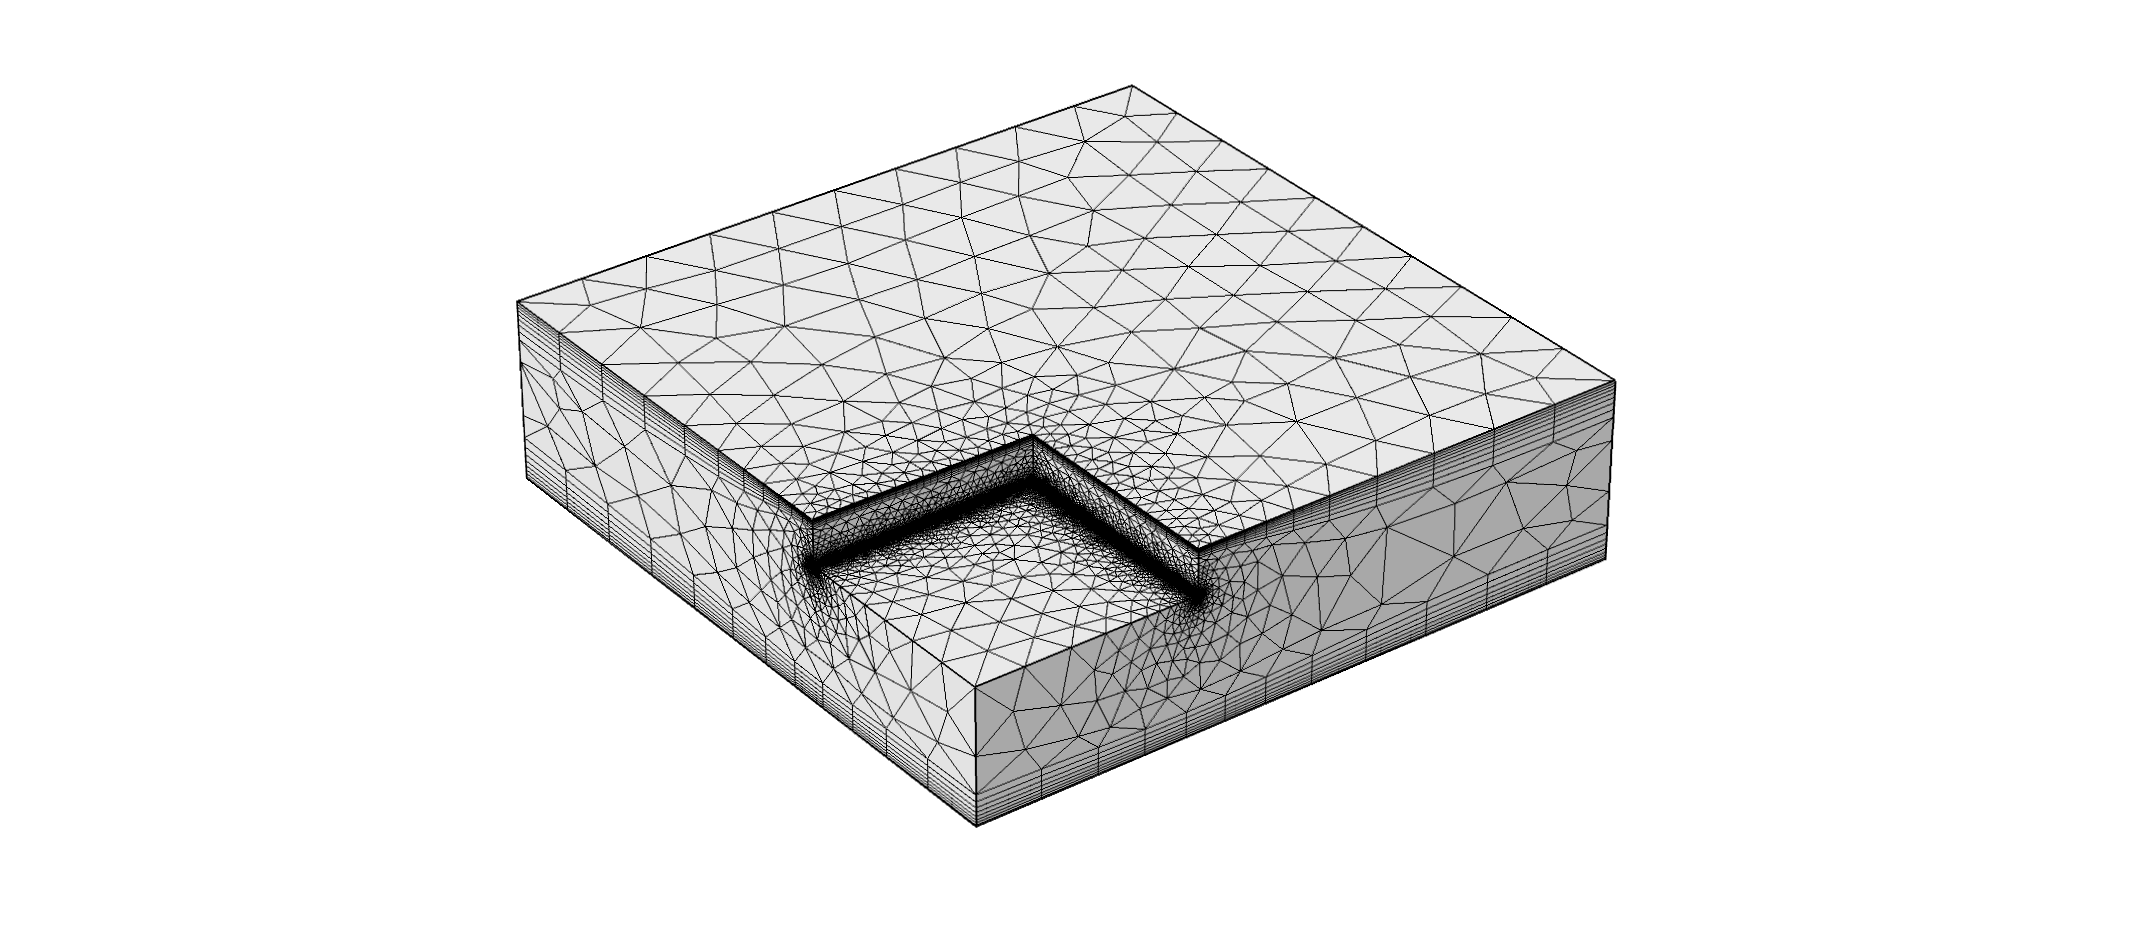
\includegraphics[width=0.75\textwidth]{meshed_model.png}
    \caption{The darker perimeter around the foundation highlights the higher mesh density along the foundation crack.}
    \label{fig:meshed_geometry}
  \end{subfigure}
  \begin{subfigure}[b]{\textwidth}
    \centering
    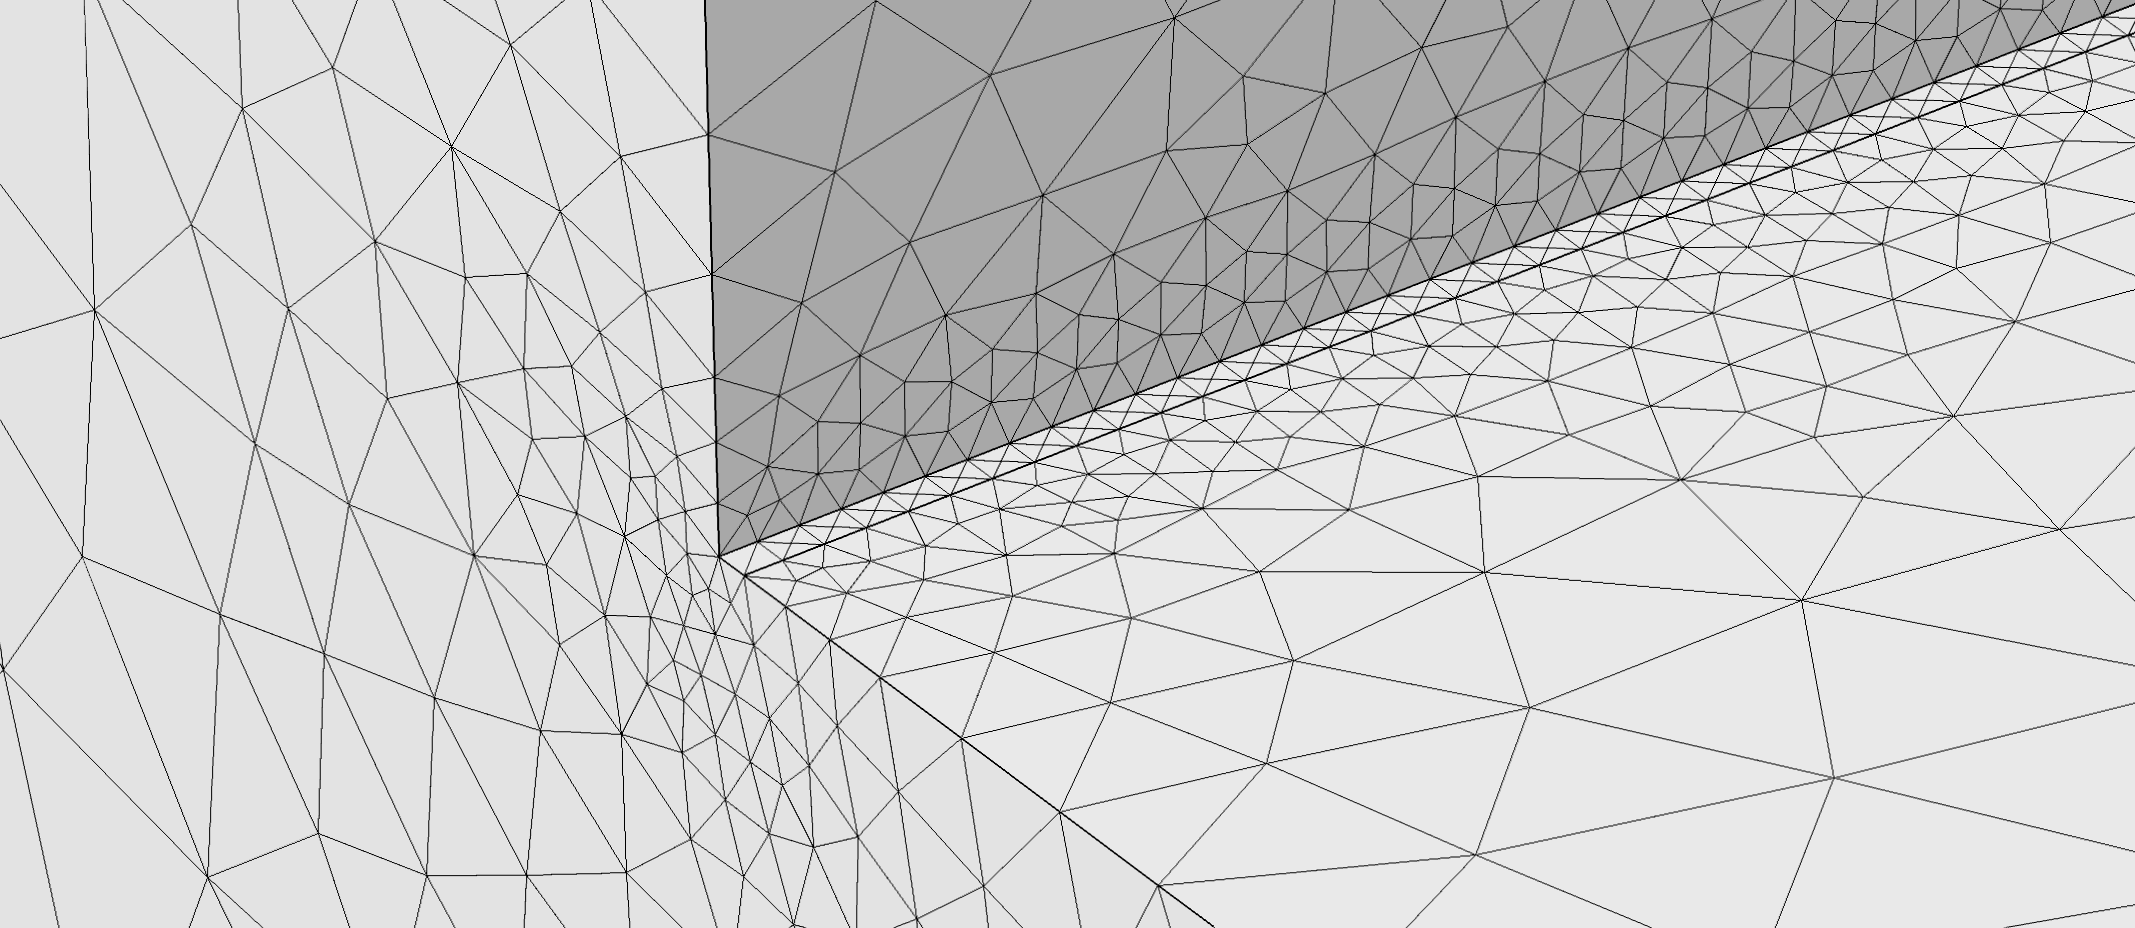
\includegraphics[width=0.75\textwidth]{mesh_crack.png}
    \caption{Close-up of the foundation crack mesh.}
    \label{fig:meshed_crack}
  \end{subfigure}
  \begin{subfigure}[b]{\textwidth}
    \centering
    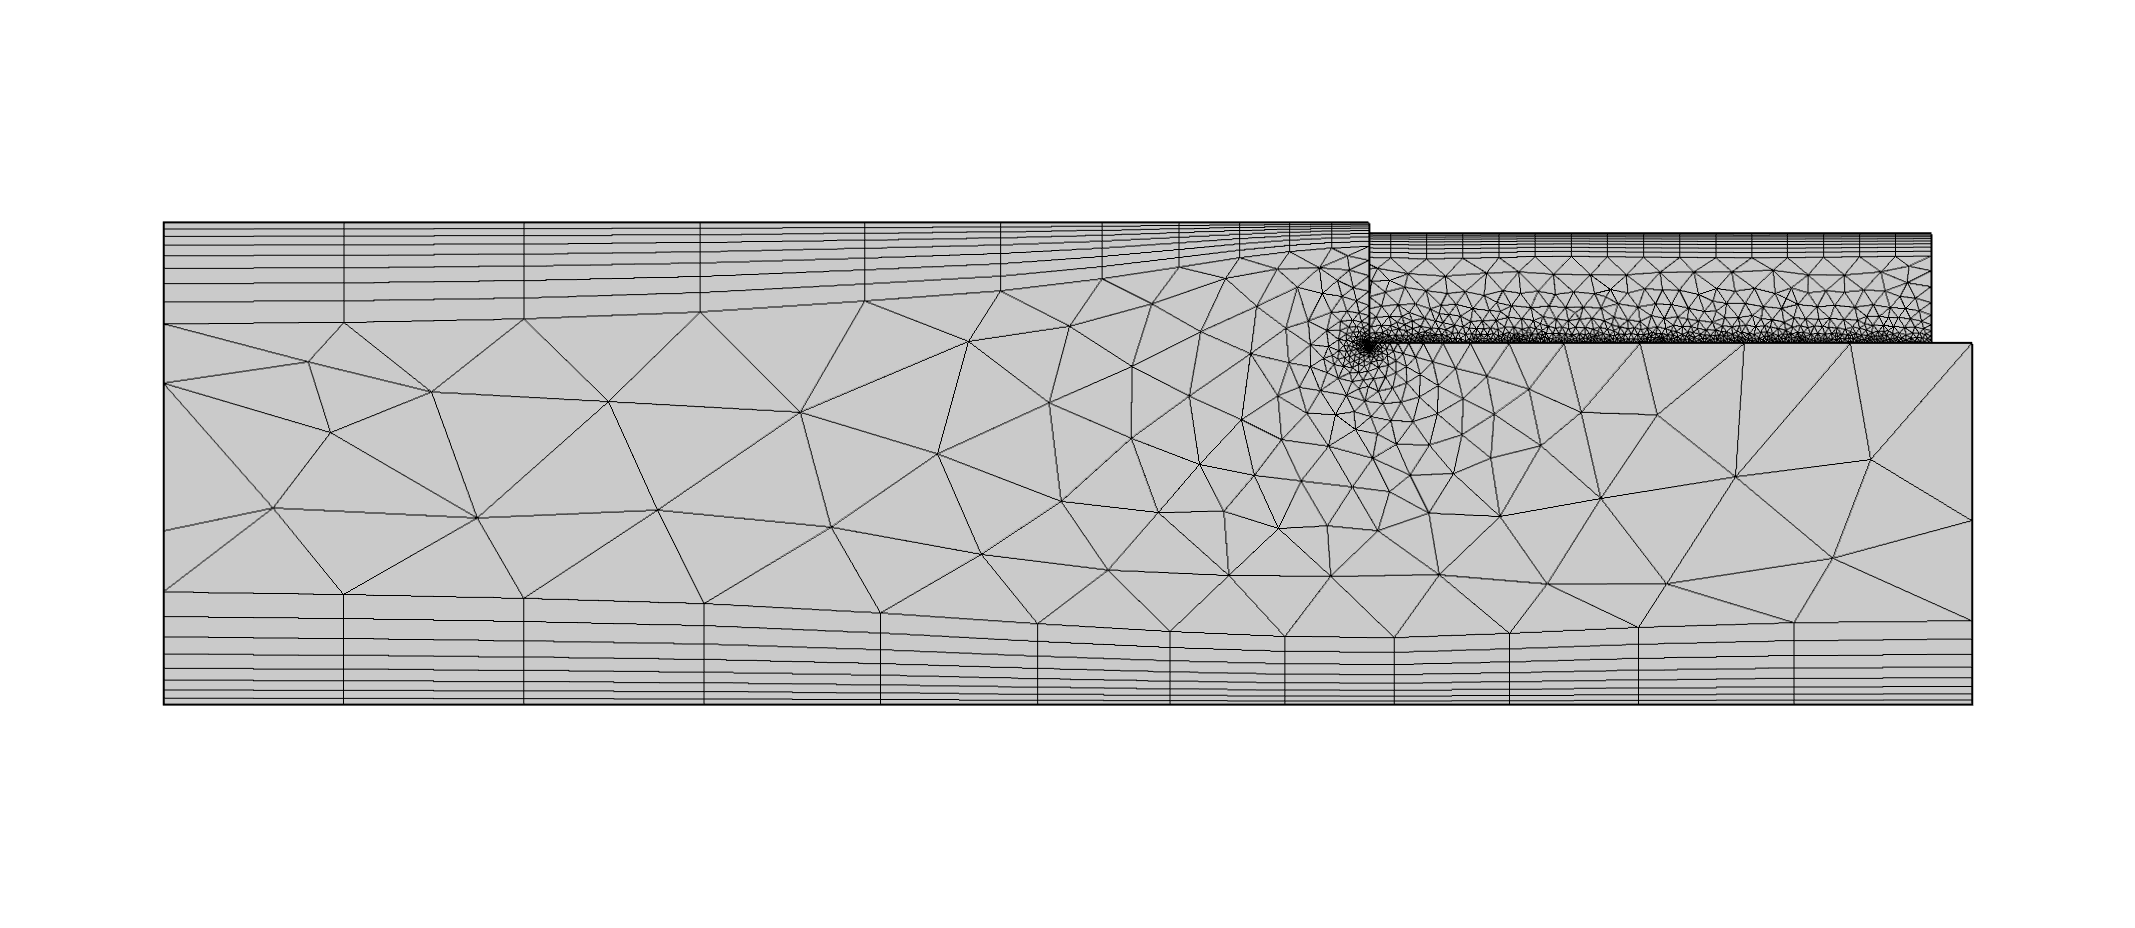
\includegraphics[width=0.75\textwidth]{mesh_boundary_layers.png}
    \caption{Side-view highlighting the boundary layer mesh.}
    \label{fig:mesh_boundary_layers}
  \end{subfigure}
  \caption[Initial finite element mesh of the modeled vapor intrusion scenario.]{Initial finite element mesh of the modeled vapor intrusion scenario.}
  \label{fig:mesh}
\end{figure}

\section{Solver Configuration}

A solver(s) is required to solve the VI model, and a few considerations need to be taken into account when choosing one.
For choosing and motivating a solver configuration, the \textit{COMSOL Multiphysics Reference Manual v5.3a}\cite{comsol_comsol_nodate} is here continuously used as a source.\par

For simplicity we will now first consider a stationary or steady-state problem.
Since our model is a multiphysics problem, i.e. many of the physical parameters depend on each other, we first need consider how to couple them.
They can be coupled by either using a \textit{segregated} or \textit{fully coupled} approach.\par

\paragraph{Segregated vs. fully coupled physics}

In a segregated solver, each governing equation is solved separately in a specific order.
For instance, in our VI example we can solve Darcy's Law first, get some solution for airflow in soil, and then use that velocity field in the transport equation, solve that, and then solve the indoor concentration equation, i.e. we solve one system equation per step.
These steps are simply iterated until convergence occurs in all of the separated steps.
In the case of VI calculations, the use of the segregated approach is fully justified because the concentrations of contaminant vapors are normally so low that they have no impact on the solution of soil airflow using Darcy's Law.
The fully coupled approach assembles a single large system of equations.
Both of these approaches should reach the same solution, but the fully coupled approach will do so faster, but at the expense of using more memory.\par

\paragraph{Direct vs. iterative solver}

Within each of these coupling approaches, we need to specify a solver to solve the system of equations.
Here we are again faced with a choice, and we could either use a \textit{direct} or \textit{iterative} solver.
Direct solvers, as the name implies, arrive at a solution directly and are based on LU-decomposition.
Iterative solvers on the other hand, iteratively approach the solution, and are based on conjugate gradient method.
The advantage of direct solvers is that they are faster, but use more memory, while iterative solvers are slower but use less memory.
In terms of choosing a solver algorithm, there are many options, but MUMPS and GMRES will be used as the respective algorithm for direct and iterative solvers.\par

\paragraph{Time-dependent solvers}

To solve a transient or time-dependent problem (which will be done in subsequent chapters) a solver to step forward in time is required.
Too large a time step will cause stability issues and ultimately convergence will be impossible, but obviously some discrete time step is required for a solution to be achievable.
A time-dependent solver picks an appropriate time-step and there are some popular approaches, such as using some high-order Runge-Kutta (RK) or backwards differentiation formula (BDF).
Regardless of the type of solver, for each time step the system of equations will be solved using one of the aforementioned solvers.
The difference between RK and BDF is that RK explicitly discretizes time while BDF does so implicitly.
In this work we will only use BDF as it is more stable than RK.\par

\paragraph{Choosing solvers}

The choice of solver will not affect (or should not at least) the solution to the problem.
However, it can have a large impact on computational time and resources, and these considerations dictate solver choice (this is also partially dependent on the mesh used, as this will affect memory usage too).
In this example, and throughout the models used in this work, we will favor speed over memory and therefore fully couple all our equations and use direct solvers.\par

\subsection{Adaptive Mesh Refinement}

The accuracy of the solution obtained by FEM is dependent on the quality of the mesh, something that was discussed in section \ref{sec:meshing}.
While the mesh designer can do much to create a mesh that performs well for the particular problem posed, refinement of the mesh is often needed and should be performed for every new model.\par

There are two types of mesh refinements in FEM.
The first type reduces the size of the elements and thereby the accuracy of the solution, this is called \textit{h-type} refinement ($h$ is often used to denote the mesh size).
The second increases the order of the polynomial of the basis function, called \textit{p-type} refinement which will likewise increases the solution accuracy.\par

h-type refinement is generally more attractive because it is simpler and the computational cost of p-type refinement increase faster than h-type.
However, p-types are useful if the user imports an already existing mesh, and is unable to change it, rendering h-type refinement impossible.
These two method can be combined to perform a \textit{hp-type} refinement.\par

Refinement is usually done by an algorithm, which is possible because FEM has the built-in ability to estimate the local error of the solution anywhere in the domain.
The downside with using an algorithm is that the user has little control over how the mesh is refined.
The user can also manually refine the mesh by solving the model and plot how some relevant metric converges as the mesh is refined.
This can be a very time consuming, and therefore algorithms are usually preferable; a hybrid solution is to manually alter the mesh after the algorithmic mesh refinement.\par

Refinement can either be done locally or globally.
Global refinement involves defining some singular metric that will be used to evaluate the quality of the mesh, e.g. one might use the total stress in a metal bar as a metric here.
In local refinement, one still has to define some metric for evaluating the quality of the refinement, but evaluation only occurs on a subset of the domain, e.g. the stress on just one boundary of the same metal bar.
In both approaches the elements that have the largest estimated local relative error are refined, but the exact details of the refinement can differ between specific refinement algorithms.
The local relative error is defined as the difference of the approximated solution $u_h$ from one mesh to another.
\begin{equation}\label{eq:rel_error}
  e = u_{h1} - u_h
\end{equation}
$e$ is the estimated local relative error (for every node);
$u_{h1}$ and $u_h$ are the approximated solutions on the refined and original meshes respectively.
The optimal type of refinement varies by problem, but a global refinement will generally be more computationally expensive.\par

\begin{figure}[htb!]
  \centering
  \begin{subfigure}[b]{\textwidth}
    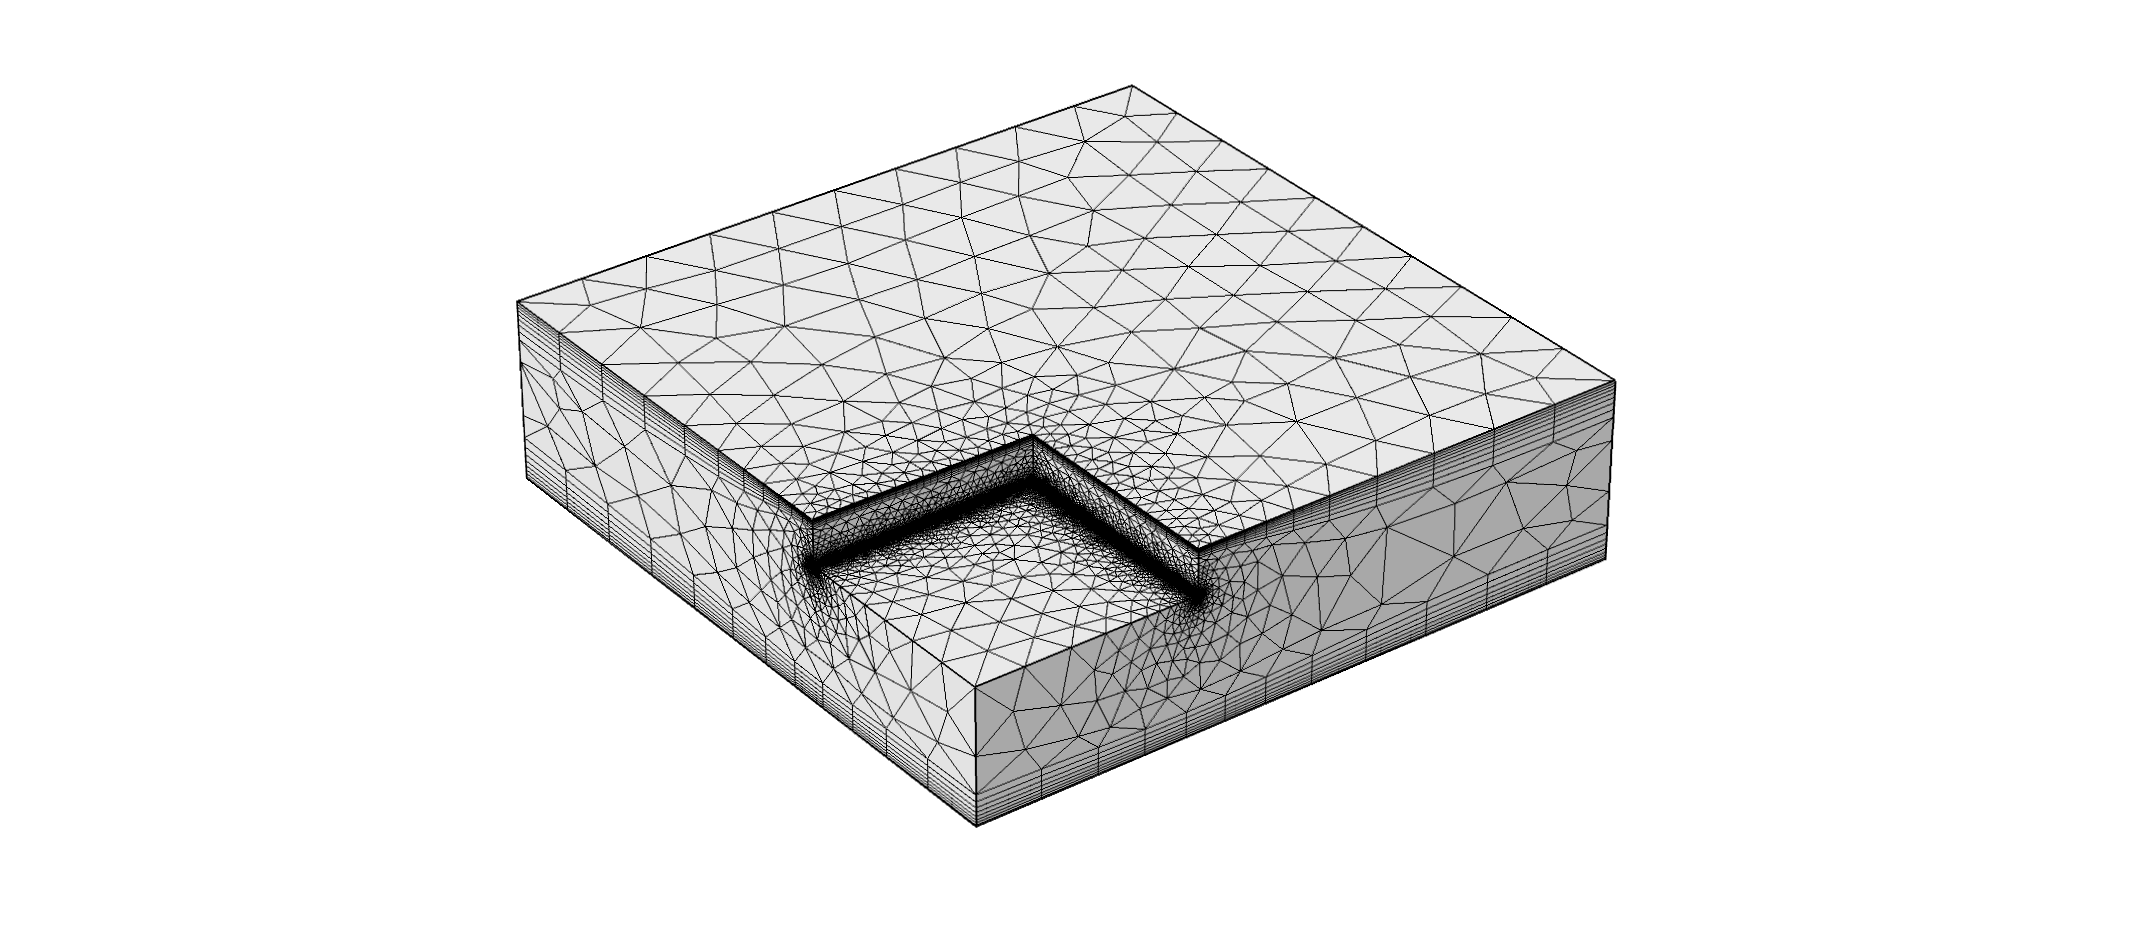
\includegraphics[width=\textwidth]{meshed_model.png}
    \caption{Original mesh. 362,657 elements.}
    \label{fig:mesh_before_refinement}
  \end{subfigure}
  \begin{subfigure}[b]{\textwidth}
    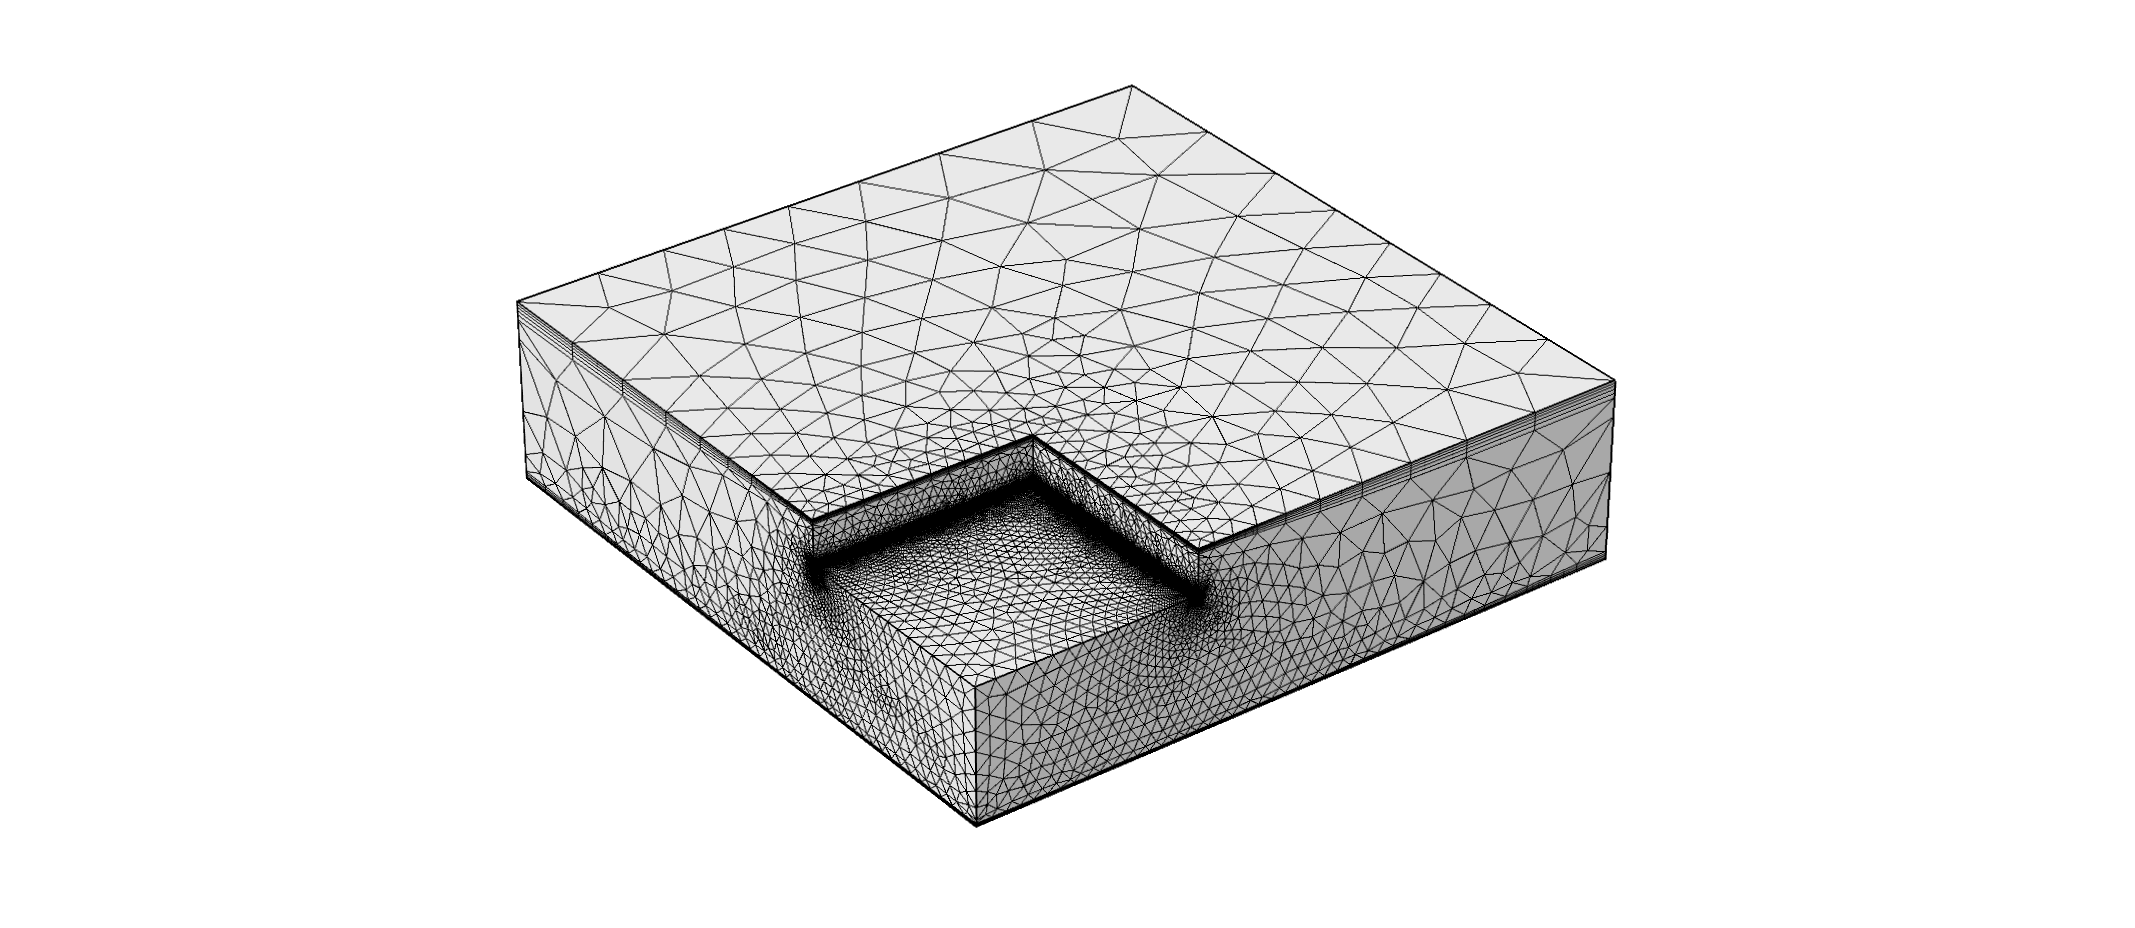
\includegraphics[width=\textwidth]{mesh_refined.png}
    \caption{Refined mesh after global refinement w.r.t. the indoor contaminant concentration. 1,065,743 elements.}
    \label{fig:mesh_after_refinement}
  \end{subfigure}
    \caption[Original and adaptatively refined mesh.]{Original and adaptatively refined mesh.}
    \label{fig:mesh_refinement_mesh}
\end{figure}

In this work we will use a global h-type refinement and use the indoor contaminant concentration $c_{in}$ as our refinement metric.
COMSOLs refinement algorithm has the nice ability to reinitialize the mesh, and can thereby coarsen elements, i.e. increase $h$ where the local error is very small.
This is handy as a fine mesh is not needed far away from the foundation crack - saving computational resources.
In this example we will tell the algorithm to refine the mesh three times, and stop if the total number of elements exceed 1 million, with a maximum coarsening factor of 3, and element growth rate of 1.3, i.e. the number of elements increase by roughly 70\% each iteration.\par

The result of this refinement can be seen in Figure \ref{fig:mesh_refinement_mesh} where the original and refined mesh are juxtaposed.
Notice how the mesh is now denser near the foundation, the boundary layers tighter (in particular near the groundwater boundary), and how the elements are larger in the periphery.
The original and refined meshes has 362,657 and 1,065,743 elements respectively.\par
Figure \ref{fig:mesh_refinement} shows how the value of $c_\mathrm{in}$ converges for each mesh refinement iteration.
What is plotted is the change in calculated indoor contaminant concentration with iteration.
Initially, very large changes are seen in the predicted values with the first iterations.
By the \nth{4} iteration, the improvements in estimates are getting very small.\par

\begin{figure}[htb!]
  \centering
  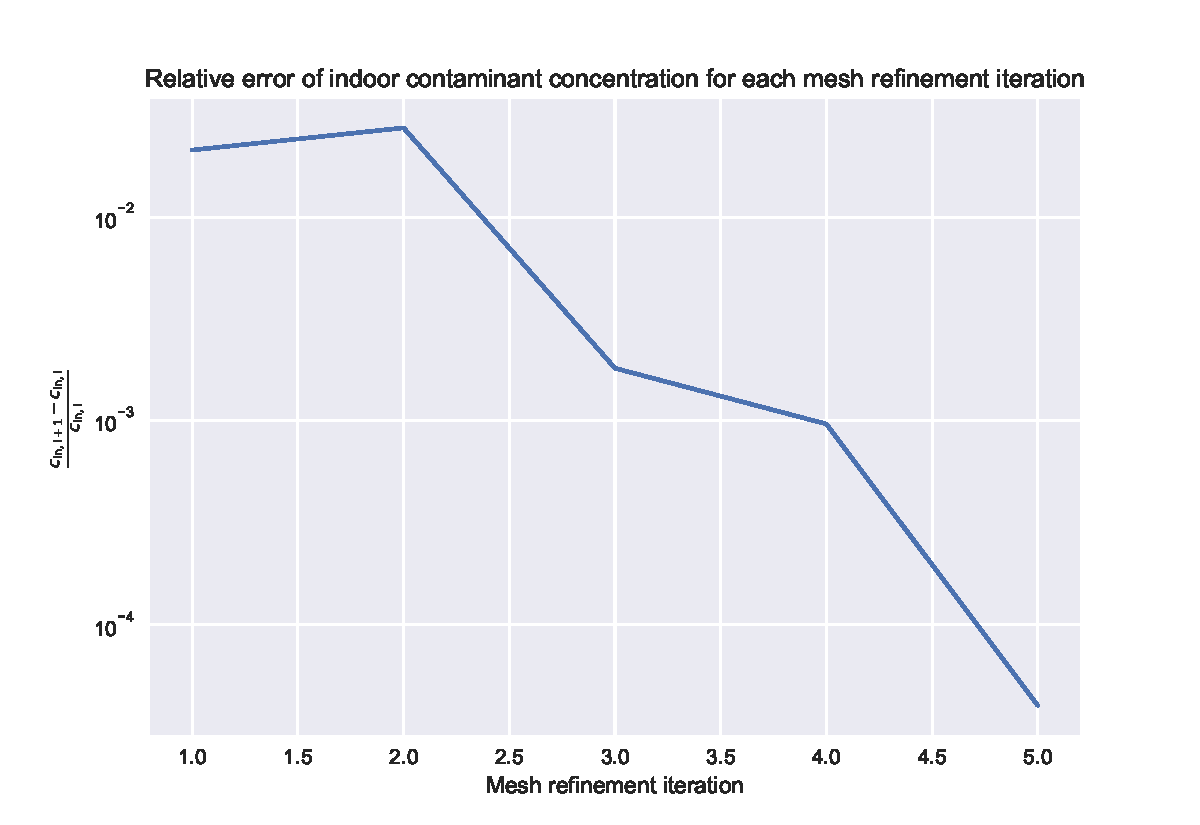
\includegraphics[width=0.75\textwidth]{mesh_refinement_error.pdf}
  \caption{Convergence of indoor air contaminant concentration as the mesh is refined.}
  \label{fig:mesh_refinement}
\end{figure}

\section{Post-processing \& Results}

One of the benefits of using a FEM software like COMSOL is its advanced post-processing capabilities.
This allows the user to examine the physics driving VI in great detail.
Figure \ref{fig:model_pressure} shows the resulting pressure field from solving Darcy's Law, as well as the associated airflow streamlines in the soil.
Here we see the pressure in the near foundation crack region is roughly the same as the house pressurization of \SI{-5}{\pascal}, which quickly decreases towards the ground surface.
It is also apparent how this pressure field induces a airflow from the ground surface, with air near the house heading relatively straight to the foundation crack, whereas the air further away from the house penetrates deeper into the soil and almost "whirlwinds" underneath the house.\par

\begin{figure}[htb!]
  \centering
  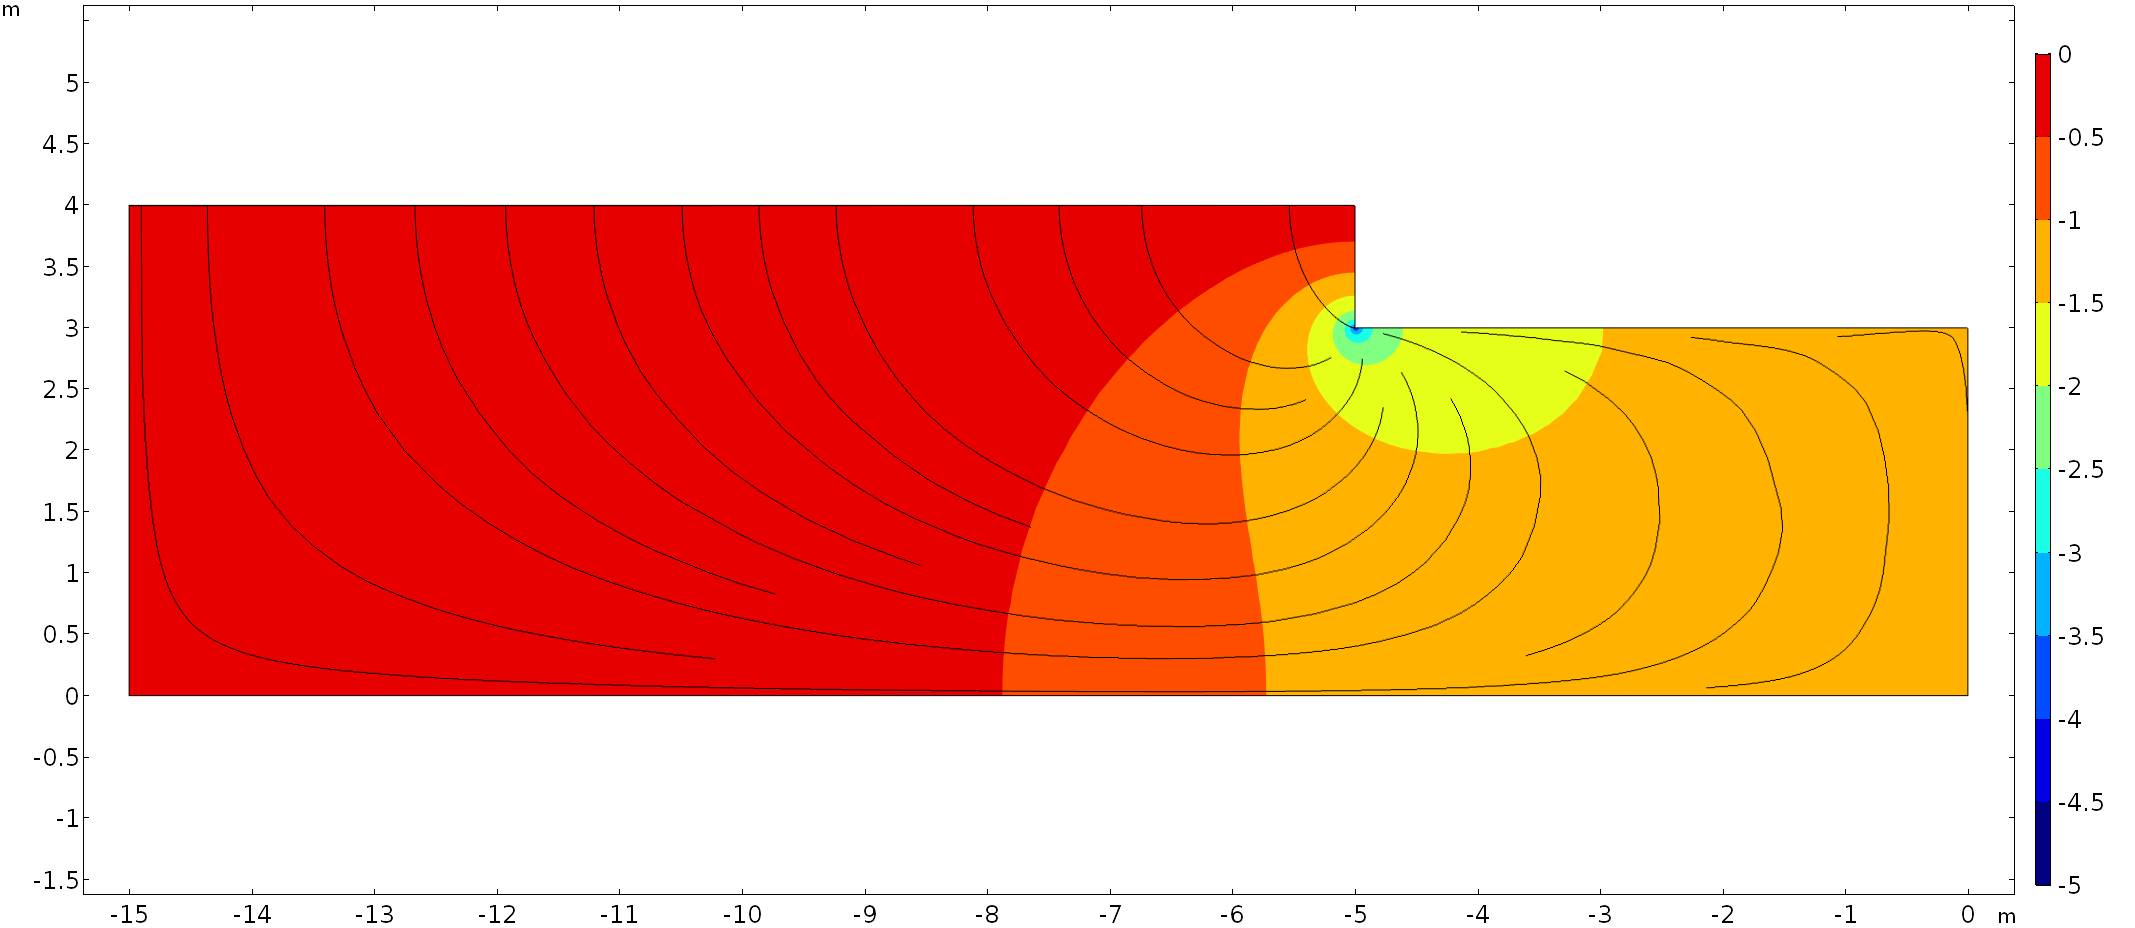
\includegraphics[width=0.75\textwidth]{model_pressure.png}
  \caption{Pressure field from Darcy's Law with associated airflow streamlines.}
  \label{fig:model_pressure}
\end{figure}

\begin{figure}[htb!]
  \centering
  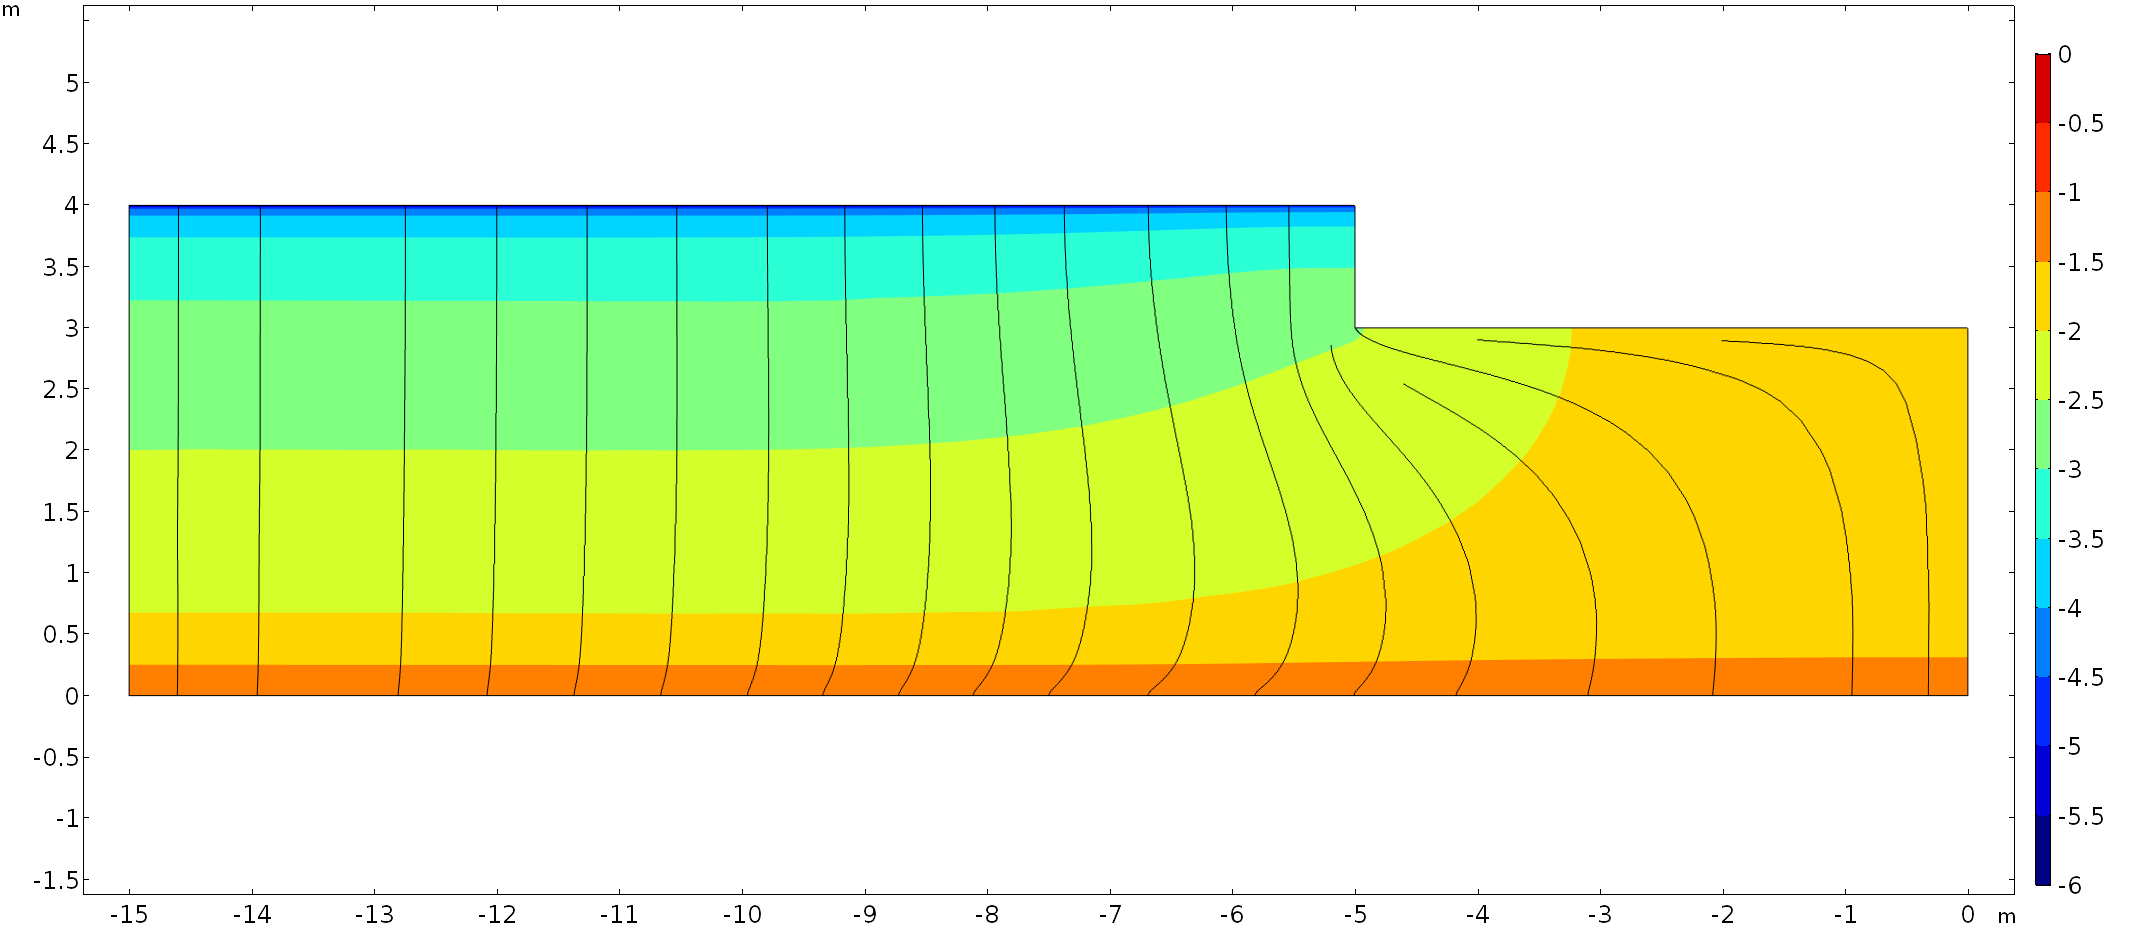
\includegraphics[width=0.75\textwidth]{model_concentration.png}
  \caption{Contaminant concentration in the soil, normalized to groundwater concentration and log-transformed, with transport streamlines.}
  \label{fig:model_concentration}
\end{figure}

The contaminant concentration in the soil, normalized to the groundwater source concentration and log-transformed, with the contaminant flux streamlines, is examined in Figure \ref{fig:model_concentration}.
Here see that far away from the house, the contaminant vapor simply diffuse straight from the groundwater source to the atmosphere, while these accumulate underneath the house, which acts as a diffusion blocker.
Based on those streamlines we can conclude that the advective component of the flux is very here small.
Perhaps surprisingly, we do not see a significant advective transport downwards along the wall of the house.
However, considering that the soil type is sandy loam, airflow velocities are expected to be small.\par

One might think that advective transport is large in the horizontal direction along the foundation slab, as the transport and airflow streamlines are so similar.
However, by inspecting Figure \ref{fig:model_velocity_crack} we see that airflow velocities are not greater here than elsewhere, and therefore the advective transport is not either.
To make sense of this, we can inspect the horizontal diffusive flux, divided by the magnitude of the total flux
\begin{equation}
  \frac{j_\mathrm{diff,y-direction}}{|j_\mathrm{total}|}
\end{equation}
to see what portion of the total transport the diffusive horizontal represents here.
The results of this is shown in Figure \ref{fig:model_horizontal_diff}, where see that the horizontal diffusive flux in the left direction accounts for 80\% of the total flux magnitude, as indicated by -0.8. % TODO Explain this better
This shows the power of modeling and how it can reveal things that at first seem intuitively correct, but in fact are not.\par

\begin{figure}[htb!]
  \centering
  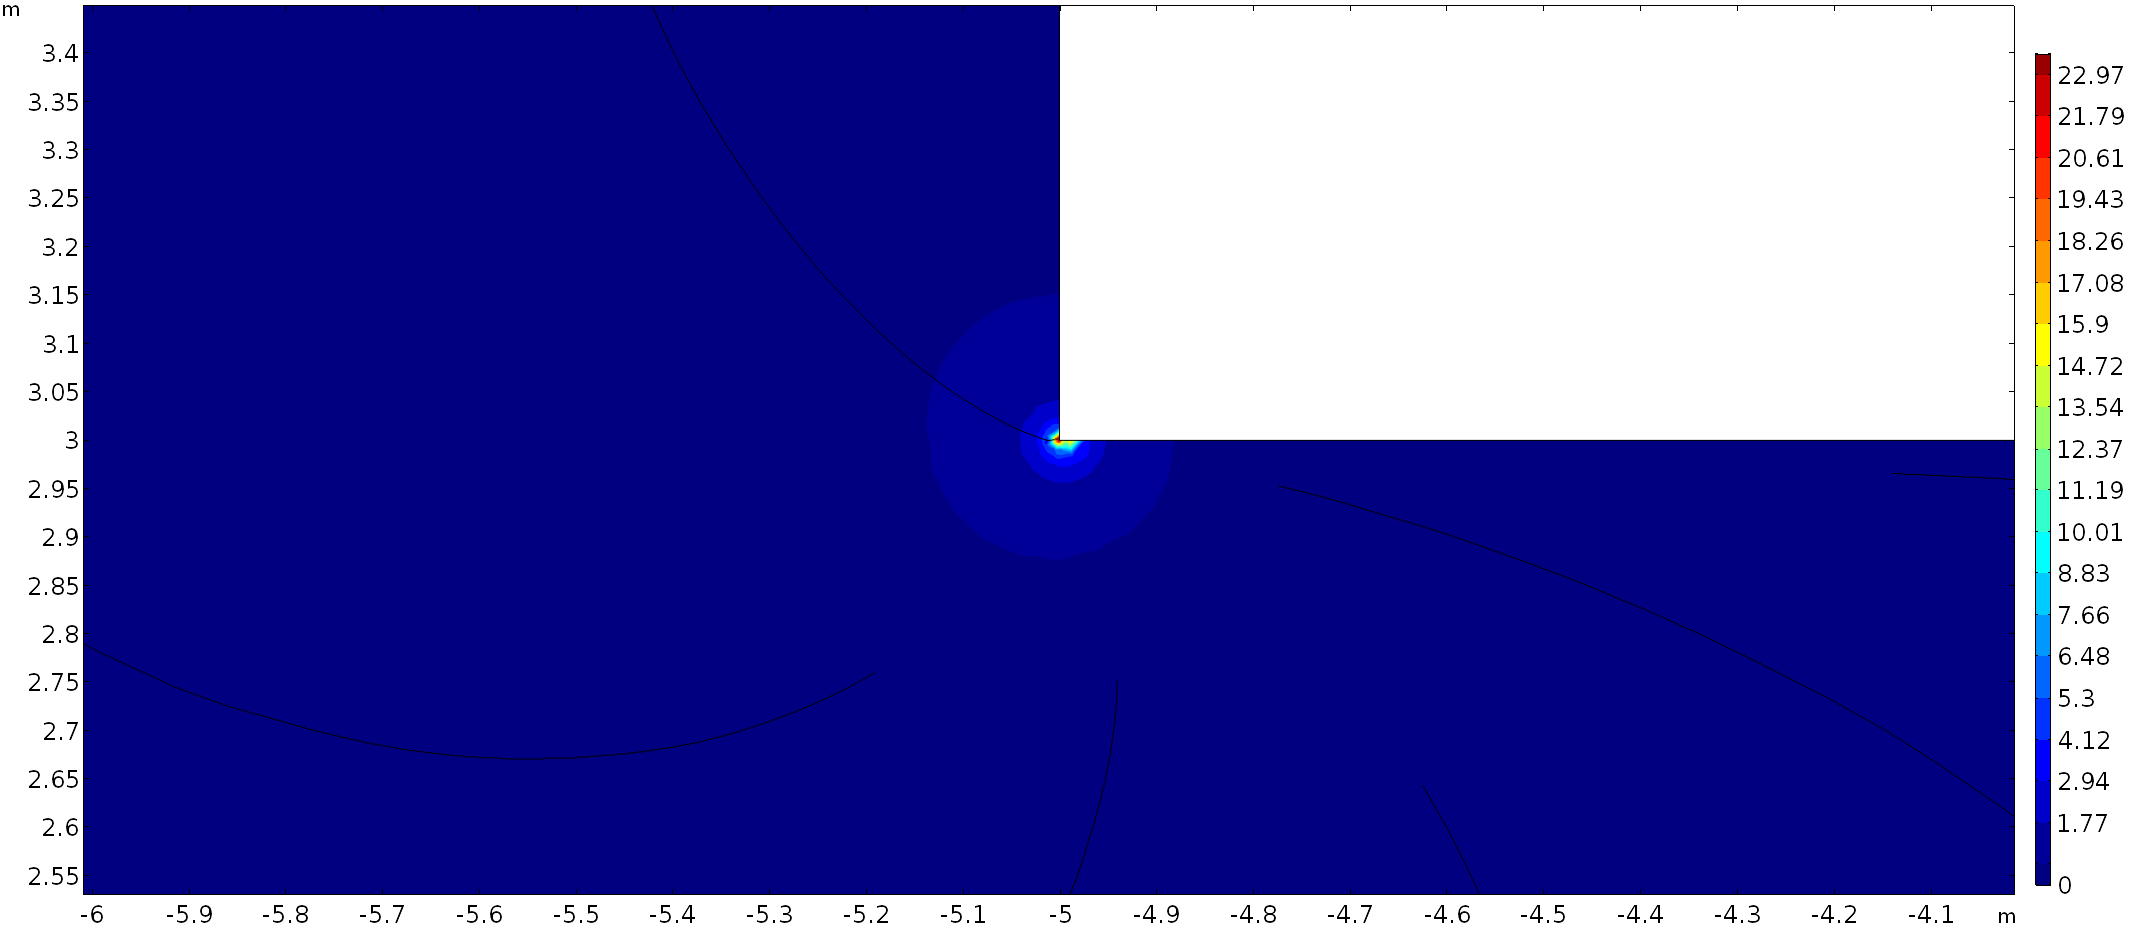
\includegraphics[width=0.75\textwidth]{model_velocity_crack.png}
  \caption{Airflow velocity [\si{\milli\metre\per\hour}] near the foundation crack with associated its streamlines.}
  \label{fig:model_velocity_crack}
\end{figure}

\begin{figure}[htb!]
  \centering
  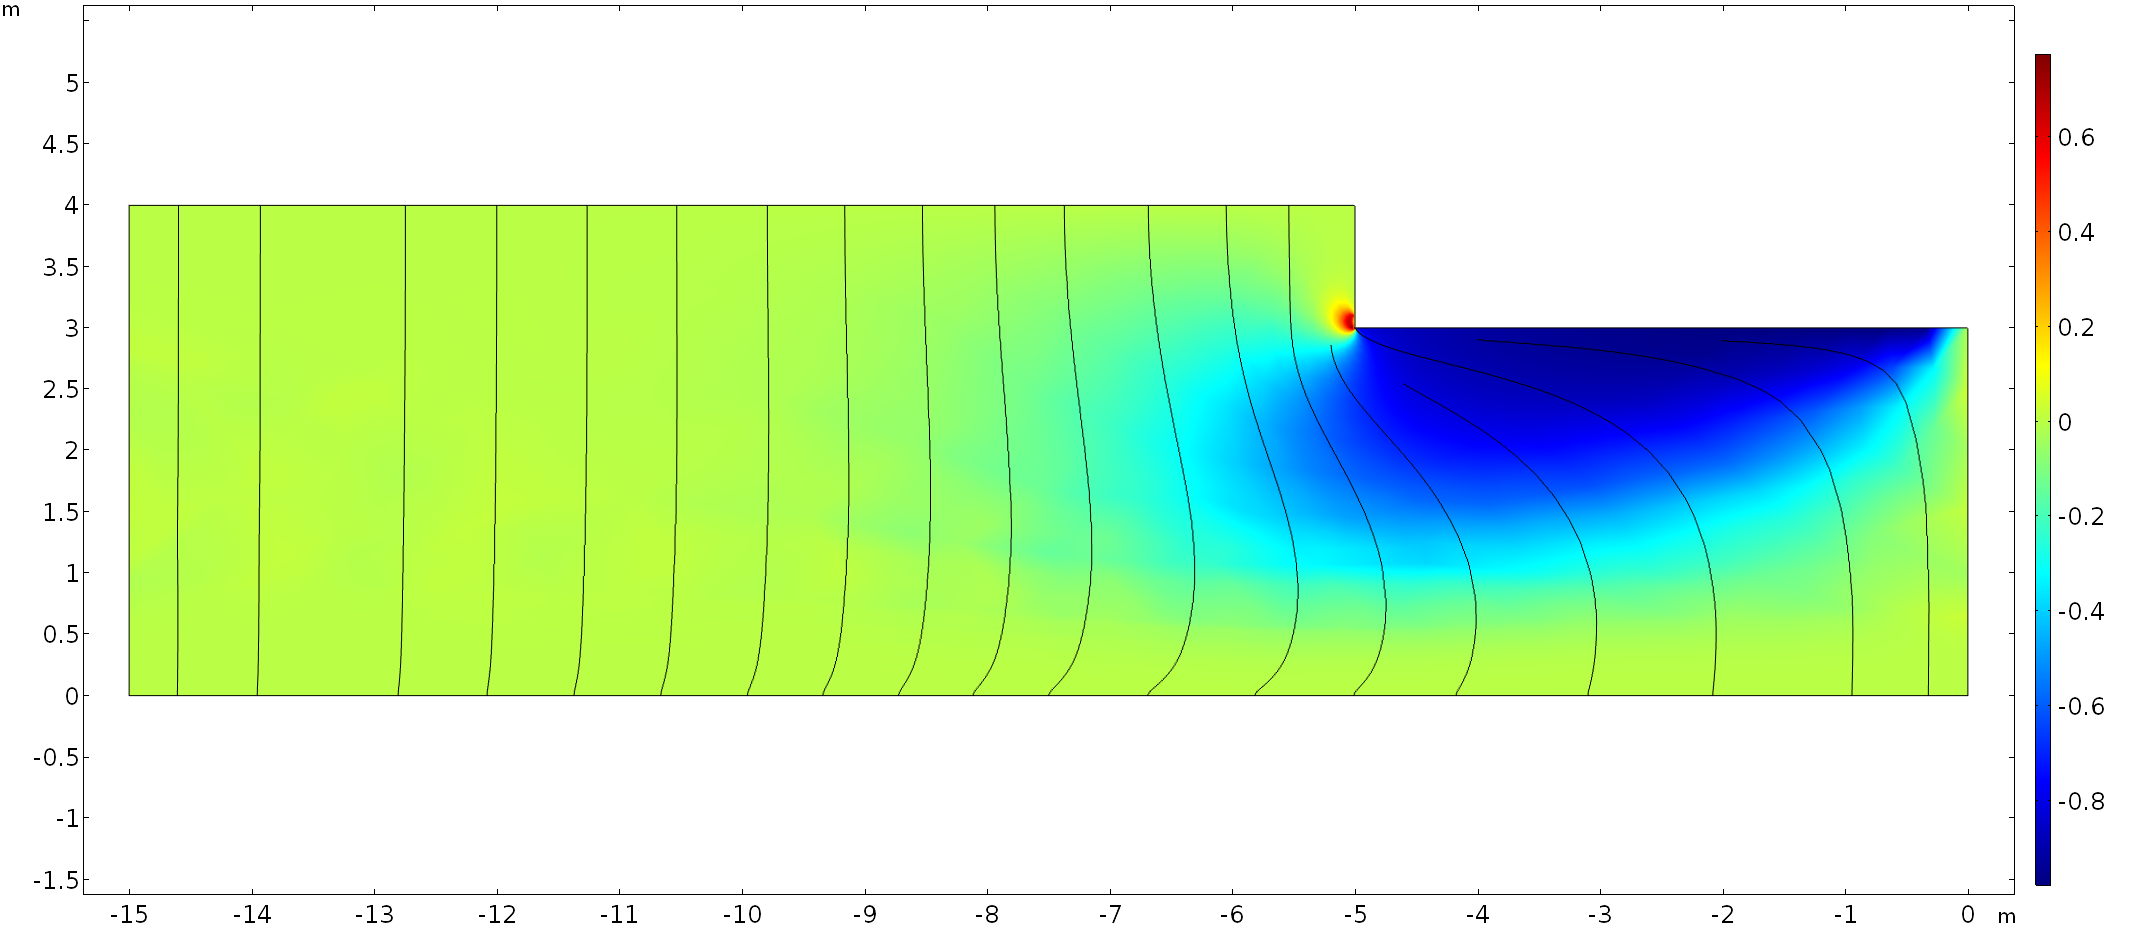
\includegraphics[width=0.75\textwidth]{model_transport_flux_y.png}
  \caption{Horizontal diffusive flux component of the magnitude of the total flux. 1 here would indicates that all of the contaminant transport is due to diffusion, and occurs solely in the rightwards direction.}
  \label{fig:model_horizontal_diff}
\end{figure}

Another useful feature of post-processing is that it can be used for bug searching and to evaluate where the mesh can be potentially improved.
When the transport equation is used to numerically model contaminant transport, there is a tendency for the solution to oscillate around the "true" solution, and thereby violate mass conservation, if the mesh size in a particular element is too large.
This can be quantified by the cell Péclet number, which characterizes the relative magnitude of advection/diffusion in a cell.
\begin{equation}
  \mathrm{Pe_{cell}} = \frac{\mathrm{adv_{cell}}}{\mathrm{diff_{cell}}} = \frac{u_g h}{2 D_\mathrm{eff}}
\end{equation}
here $u_g$ [\si{\metre\per\second}] is the soil-gas airflow velocity;
$h$ [\si{\metre}] is the mesh size in the element or cell;
and $D_\mathrm{eff}$ [\si{\metre\squared\per\second}] is the effective diffusivity in the cell.
If $\mathrm{Pe_{cell}} > 1$ there is a risk that this oscillating behavior will manifest.
Small exceedances, $~\mathrm{Pe_{cell}} < 25$, are usually mitigated by various stabilization schemes, which are inherently integrated into COMSOL as well as many other FEM packages, but for larger values further mesh refinement may be required.\par

Figure \ref{fig:model_cell_peclet} shows $\mathrm{Pe_{cell}}$ as a volume plot, and excludes all values that fall below one.
As we can see, only the region close to the groundwater exceeds $\mathrm{Pe_{cell}}$, which is due to the very small $D_\mathrm{eff}$ there.
The exceedance is small, so the stabilization scheme is able to compensate which is confirmed by Figure \ref{fig:model_concentration} (no oscillations visible).
This is also a region where even if such oscillations occurred, would probably not affect the indoor contaminant concentration.
Regardless, Figure \ref{fig:model_cell_peclet} shows where the mesh may potentially be refined, which comes in handy to know if one runs a model where airflow velocities are significantly higher than in this example.\par

\begin{figure}[htb!]
  \centering
  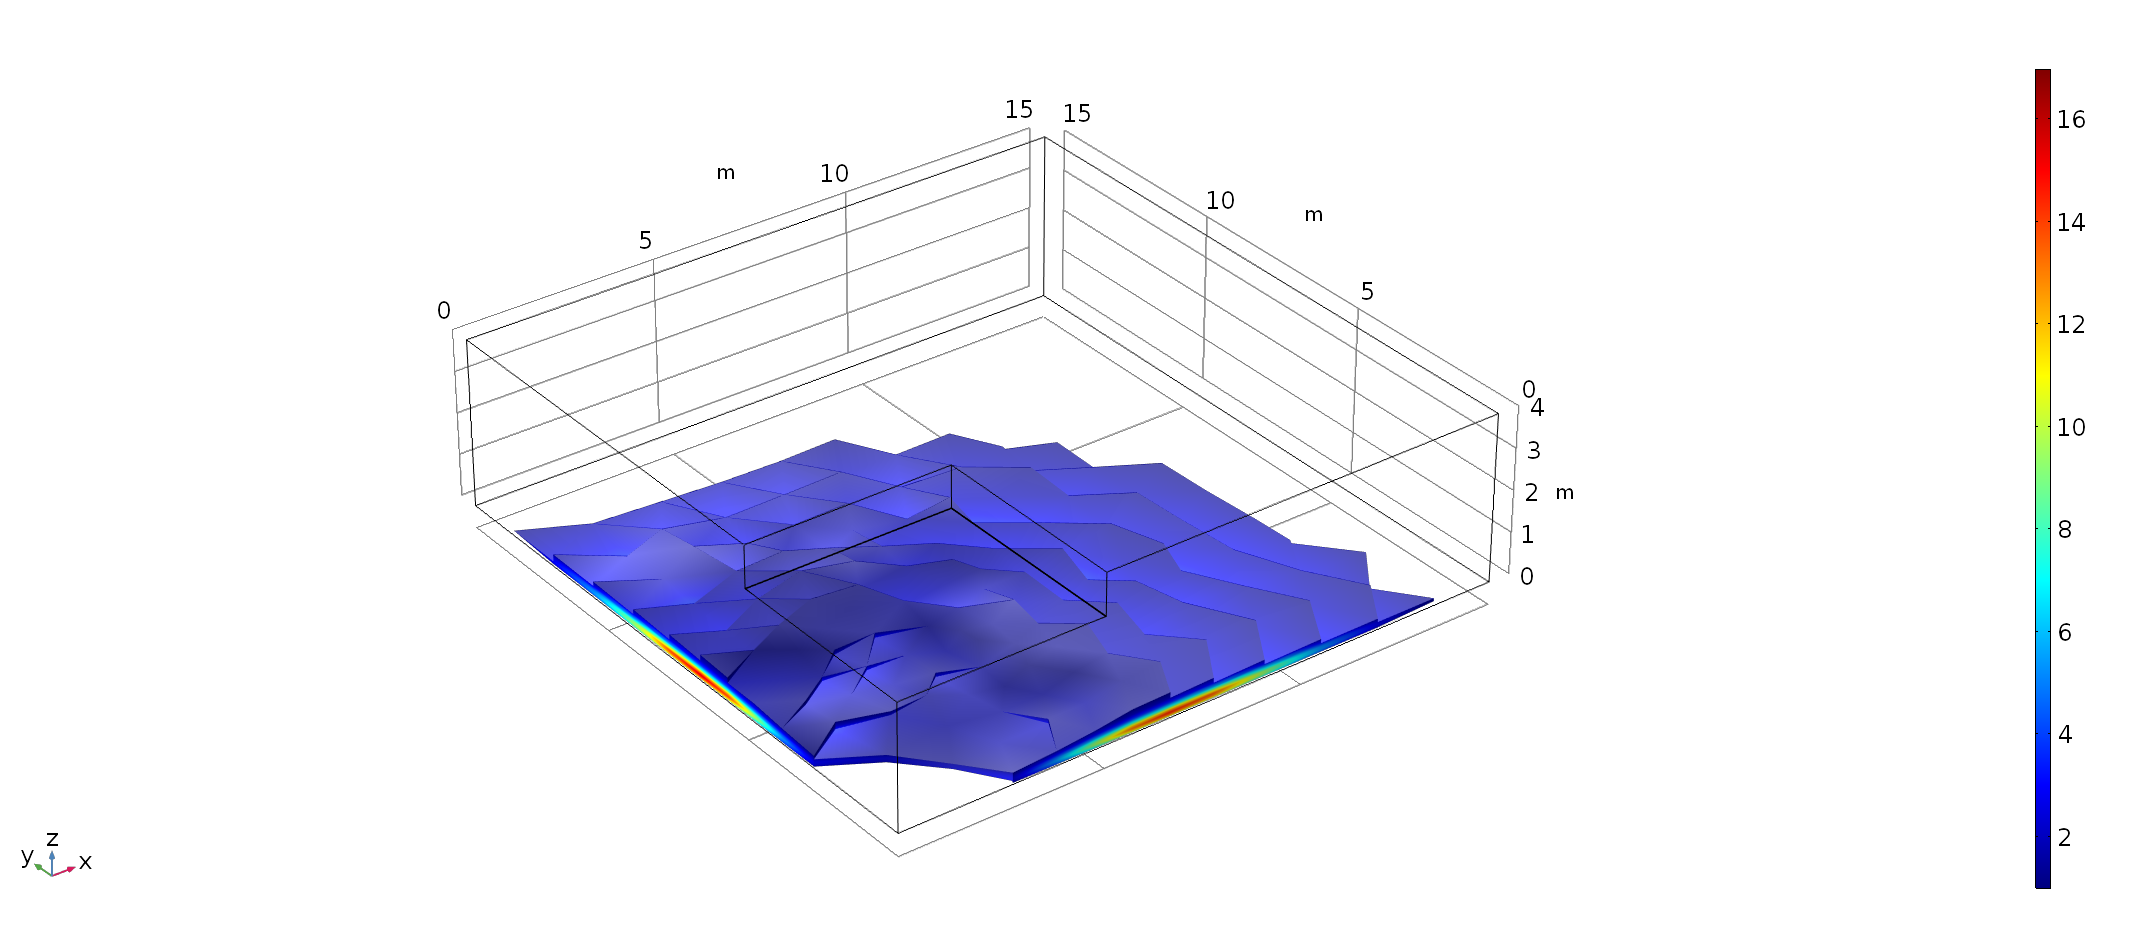
\includegraphics[width=0.75\textwidth]{model_cell_peclet.png}
  \caption{Volume plot showing where the cell Péclet number exceeds 1 and its actual value. I.e. it suggests where the mesh may be improved.}
  \label{fig:model_cell_peclet}
\end{figure}

%\section{Review of Vapor Intrusion Models}\label{sec:model_review}

Mathematical models of VI were from an early stage adopted by investigators and regulators alike.
The primary purpose of these was to providence screening-level risk assessment, i.e. determine if a particular site likely to impacted by VI based upon specific site characteristics such as groundwater contaminant concentration measurements.
This was necessary as VI sites are potentially numerous and a means to prioritize was needed.
Since such models had successfully been used in radon intrusion, similar ones were, and still are, developed for VI\cite{u.s._environmental_protection_agency_oswer_2015}.\par

The EPA has recommended the use of VI models as a screening risk assessment tool as well as a line-of-evidence in VI investigations in conjunction with field measurements\cite{u.s._environmental_protection_agency_oswer_2015}.
Likewise, various VI models have been used in many European countries in similar applications\cite{provoost_accuracy_2009}.
However, the main obstacle of using models in VI investigations has been, and still is, the difficulties of validating them.
These difficulties stem from the lack of available comprehensive datasets of VI sites and the inability to change the CSM that underpins the development of many of the most widely used VI models, e.g. if a particular model assumes the only contaminant source is the groundwater, it will never perform well for a site that is characterized by a preferential pathway.
Regardless, VI models offer a means to examine the underlying physics that drive VI and is therefore a valuable research tool.\par

\subsection{Analytical Models}

One of the first, and arguably one of the most well-used VI model was developed by \citeauthor{johnson_heuristic_1991}\cite{johnson_heuristic_1991}, the J\&E model, and was based on much of the modeling work by \citeauthor{nazaroff_predicting_1988}\cite{nazaroff_predicting_1988}.
Here a VI scenario similar to the one presented here was used as a basis for their mode, i.e. a house overlying an infinitely contaminated groundwater source, where contaminant vapors enter through a foundation crack along the perimeter of the foundation.
However, due they sought to develop an analytical model, and therefore certain physics was discarded to enable them to solve the associated PDE.\par

One such is that contaminant transport from the groundwater source to the building foundation was assumed to occur solely through diffusion.
This is a reasonable assumption, as we have seen airflow is very slow in the soil, and especially in the deeper parts of the soil, so in most scenarios, contaminant transport here will be dominated by diffusion.
The contaminant diffusivity was likewise modified using Millington-Quirks model.
However, in their implementation lacked a way to model the soil moisture content, which instead had to be supplied by the user.
Multiple soil layers were supported and with sufficient knowledge or assumptions, and using these, effective diffusivities could be reasonably approximated.\par

While diffusion was assumed to be the only transport mechanism in the soil, both advection and diffusion was assumed to contribute to contaminant entry into the building.
The advective contaminant flow through the foundation crack was here determined using a modified version of Darcy's Law that had been developed previously by Nazaroff\cite{nazaroff_radon_1985} where the driving force was the pressure differential between the indoor and outdoor environments.
However, this approach lacks the relative permeability term from van Genuchten, and requires user input to determine the effective soil permeability.
Contaminant entry through the crack was modeled as transport between two parallel plates, and involved solving the one-dimensional advection-diffusion equation at steady-state.
Indoor contaminant concentration was determined in a similar fashion as presented here, i.e. as a steady-state mass balance between the contaminant entry and expulsion, the latter which is controlled by air exchange rate.\par

In 1998 the EPA implemented the J\&E model as a spreadsheet tool for screening risk, where the user could give a wide variety of input such as air exchange rate, building pressurization, groundwater contaminant concentration, define multiple soil layers with their associated permeabilities and porosities, etc.
Thus, the model was adopted by investigators and regulators as a risk assessment screening tool\cite{u.s._environmental_protection_agency_oswer_2015}.
However, recently many state regulatory agencies have begun to question the use of these sorts of models in VI investigations and currently are given relatively low weight when considering if a site is impacted by VI.\par

Following the J\&E model, a wide variety of analytical models were developed.
These were often similar to the J\&E model in many regards, and often used the same governing equations, but with modifications to accommodate different VI scenarios.
For instance some would have contaminant entry via a crawl space instead of a foundation crack\cite{r._human_1994}, or include soil biodegradation\cite{anderssen_modelling_1997,hers_evaluation_2000}.
\citeauthor{yao_review_2013}\cite{yao_review_2013} wrote a comprehensive review of VI models, discussing their advantages and disadvantages, and which type of scenarios they modeled.
However, due to the analytical nature of these models, some physics was necessary to be omitted in order to develop an analytical solution to that particular problem; this is the inherent disadvantage of analytical VI models.\par

\subsection{Numerical Modeling}

Numerical models do not require the sacrifice of any physical phenomena to be solvable and can be solved in up to three-dimensions, while most analytical models are one-dimensional.
Thus numerical models can offer a more detailed and generalized description of a wider range of VI scenarios.
However, solving numerical models to a satisfactory accuracy can be challenging and often require some expertise on behalf of the user, and such can be less accessible compared to  the analytical spreadsheet models.
But from a research perspective they are far more interesting for examining the physics driving VI.\par

\citeauthor{abreu_effect_2005}\cite{abreu_effect_2005} developed one of the first numerical model of VI - the "ASU model".
This model considered the same VI scenario as in the J\&E model and what has been presented here; an infinitely contaminated groundwater source with contaminant entry into the overlying building occurring through a perimeter foundation crack.


\appendix
\clearpage
\begin{appendices}

  \section{Geometry Generation}

  To create our quarter geometry, only a few simple geometric objects and Boolean operations are required: two cuboids, two rectangles, one Boolean difference operation, and one Boolean join operation.
  Figure \ref{fig:geometry} shows the resulting geometry.
  Note that $z = \SI{0}{\metre}$ is the groundwater/soil interface and the plane of symmetry is around the $(x, y) = (\SI{0}{\metre},\SI{0}{\metre})$ axis\par

  To create the soil surrounding the building using the COMSOL geometry generator:
  \begin{enumerate}
    \item Create a \SI{15}{\metre} by \SI{15}{\metre} by \SI{4}{\metre} block with its base at $(x, y, z) = (\SI{0}{\metre},\SI{0}{\metre},\SI{0}{\metre})$. This is the entire soil domain.
    \item Create a \SI{5}{\metre} by \SI{5}{\metre} by \SI{1}{\metre} block with its base at $(x, y, z) = (\SI{0}{\metre},\SI{0}{\metre},\SI{3}{\metre})$. This will represent the volume that the house take up in the soil, i.e. the underground portion of the basement.
    \item Perform a difference operation, removing the "basement" block from the "soil" block.
  \end{enumerate}
  At this point you will see that a quarter soil domain has been created, with an empty space that represents a house with a foundation slab located \SI{1}{\metre} bgs.\par

  The foundation crack will be modeled by joining two  \SI{1}{\centi\metre} wide strip that spans the perimeter of the surface that represents the house foundation.
  This strip is created by joining two rectangles on foundation surface:
  \begin{enumerate}
    \item Define a work plane \SI{3}{\metre} above zero. This allows us to place two-dimensional objects on the surface of or inside a three-dimensional object.
    \item On the work plane create a \SI{5}{\metre} by \SI{1}{\centi\metre} rectangle with its base at $(x, y) = (\SI{0}{\metre},\SI{5}{\metre} - \SI{1}{\centi\metre})$. This represents one side of the perimeter crack.
    \item Copy the rectangle and rotate it \SI{90}{\degree} around the corner of the foundation, i.e. $(x, y) = (\SI{5}{\metre} - \SI{0.5}{\centi\metre},\SI{5}{\metre} - \SI{0.5}{\centi\metre})$.
    \item Join the two rectangles to create a unified perimeter foundation crack.
  \end{enumerate}
  Now the geometry of this VI scenario is complete.\par

  \section{Properties}
  % TODO: Make sure gravel density data is correct
  % TODO: Flip the table?
  \begin{table}
    \centering
    \caption{Properties and van Genuchten parameters of select soil types\cite{abreu_conceptual_2012}.}
    \label{tbl:soils}
  \begin{tabular}{c c c c c c c}
    \toprule
    \multirow{2}{*}{Soil type} & Permeability & Density & Porosity & Residual moisture & \multicolumn{2}{c}{van Genuchten parameters} \\
    & $\kappa \; \mathrm{(m^2)}$ & $\rho \; \mathrm{(kg/m^3)}$ & $\theta_t$ & $\theta_r$ & $\alpha$ & $m$ \\
    \hline
    Sand & \num{9.9e-12} & 1430 & 0.38 & \num{5.3e-2} & 3.5 & 3.2 \\
    Loamy sand  & \num{1.6e-12} & 1430 & 0.39 & \num{4.9e-2} & 3.5 & 1.7 \\
    Sandy loam  & \num{5.9e-13}  & 1460 & 0.39 & \num{3.9e-2} & 2.7 & 1.4 \\
    Sandy clay loam  & \num{2.0e-13} & 1430 & 0.38 & \num{6.3e-2} & 2.1 & 1.3 \\
    Loam  & \num{1.9e-13}& 1380 & 0.40 & \num{6.1e-2} & 1.5 & 1.5 \\
    Silt loam  & \num{2.8e-13} & 1380 & 0.44 & \num{6.5e-2} & 0.51 & 1.7 \\
    Clay loam  & \num{1.3e-13}  & 1500 & 0.44 & \num{7.9e-2} & 1.6 & 1.4 \\
    Silty clay loam & \num{1.7e-13} & 1390 & 0.48 & \num{9.0e-2} & 0.84 & 1.5 \\
    Silty clay  & \num{1.5e-13} & 1300 & 0.48 & \num{1.1e-1} & 1.6 & 1.3 \\
    Silt  & \num{6.7e-13} & 1260 & 0.49 & \num{5.0e-2} & 0.66 & 1.7 \\
    Sandy clay  & \num{1.7e-13} & 1470 & 0.39 & \num{1.2e-1} & 3.3 & 1.2 \\
    Clay  & \num{2.3e-13} & 1330 & 0.46 & \num{9.8e-2} & 1.3 & 1.3 \\
    Gravel\cite{dan_capillary_2012} & \num{1.3e-9} & 1430 & 0.42 & \num{5.0e-3} & 100 & 2.19 \\
    \bottomrule
  \end{tabular}
  \end{table}
\end{appendices}

\end{comment}



\begin{comment}
Things to bring up:

- Why is it beneficial to model VI?


- Background on modeling in VI research
-- History & modeling applications
-- Limitations of other people's models
* Should this come before or after my mathematical description of VI?

- Mathematical description of VI modeling
* Start with a non-technical description of a CSM and the processes/physics underlying it. A nice graph showing all of it (including labeled physics and fluxes) would be nice.

- Short description of FEM
-- COMSOL
-- Basic mathematical concept
-- Advantages/disadvantages of this approach compared to others, i.e. why pick FEM over other numerical schemes?
-- Meshing
\end{comment}


\end{document}
